\documentclass[a4paper]{article}

\usepackage[english]{babel}
\usepackage[utf8]{inputenc}
\usepackage{amsmath}
\usepackage{float}
\usepackage{graphicx}
\usepackage{subcaption}
\usepackage[colorinlistoftodos]{todonotes}
\usepackage{hyperref}
\usepackage{lineno}
\usepackage{setspace}
\usepackage{soul}
\usepackage{multirow}
\usepackage[affil-it]{authblk}
\usepackage{verbatim}
\usepackage[bottom]{footmisc}
\usepackage[left=0.6in,right=0.6in,top=1in,bottom=1in]{geometry}
\usepackage[margin=0.6in]{caption}
\usepackage{multicol}
\usepackage{lineno}
\usepackage{array}
\linenumbers
\linespread{1.1}

\usepackage{listings}
\usepackage{xcolor}
\lstset { %
    language=C++,
    backgroundcolor=\color{black!5}, % set backgroundcolor
    basicstyle=\footnotesize,% basic font setting
}

\title{Measurement of $\nu_e$ interactions at low energy with the MicroBooNE Experiment}

\author[1]{Sophie Berkman}
\author[1]{David Caratelli}
\author[2]{Ivan Caro Terrazas}
\author[1]{Giuseppe Cerati}
\author[3]{Nicolo Foppiani}
\author[1]{Elena Gramellini}
\author[3]{Roxanne Guenette}
\author[2]{Ryan LaZur}
\author[2]{Michael Mooney}
\author[3]{Sebasten Prince}
\author[3,4]{Roberto Soleti}
\author[3,4]{Wouter Van De Ponteele}
\author[1]{Maya Wospakrik}
\affil[1]{Fermi National Accelerator Laboratory}
\affil[2]{Colorado State University}
\affil[3]{Harvard University}
\affil[4]{University of Oxford}
%\date{\today}	


\begin{document}

\maketitle

\abstract{The analysis presented in this note uses data from the MicroBooNE Experiment to measure  $\nu_e$ interactions from the Booster Neutrino Beamline using the Pandora reconstruction framework. Our goal is addressing the nature of the anomalous excess of low-energy events with EM activity in the final state as recorded by the MiniBooNE experiment. In this document, we outline the analysis strategy, focusing on the reconstruction and event selections performed, the evaluation of systematics associated to detector, flux, and neutrino-interaction modeling, and the expected sensitivity to the MB-$\nu_e$ LEE model utilizing the available BNB dataset of 10.1$\times 10^{20}$ POT. }

\tableofcontents

\newpage

%\begin{multicols}{1}
\section{Introduction to the $\nu_e$ analysis}
In this section, we provide the big picture view of the complete Pandora $\nu_e$ analysis, starting from our selection philosophy and ending with our strategy regarding systematics. A deeper dive into on each topic is provided in note's following sections. 

\begin{comment}
\par The analysis presented in this note consists in a measurement of $\nu_e$ interactions from the BNB with MicroBooNE in the low-energy ($\lt 800$ MeV) regime aimed at addressing the electron or photon-like nature of MiniBooNE's recorded excess of events with EM activity in the final state. 
This analysis focuses on being able to measure low-energy $\nu_e$ interactions. The reason for this is to have sensitivity to a potential signature of anomalous $\nu_e$ events which comprise MiniBooNE's Low Energy Excess (LEE). This excess was recorded below 800 MeV in reconstructed visible energy (most hadronic activity, especially protons, because below Cherenkov threshold). 
\end{comment}

\subsection{$\nu_e$ Selection Philosophy \textcolor{green}{David ... (P.R. Elena) }}
\par Several proposals have been made to explain the nature of the MiniBooNE LEE anomaly. It is fair to say that a large amount of uncertainty remains in the community regarding what may have generated such an excess of EM events: this analysis works within the $\nu_e$ excess hypothesis.  To best explore the potential new physics in the $\nu_e$ channel at low energy, this analysis aims to perform an inclusive multi-channel measurement of $\nu_e$ interactions without relying on kinematic variables which depend upon neutrino-interaction models.   \textcolor{red}{A multi-channel approach potentially reduces the systematics dependent on the chosen interaction model as well as builds a stronger confidence against  issues in the MC simulation. Please check if this is a pile of BS}.

\par By performing three different $\nu_e$ selections, we aim at isolating three channel topologies: the $\nu_e$ inclusive, 1$e$N$p$0$\pi$, and a 1$e$0$p$0$\pi$ channels. A schematic summarizing the strengths and features of each selection is shown in table~\ref{tab:selectionsNue}. The 1$e$N$p$0$\pi$ and 1$e$0$p$0$\pi$ selections are orthogonal and share a common pre-selection, which splits at the stage in which presence of a final state proton in the event is determined; these two channels combined match the MiniBooNE signal channel (1$e$X$p$0$\pi$). The inclusive $\nu_e$ selection currently is developed independently of the other two selections: therefore, its selected events are not orthogonal to the 1$e$X$p$0$\pi$ pool of candidates.
%\textcolor{red}{Should we add that our main selection is the 1$e$N$p$0$\pi$? }

\begin{comment}
\par We perform three $\nu_e$ selections, each aimed at leveraging particular strengths, and designed with cuts tailored to exploit as much information in a given channel topology as possible. The analysis is comprised of a $\nu_e$ inclusive, a 1$e$N$p$0$\pi$, and a 1$e$0$p$0$\pi$ selection. A schematic summarizing the strengths and features of each selection is shown in table~\ref{tab:selectionsNue}. The 1$e$N$p$0$\pi$ and 1$e$0$p$0$\pi$ selections are orthogonal and share a common pre-selection, which splits at the stage in which presence of a final state proton in the event is determined; these two channels combined match the MiniBooNE signal channel (1$e$X$p$0$\pi$). The inclusive $\nu_e$ selection currently is developed independently of the 1$e$N$p$ selection and therefore its selected events are not independent.
\end{comment}



%\begin{figure}[ht]
%\begin{center}
%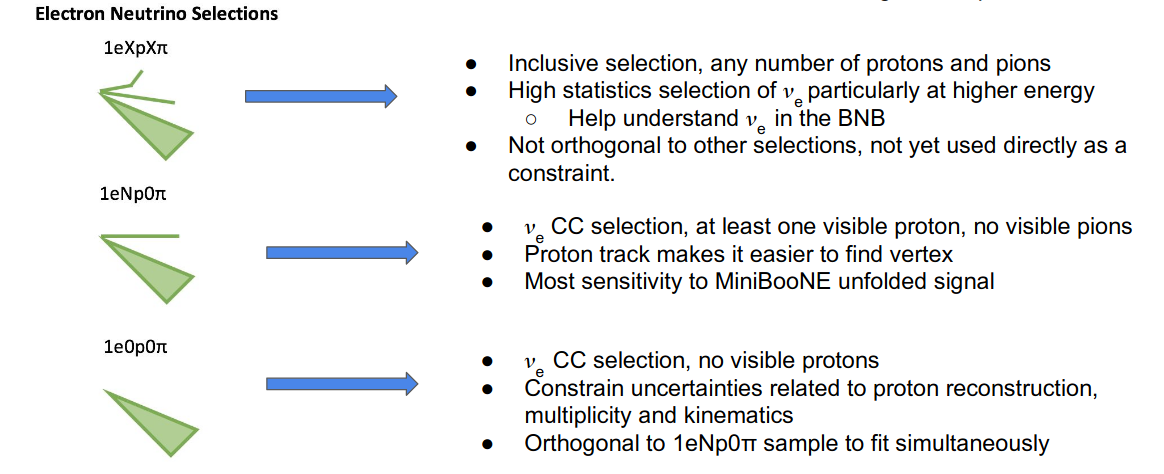
\includegraphics[width=0.85\textwidth]{introduction/nueselections.png}
%\caption{\label{fig:nueselections}Schematic of the three $\nu_e$ selection in this analysis, outlining the goals and strengths of each. In this work, the threshold for a visible proton at truth-level proton is 40 MeV of KE. $N$ refers to one or more and $X$ to any number of final state particles of a given category.}
%\end{center}
%\end{figure}


\begin{table}[ht]
\caption{\label{tab:selectionsNue} Schematic of the three $\nu_e$ selections, outlining the definition and goals of each. In this work, the threshold for a visible proton at truth-level proton is 40 MeV of KE. N refers to one or more and X to any number of final state particles of a given category.}
\centering
%\begin{tabular}{*{3}{ m{0.1\textwidth} }}
\begin{tabular}{ m{0.1\textwidth} | m{0.2\textwidth}  m{0.45\textwidth}  }
Channel & Description & Goal \\
\hline
 \begin{center}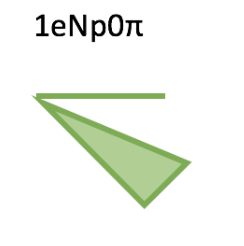
\includegraphics[width=0.1\textwidth]{introduction/1eNp}\end{center}& At least one visible proton and no visible pions & Most sensitive channel to MiniBooNE unfolded signal. The presence of a proton facilitates vertex finding.\\
\hline
 \begin{center}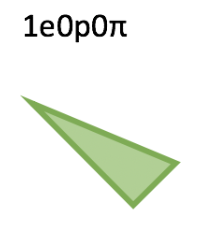
\includegraphics[width=0.1\textwidth]{introduction/1e0p}\end{center}& No visible protons and no visible pions & Constrain uncertainty related to proton reconstruction, multiplicity and kinematics for the 1$e$N$p$0$\pi$ channel.\\
\hline
\begin{center}\includegraphics[width=0.1\textwidth]{introduction/inclusive} \end{center} & Inclusive Selection: any number of protons and pions & Helpful to understand $\nu_e$ in the BNB: high statistic selection, especially at higher energies ($>$ 700 MeV). Not used as a constraint for other channels. \\
\hline
\end{tabular}
\label{tab:gt}
\end{table}


\par %\textbf{agnostic selection} 
In devising the selections presented above, we have deliberately chosen to not rely on cuts that make use of kinematic features of low-energy $\nu_e$ events. This allows the analysis to be agnostic to possible sources of new physics, and limits model dependence associated with assumptions on intrinsic $\nu_e$ interaction kinematics. Furthermore, an agnostic selection strategy allows to explore the kinematics of $\nu_e$ candidate events after their selection, for a full investigation of the origin of a potential anomaly. Implementing this choice requires the ability to fully leverage the information provided by the MicroBooNE LArTPC for $\nu_{\mu}-\nu_e$ and $e-\gamma$ separation. Significant progress has been made in developing tools for this goal, and will be described in subsequent sections. 




\subsection{Signal Model \textcolor{pink}{David}}
\par In order to benchmark the performance of the analysis it is valuable to have a signal model which can be used to assess the analysis' sensitivity.  This section describes the choice of model used for this purpose. It is important to stress that the signal model used serves the purpose of benchmarking the analysis' sensitivity, but the ultimate goal of the analysis remains to measure the rate of $\nu_e$ interactions in the BNB and report whether the observation is consistent or not with MicroBooNE's MC prediction. \textcolor{blue}{Answering whether MicroBooNE's observation is consistent or not with the MiniBooNE LEE anomaly is beyond the scope of this work, and something not achievable without significant work for both MiniBooNE and MicroBooNE.}
\par To test this analysis' sensitivity to MiniBooNE's LEE, a model which can explain it as an excess of $\nu_e$ interactions must be produced, and used to generate simulated events in MicroBooNE. Many such models can be devised, each relying on a given (new) physics production mechanism and set of assumptions on detector response. The primary sensitivity quoted by this analysis will focus on the MiniBooNE-unfolded LEE model, referred to as \textbf{MB-$\nu_e$ LEE} model in this document. In this model, excess LEE events are assumed to be due to $\nu_e$ interactions with a value of true energy obtained by unfolding from the reconstructed CCQE energy of MiniBooNE LEE events, as recorded by MiniBooNE's data. This procedure is perfomed by relying on MiniBooNE's energy smearing matrix. The resulting true neutrino energy distribution is shown in figure~\ref{fig:minibooneunfolded}. There are several limitations to this model worth observing, some technical, others conceptual. On a technical level, the model is composed of a binned event distribution, rather then a parametrized or analytic prediction of the expected $\nu_e$ spectrum. Additionally, no events below 200 MeV of true energy exist in this model. These two factors lead to a granular and truncated model prediction.
\begin{figure}[ht]
\begin{center}
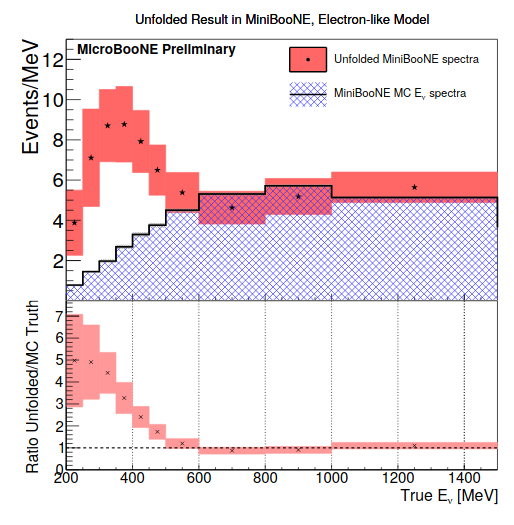
\includegraphics[width=0.45\textwidth]{introduction/unfoldedminiboone.png}
\caption{\label{fig:minibooneunfolded}MB-$\nu_e$ LEE signal model extracted from MiniBooNE's results.}
\end{center}
\end{figure}
Conceptual issues can be raised in association with the various assumptions made to generate the model. These include the strong reliance on MiniBooNE's simulation in order to unfold reconstructed to true neutrino energy, and the choice of such an unfolding procedure (performed as a function of $E_{\rm CCQE}$ rather then EM energy and $\theta$, for example).
\par Ultimately many signal models can be produced to test an analysis' sensitivity, each with its own set of important assumptions and caveats. While reporting sensitivities for the MB-$\nu_e$ LEE model is useful, it is not exhaustive in being able to address MicroBooNE's ability to address MiniBooNE's anomaly. It is especially important to note that this model strongly favors the interpretation of MiniBooNE events as originating from very low energies (200-400 MeV) for which achieving high sensitivity may come at the cost of omitting a robust analysis at higher energies. This is something the analysis tries to avoid by developing an inclusive and kinematically unbiased analysis workflow. At the same time, we explore additional models for sensitivity calculations, most notably a 3+1 sterile-neutrino oscillation model. This is discussed in more detail in section~\ref{sec:sensitivity}.
\par Figure~\ref{fig:nuerate} shows the expected $\nu_e$ rate as a function of true neutrino energy split by final-state topology for the available MicroBooNE dataset of $10.1E20$ POT with a 10 cm FV. MB-$\nu_e$ LEE signal events are shown in orange.
\begin{figure}[H] 
\begin{center}
    \begin{subfigure}[b]{0.45\textwidth}
    \centering
    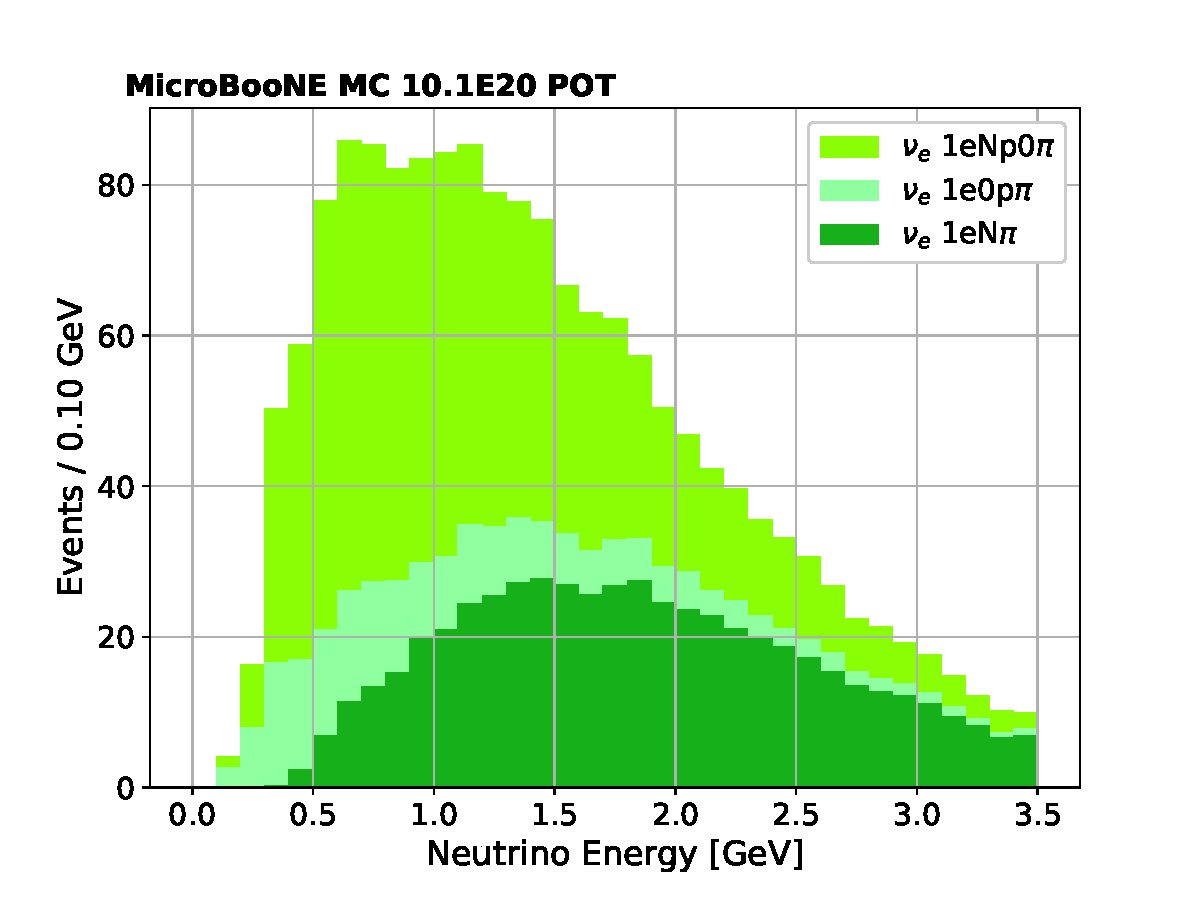
\includegraphics[width=1.00\textwidth]{introduction/nue_rate_MCC9.pdf}
    %\caption{\label{fig:nuerate:prediction}}
    \end{subfigure}
    \begin{subfigure}[b]{0.45\textwidth}
    \centering
    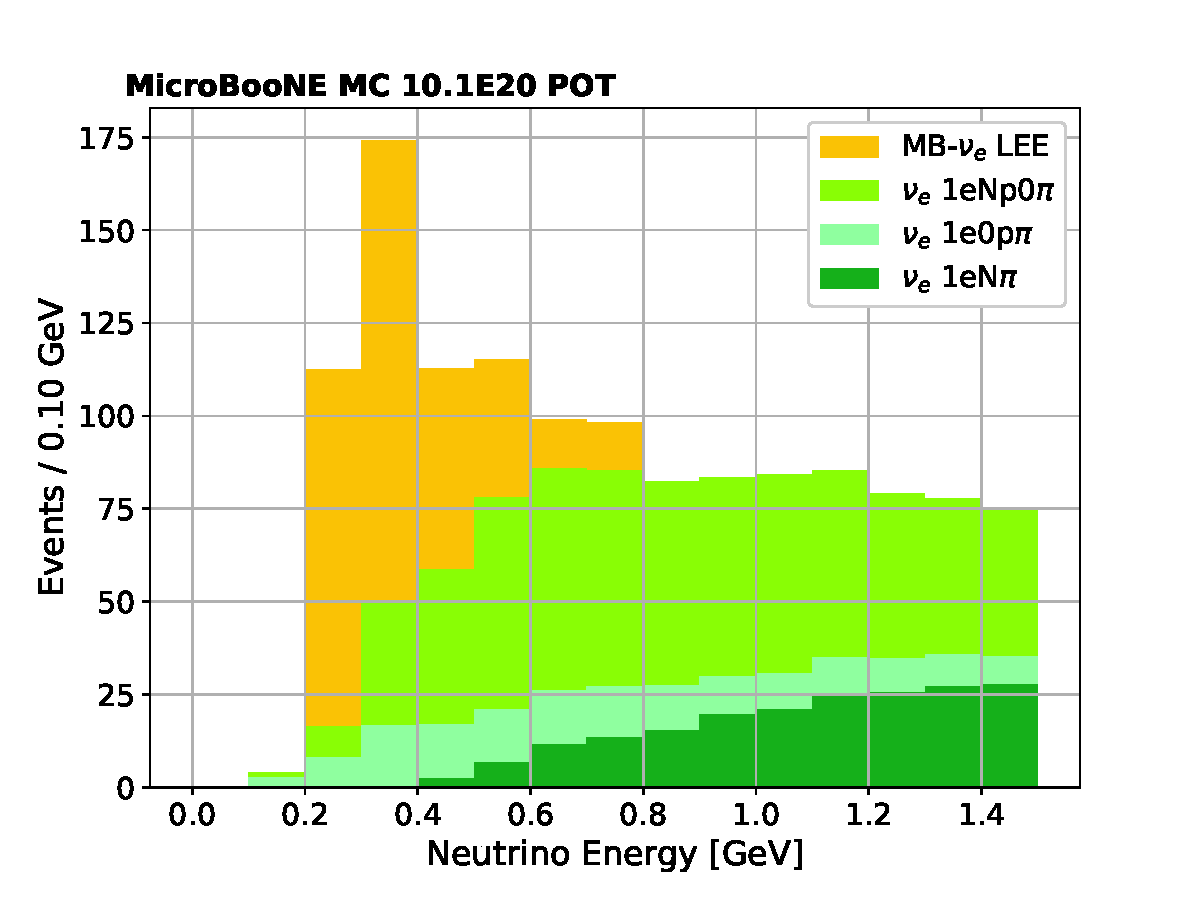
\includegraphics[width=1.00\textwidth]{introduction/nue_rate_MCC9_LEE.pdf}
    %\caption{\label{fig:nuerate:prediction:MC}}
    \end{subfigure}
\caption{\label{fig:nuerate}Expected $\nu_e$ rate in MicroBooNE for $10.1E20$ POT in a 10-cm FV subdivided by event topology (1$e$N$\pi$,1$e$N$p$0$\pi$, and 1$e$N$p$0$\pi$) with, on the right-hand side, the unfolded $MB-\nu_e$ LEE signal prediction}
\end{center}
\end{figure}

\subsection{Goals of the $\nu_{\mu}$ Selection}
\par For the purpose of this analysis, measurements of $\nu_{\mu}$ interactions are aimed at reducing modeling uncertainties for intrinsic $\nu_e$ events and backgrounds, with the goal of reducing systematic uncertainties in order to be able to claim the observation of new physics were a measurement of $\nu_e$ interactions differ significantly from the expected intrinsic rate. This section describes why such a data-driven constraint is needed and what are the choices which motivate the approach taken in this analysis.
\par Event reconstruction and $\nu_e$ identification are only one of the challenges in this analysis. In order to be able to make statements on whether the observed $\nu_e$ rate indicates a presence of new physics, a well understood prediction of the intrinsic $\nu_e$ expectation is needed. Uncertainties in the expected $\nu_e$ rate are associated to reconstruction efficiencies (detector effects) as well as modeling uncertainties in both the $\nu_e$ flux prediction and neutrino-argon cross-section modeling. Here we focus on describing the strategy employed to deal with flux and cross-section uncertainties. Modeling uncertainties in the expected rate of $\nu_e$ interaction are large, and can limit the ability to associate a $\nu_e$ measurement with potential new physics if not constrained through additional measurements. Flux uncertainties for $\nu_e$ are $\mathcal{O}$(10\%) above 800 MeV and grow to 40\% at 200 MeV. Cross-section uncertainties are also large, a consequence of a lack of measurements of $\nu$-Ar cross-sections, particularly at low energy, and the complex modeling of neutrino interactions on a heavy target such as argon. Combining all effects, the uncertainty on the $\nu_e$ interaction rate in the few-hundred MeV energy range in MicroBooNE's could be as high as 100\%.
\par To reduce modeling uncertainties on the expected rate of $\nu_e$ interactions, data-driven constraints are required. These can be performed through measurements of $\nu_{\mu}$ interactions subject to the same uncertainties. In order to constrain flux uncertainties, we rely on the fact that $\nu_e$ and $\nu_{\mu}$ intrinsic to the beam are produced by the decay of the same parent $\pi$ and $K$ flux. Similarly for uncertainties on neutrino interaction modeling, we rely on the common charged-current interaction mode $\nu_{l} + Ar \rightarrow l + X$ for both $\nu_{\mu}$ and $\nu_e$ interactions to constrain interaction uncertainties. 
\par The complexity of $\nu$-Ar interactions and of hadronic interactions in the beamline mean that many different handles and measurements of $\nu_{\mu}$ interactions can play a role in constraining different uncertainties. As examples, measurement of CC and NC $\pi^0$ production constrain resonant interactions and thus $\pi^0$ backgrounds to the $\nu_e$ selection, and measurements of high-energy $\nu_{\mu}$ interactions can help constrain the kaon flux in the beam, which contributes substantially to the production of intrinsic $\nu_e$s. Likewise, measurements of low-energy $\nu_{\mu}$s can help constrain poorly understood $\nu$-Ar interaction models in the few-hundred MeV energy regime, a critical requirement for this analysis. The neutrino identification work developed for this analysis, referred to as \emph{SliceID} and described in section~\ref{sec:sliceID}, is a highly efficient and topology agnostic selection that enables a vast program of $\nu_{\mu}$ measurements, allowing for flexibility in selecting topologies that may have the strongest constraining power and thus most benefit the $\nu_e$ analysis. At the current time, as described in the remainder of this section and in section~\ref{sec:systematics}, the emphasis is on the measurement of low-energy $\nu_{\mu}$ interactions with the goal of constraining the large uncertainties in low-energy $\nu_e$ events which significantly impact the analysis.
\par To further motivate the need for low energy $\nu_{\mu}$ interactions, we describe two important ways in which such a dataset can benefit the reduction of modeling uncertainties for $\nu_e$ interactions. Figure~\ref{fig:numuconstraint:flux} shows the flux correlation for $\nu_{\mu}$ (bottom left) and $\nu_e$ (top right) interactions. Red (blue) areas show large (anti-)correlation. The top-left or bottom-right quadrants show the strength of correlations between the two flavors. For $\nu_e$ energies below 1 GeV, correlations are strongest with $\nu_{\mu}$ interactions at low energy. Figure~\ref{fig:numuconstraint:xsec} shows different cross-section curves for $\nu_{\mu}$ and $\nu_e$ interactions. The dashed and solid curves represent the CCQE cross-section used in MCC8 vs. MCC9 respectively. Below 400 MeV, the difference in event rates for different models is larger then 100\%. The large differences between these curves, particularly at low energy, indicate the strong need to constrain cross-section uncertainties with MicroBooNE's own data. 
\begin{figure}[ht] 
\begin{center}
    \begin{subfigure}[b]{0.42\textwidth}
    \centering
    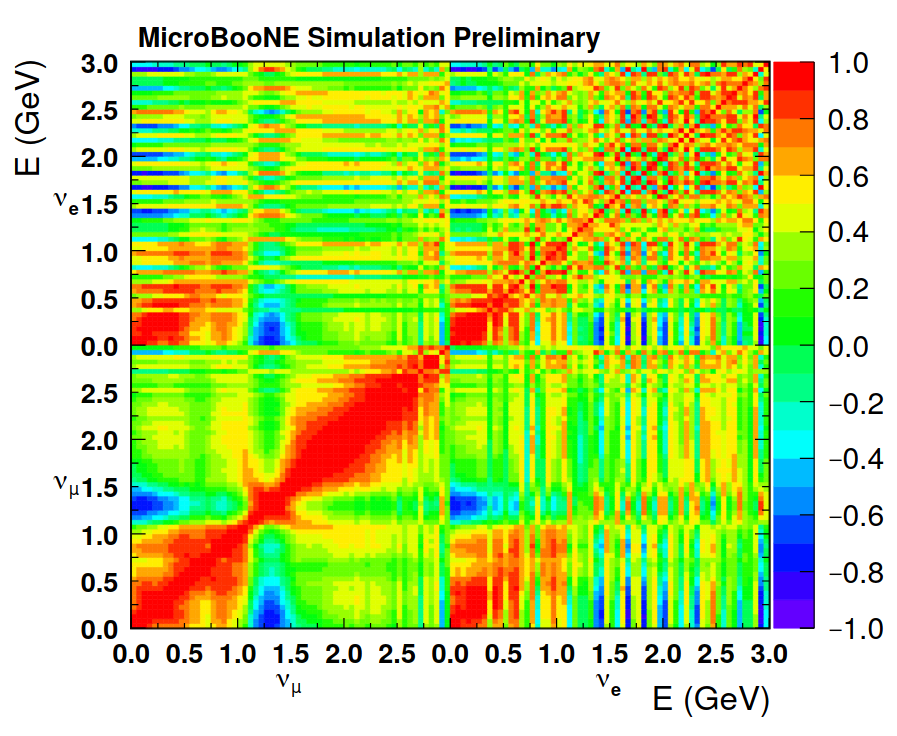
\includegraphics[width=1.00\textwidth]{introduction/fluxcorrelation.png}
    \caption{\label{fig:numuconstraint:flux}$\nu_{\mu}$-$\nu_e$flux correlation matrix}
    \end{subfigure}
    \begin{subfigure}[b]{0.3\textwidth}
    \centering
    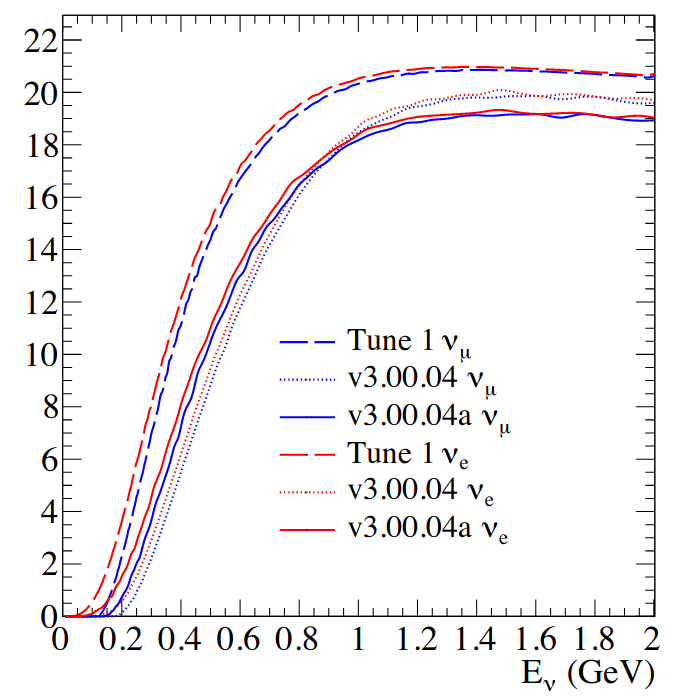
\includegraphics[width=1.00\textwidth]{introduction/xsec_mcc8_mcc9.png}
    \caption{\label{fig:numuconstraint:xsec}different xsec models for CC interactions.}
    \end{subfigure}
\caption{\label{fig:numuconstraint}}
\end{center}
\end{figure}

\subsection{Systematics}
\par This section gives a brief overview of how detector and modeling uncertainties are accounted for in the analysis. The estimation of systematics is performed in section~\ref{sec:systematics}.
\par \noindent \textbf{Detector Systematics}: Detector modeling in MicroBooNE has undergone significant updates in the past year, in part as a result of the large impact that detector systematics have had on 2018 analyses (\textcolor{red}{cite CCpi0,CCincl}). Detector effects with significant impact on the analysis can be broken up into three main categories:
\begin{itemize}
    \item wire-response modeling: the response of MicroBooNE's electronics to drifting charge is a complex subject described in three past publications~\cite{bib:noise,bib:SP1,bib:SP2}. The work of these papers in improving the understanding and modeling of noise and field-response effects has been implemented in the current detector simulation,
    \item Space-Charge modeling: MicroBooNE's space-charge model has changed significantly since 2018, moving from a calculation-based~\cite{bib:SCETN} implementation of electric field distortions to a data-driven E-field map implemented in simulation and reconstruction. Due to the large position distortions (and, though smaller, charge distortions) SCE can significantly impact an analysis through the determination  of fiducial boundaries, tracking and energy resolution.
    \item Scintillation light modeling: MicroBooNE's model of scintillation light production has not changed significantly since the beginning of data-taking, and has known limitations. Of particular importance to this analysis, which aims to use a dataset spanning four years, is the known and significant time-dependent variation of MicroBooNE's light response. This analysis takes several steps to correct for, and mitigate the impact that light mismodeling can have on the analysis. Triggering on low-energy signal $\nu_e$ events, and cosmic-rejection are particularly sensitive to 
\end{itemize}{}
Additional detector effects are ion Recombination...

\subsection{Sensitivity Calculation}


\newpage

\section{Overview of Neutrino Identification: Pandora SliceID}
%\subsection{Event Slicing and Cosmic Removal in Pandora}

The work presented in this note relies on the Pandora approach for event reconstruction~\cite{bib:pandoraub}. The scope of Pandora is to do the low-level pattern-recognition step of the reconstruction, i.e. group hits into clusters, clusters into particles and particles into hierarchies. This section describes how Pandora's pattern-recognition output is combined with scintillation light information to isolate possible candidate neutrino interactions in MicroBooNE events, a process illustrates in the three images of figure~\ref{fig:sliceid}. 

\begin{figure}[ht] 
\begin{center}
    \begin{subfigure}[b]{0.7\textwidth}
    \centering
    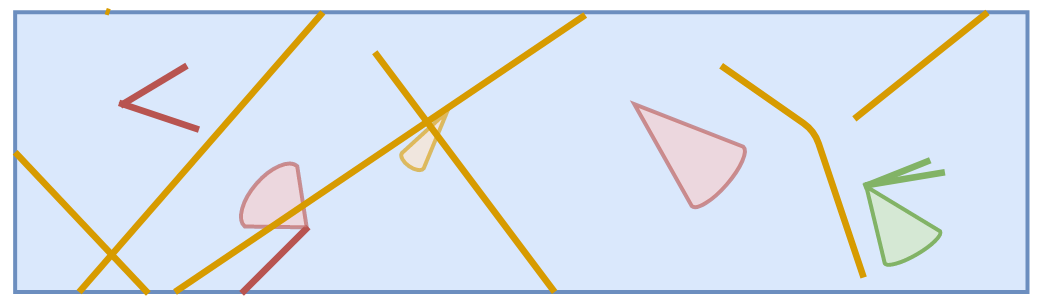
\includegraphics[width=1.00\textwidth]{NuId-Ch2/Images/slice00.png}
    \caption{\label{fig:slcieid:00} Typical event with multiple interactions isolated by Pandora in \emph{slices}.}
    \end{subfigure}
    \begin{subfigure}[b]{0.7\textwidth}
    \centering
    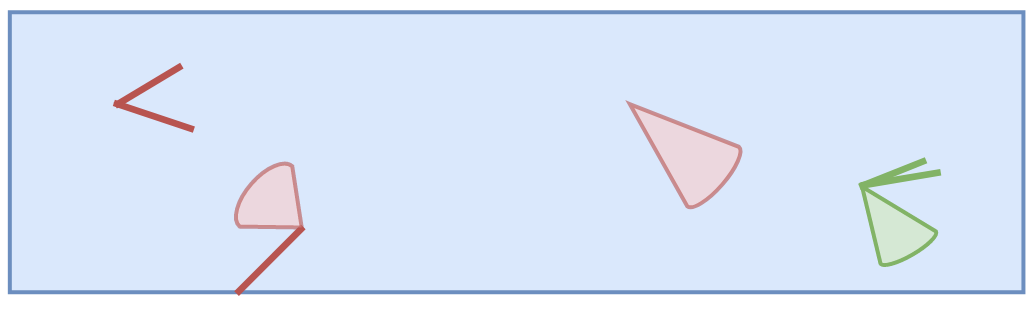
\includegraphics[width=1.00\textwidth]{NuId-Ch2/Images/slice01.png}
    \caption{\label{fig:slcieid:01} Event after the removal of \emph{obvious cosmics} tagged geometrically by Pandora.}
    \end{subfigure}
    \begin{subfigure}[b]{0.7\textwidth}
    \centering
    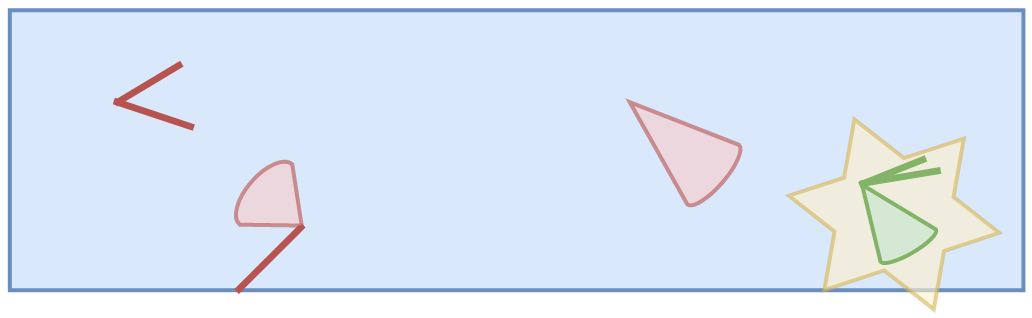
\includegraphics[width=1.00\textwidth]{NuId-Ch2/Images/slice02.png}
    \caption{\label{fig:slcieid:01} Implementation of the \texttt{SiceID} tool to isolate possible candidate $\nu$ interactions.}
    \end{subfigure}
\caption{\label{fig:sliceid} Succession of steps in cosmic removal performed using Pandora's topological pattern recognition combined with scintillation light information through the \texttt{SliceID} tool.}
\end{center}
\end{figure}

\subsection{Slicing \textcolor{green}{Wouter ... P.R. Elena}}
The creation of a ``slice" is the first step of the Pandora processing. A slice \textcolor{blue}{is a collection of distinct reconstructed particles which belong to the same interaction (such as a cosmic muon and its Michel electron, or the muon and proton in a 1$\mu$1$p$ neutrino interaction) \st{is a combination of hits on the three different planes which are topological distinct:  it is assumed that different slices correspond to a distinct group of activity in the TPC}}. To produce slices, the Pandora Cosmic Pattern Recognition is first run over all hits, aiming to construct muon tracks and associated $\delta$-rays and Michel electrons under the cosmic hypothesis (fig.~\ref{fig:sliceid:00}). At this stage, obvious cosmic activity (through-going or out-of-time muons) is tagged using geometric information. The obvious cosmic tagged hits are discarded (fig.~\ref{fig:sliceid:01}); the filtered hit collection is used as input to the Pandora Consolidated Pattern Recognition which reconstruct slices under the neutrino hypothesis. Each slice is now reconstructed both under the cosmic hypothesis and the neutrino hypothesis. A typical event contains approximately 5 slices. 

\subsubsection{Clustering and Vertex Finding \textcolor{green}{Wouter}} 
Pandora computes the 2D clustering on the hits in each slice and in each plane separately. Then, a number of 3D candidate vertices is created by finding positions that project down on to the ends of the available 2D clusters. All of the possible candidates are fed into the support vector machine (SVM) vertex selection, and the most appropriate one is chosen. This 3D vertex is used to split any existing clusters that straddle the vertex. Then, the cluster matching algorithms are run, where the clusters are compared between views and modified to improve the matching.

\subsection{SliceID : Cosmic Removal through topology and scintillation-light \textcolor{green}{Wouter}}
\label{sec:sliceID:SliceID}
\par After the Pandora pattern-recognition algorithm suite has isolated individual interactions into reconstructed \emph{slices} and removed those that are either through-going or out-of-time, the remaining task is to identify which (if any) slice is associated to a neutrino interaction. This is done by relying on scintillation light information to reject slices incompatible with light recorded in-time with the beam. Additionally, topological cuts aimed at rejecting stopping-muon events which enter the TPC are used. The SliceID is at the core of all neutrino selections performed in this analysis, and serves as the first, common step in the analysis, responsible for the majority of cosmic-rejection.
\\
\par We have three handles that we use to distinguish between neutrino and cosmic-ray slices.
\begin{enumerate}
    \item Simple optical pre-selection cuts - is the slice totally inconsistent with the beam flash?
    \item Topological score - to what extent does the slice look like a neutrino interaction in the TPC?
    \item Flash-matching score - to what extent does our flash-hypothesis for this slice match the beam flash?
\end{enumerate}
To select the neutrino slice, or reject the event at this stage, the following procedure is followed:
\begin{itemize}
    \item Insist that there is a beam-triggered flash in the beam window.
    \item Only consider slices that pass the optical pre-selection cuts.
    \item If the slice with the largest topological score in the event remains, then select it as the neutrino.
    \item If not, then choose the remaining slice with the largest flash-matching score.
\end{itemize}
Further details on the \texttt{SliceID} tool are available in DocDB 23854 and 22519. Additional documentation for this tool is in preparation.

The performance of the SliceID for electron neutrino simulated events is given in~\cref{fig:sliceid}.

\begin{figure}[H]
    \centering
    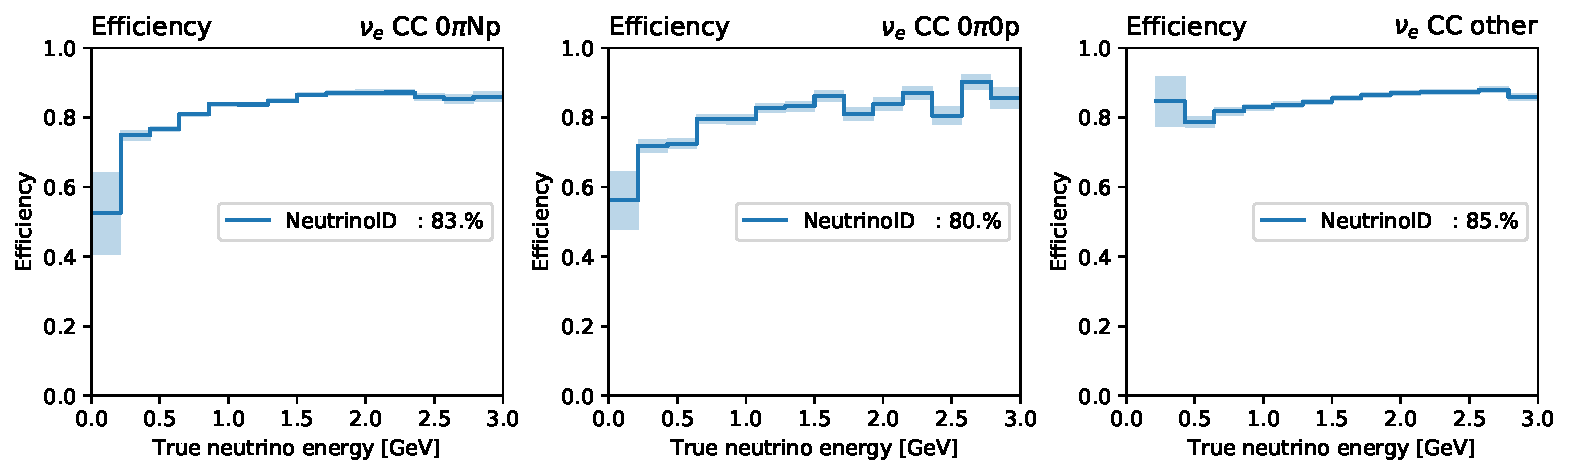
\includegraphics[width=\textwidth]{NuId-Ch2/Images/efficiency_cat_0.pdf}
    \caption{The performance of the SliceID in function of the true neutrino energy for the channel with protons (left), the channel without vertex activity (middle) and events with pions in the final state (right).}
    \label{fig:sliceid}
\end{figure}



\subsection{CRT Veto and Distance Tagger \textcolor{green}{Elena}}
\label{sec:sliceID:CRT}
Contrary to  $\nu_\mu$ interactions and cosmic rays, the charged particles associated to $\nu_e$ interactions are unlikely to deposit energy in the Cosmic Ray Tagger (CRT). Building upon this discriminating factor, the CRT Veto and CRT Distance Tagger are preselection tools which leverage the additional CRT information available for Run 3+ data.
When used, these CRT tools are applied at the pre-selection stage in the following order: CRT Veto, SliceID, CRT Distance Tagger. The CRT tools are especially impactful for the 1e0p channel, where discrimination handles based on the proton PID are obviously missing. \\


\emph{CRT Veto.} %On average, only one in six events passing the MicroBooNE common optical filter is associated to beam-induced activity. The remaining events are triggered by activity that originates outside the TPC: either external beam induced activity or cosmic rays. %Given the $\mathcal{O}(10)$ cosmic ray muons in each drift window, this equates to a starting signal-to-background of $\sim 1 : 60$.
%The CRT Veto looks at CRT activity in time with the beam window. 
The CRT veto looks for a time coincidence between the scintillation light recorded in time with the 1.6 $\mu$s beam-spill (beam-flash) and a CRT hit: if a CRT hit occurs within a 1 $\mu s$ of the beam flash, the event is rejected. For this coincidence, only CRT hits with PE $>$ 100 pe are considered; we do not apply a constraint on the position of the flash nor on the position of the CRT hit. 
The rejection power and efficiency of the CRT veto are calculated using the BNB external and the $\nu_e$ overlay samples, respectively. The BNB external passing rate is $\sim$59\%,  and the $\nu_e$ efficiency greater than $\sim$94\% for all electron neutrino energies, raising at low energies. \\


\emph{CRT Distance Tagger.} 
The CRT Distance Tagger tool builds upon the standard pandora neutrino vertex reconstruction and the CRT tagging of TPC tracks. A TPC track is tagged with a CRT hit association if the track projection onto a CRT panel and a CRT hit are close in space. 
To perform this association, the track projection to the CRT is calculated under the hypothesis that the associated particle crossed the TPC at the time registered by the CRT hit under consideration; more details on the CRT hit to TPC track match are available in \cite{bib:CRTPresel_Technote}.  The CRT Distance Tagger checks the minimum distance between the reconstructed neutrino vertex and each track tagged with a CRT hit. If the minimum distance is less than 14 cm, the event is rejected. An example event tagged by this cut is shown in Figure~\ref{fig:crtdist00}.  For the CRT Distance Tagger, the BNB external passing rate is $\sim$81\%,  and the $\nu_e$ efficiency greater than $\sim$96\% for all electron neutrino energies, raising at low energies. \\
 
\begin{figure}[h!]
\centering
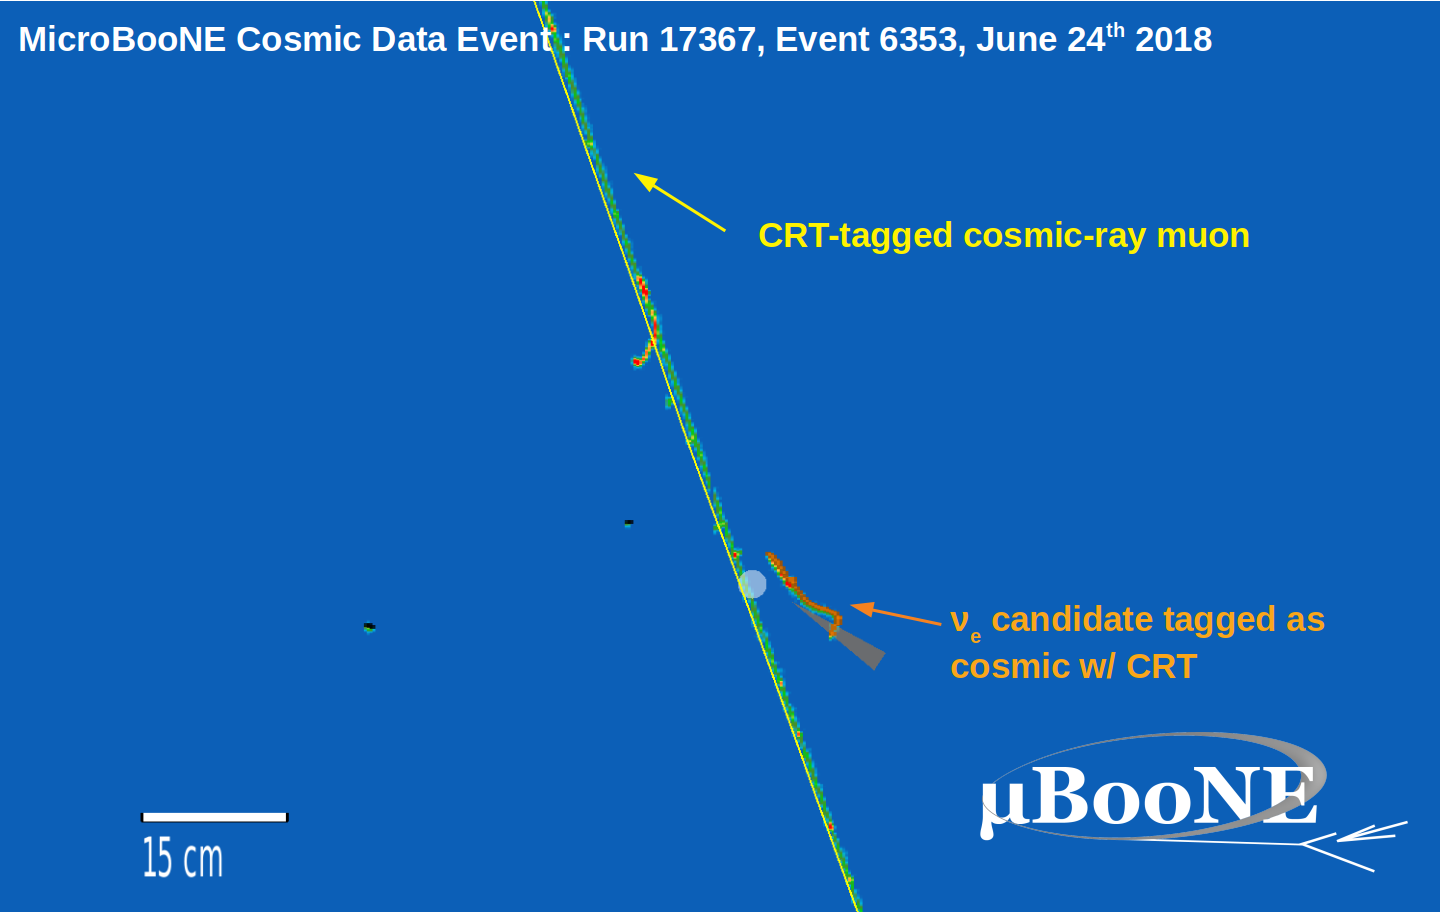
\includegraphics[width=0.4\textwidth]{NuId-Ch2/Images/crttagger_01.png}
\caption{Example $\nu_e$ candidate tagged as cosmic thanks to the CRT distance tagger. From the event one can see that the reconstructed EM shower is associated to EM activity associated to the incoming muon.}
\label{fig:crtdist00}
\end{figure}

An overview of the impact of the CRT on cosmic rejection can be seen in Figure~\ref{fig:crt} where the beam-time distribution for the $8E18$ POT Run 3 open dataset is shown after SliceID (left), and after SliceID and CRT cosmic-tagging tools (both CRT veto and distance tagger) have been applied (right), with EXT backgrounds dropping by more than a factor of 3.
Further details and a preliminary study of the CRT  impact on an electron neutrino preselection can be found in \cite{bib:CRTPresel_Technote}. 

\begin{figure}[ht] 
\begin{center}
    \begin{subfigure}[b]{0.4\textwidth}
    \centering
    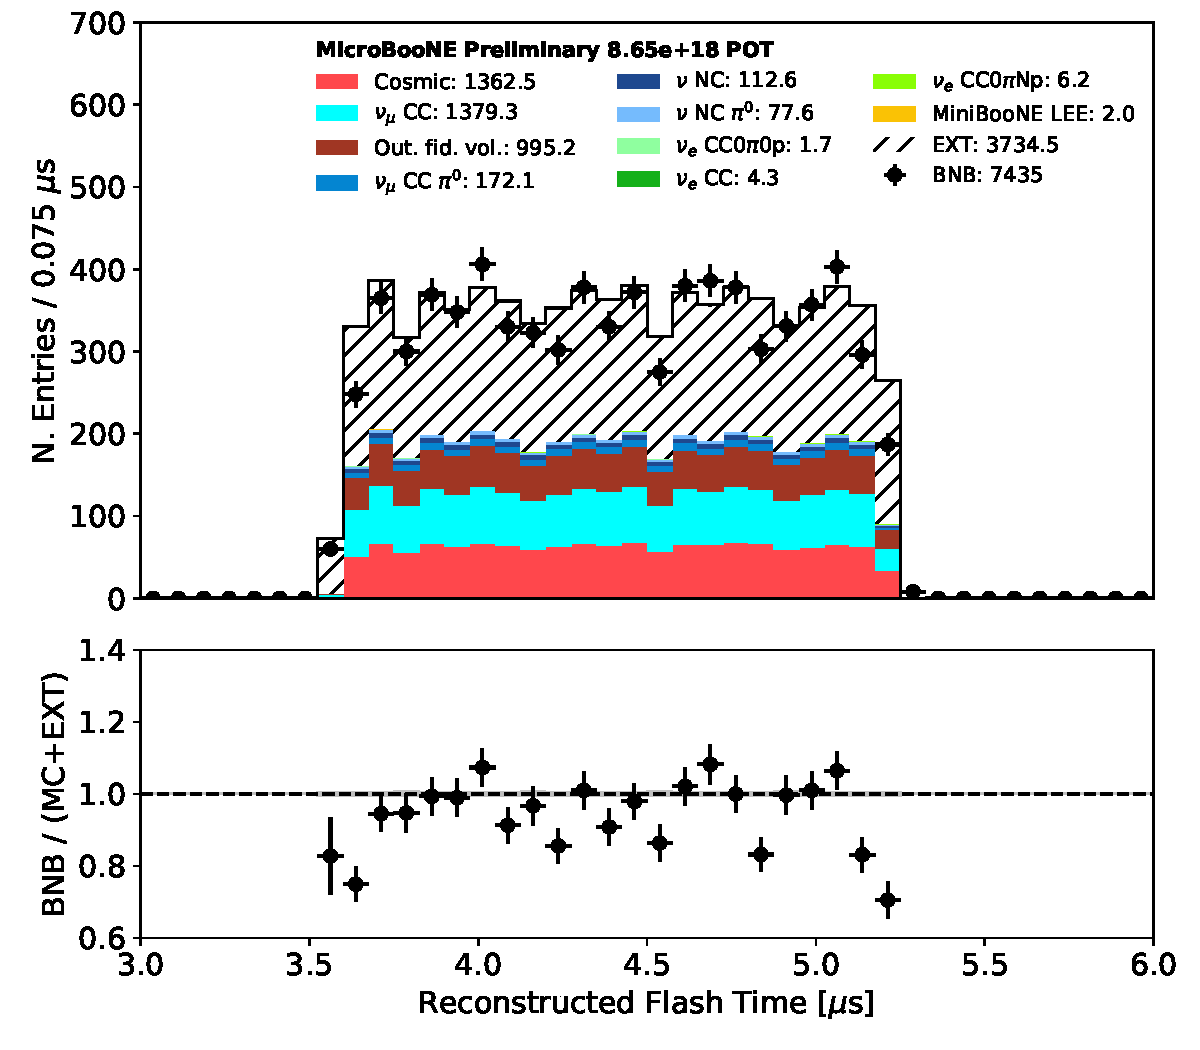
\includegraphics[width=1.00\textwidth]{NuId-Ch2/Images/flash_time_01152020.pdf}
    \caption{\label{fig:crt:pre} no CRT tools.}
    \end{subfigure}
    \begin{subfigure}[b]{0.4\textwidth}
    \centering
    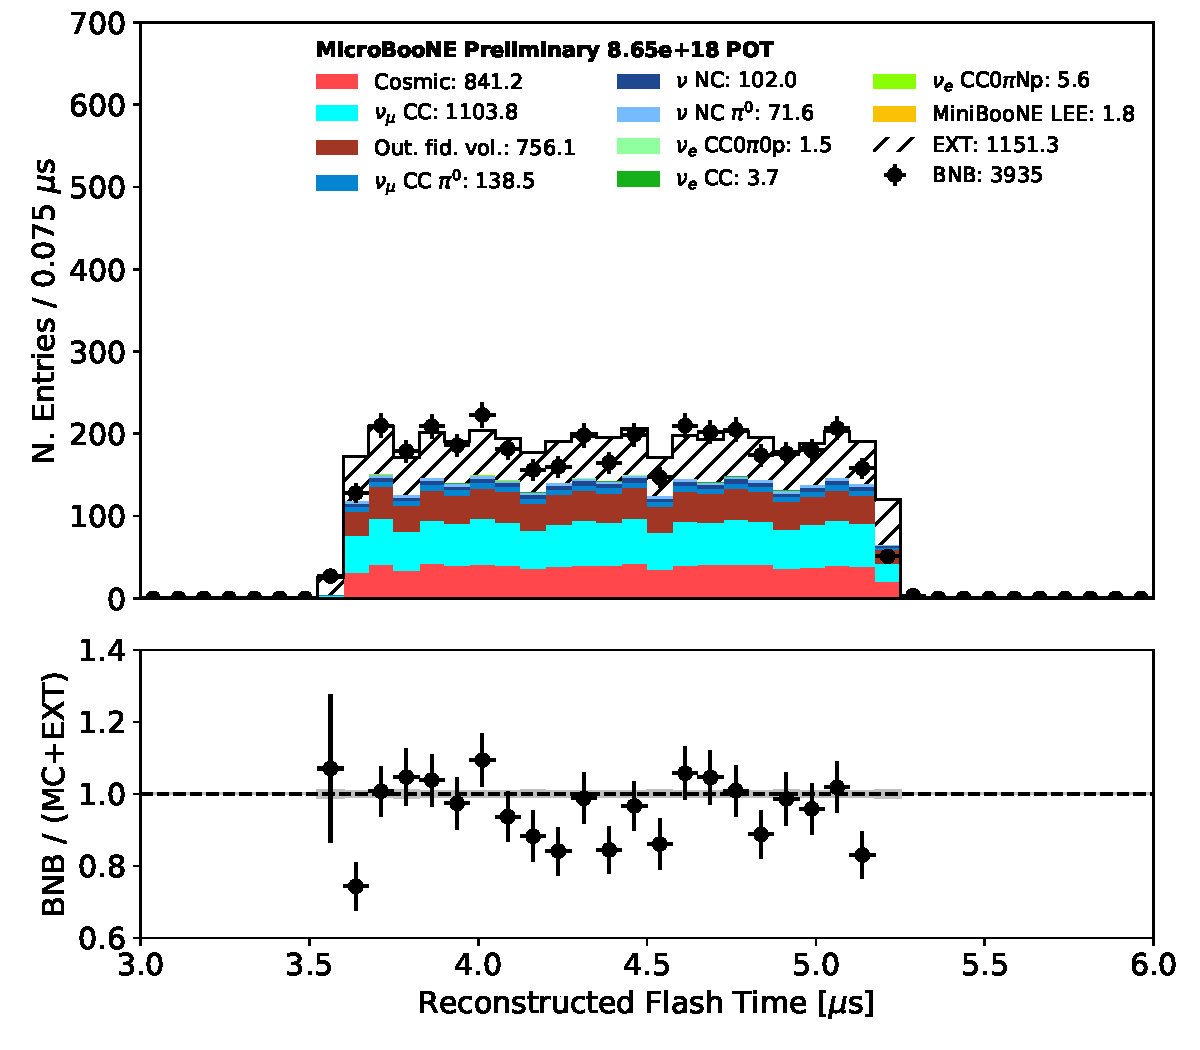
\includegraphics[width=1.00\textwidth]{NuId-Ch2/Images/flash_time_01152020_CRT.pdf}
    \caption{\label{fig:crt:post} with CRT tools.}
    \end{subfigure}
\caption{\label{fig:crt} Beam timing distribution before (left) and after (right) CRT tools have been applied. The EXT contribution is reduced by over a factor of three.}
\end{center}
\end{figure}



\newpage

\section{Neutrino Event Reconstruction \textcolor{red}{Giuseppe, David + ...}}

\subsection{Track and Shower Reconstruction \textcolor{green}{Giuseppe}}
\label{sec:tkshreco}
The output of Pandora~\cite{bib:pandoraub} is organized in a hierarchy of reconstructed Particle Flow Particles (``PFParticles''), which describes the particle content in an observed event as a parent-daughter relationship chain. Final state PFParticles are 3D objects matching clusters of hits in at least two different planes.
Pandora classifies PFParticles as track-like or shower-like base on a Support Vector Machine (SVM) algorithm~\cite{bib:tkshsvm}, producing a score with values between 0 (shower-like) and 1 (track-like).

Pandora processes track-like PFParticles with a sliding linear fit procedure (described in~\cite{bib:pandoraub}) that returns the 3D position and direction at each point along the trajectory (where each point corresponds to a 2D hit). For each point the d$Q$/d$x$ and distance from the track-start are recorded using MicroBooNE's Calorimetry module. This procedure allows to accurately measure d$x$, including small deflections due to the particle's trajectory and SCE offsets, and d$Q$, by incorporating MicroBooNE's full position- and field-dependent relative and absolute charge calibration. From d$Q$/d$x$, d$E$/d$x$ is calculated assuming a fixed recombination correction assuming 2.1 MeV/cm energy loss, but accounting for local variations in the electric field.

We evaluate the energy and 3D direction of shower-like PFParticles with the same algorithm used for the $\pi^0$ reconstruction paper~\cite{bib:pi0reco}. The energy reconstruction accounts for various detector effects, including gain and recombination; corrections for reconstruction effects (hit threshold and imperfect clustering) will be described in Sec.~\ref{sec:ereco}. We also fit showers using a Kalman filter-based procedure~\cite{bib:shrtrackfitter} which aims at identifying the main trunk of the shower by rejecting hits that are longitudinally or transversely displaced from it; the output of this fit is a track object so that the calorimetric tools described above become available for showers as well.

By default, Pandora separates showers and tracks with a cut on the SVM score at 0.5; however, as will be described in later sections, in many cases we choose different cut values, i.e. tighter shower definition for the $\nu_e$ selection and looser for the pi0 control region.

\par The Efficiency of Pandora's reconstruction on $\nu_e$ interactions is evaluated in figure~\ref{fig:nuereco:eff} as a function of true neutrino energy and shows the efficiency for correctly identifying $\nu_e$s in the event in black, and the efficiency for reconstructing $\nu_e$ interactions with a final-state EM shower in blue. The efficiency has a sharp upturn between 100 and 200 MeV, especially in the case when an EM shower is required, and levels off at 80\% and 60\% respectively for the two curves. 
\par At this stage in the analysis, the good efficiency for reconstructing $\nu_e$ events is offset by the very low signal-to-background for $\nu_e$ events in MicroBooNE's data, a consequence of the very small $\nu_e$ content of the beam. With no additional requirement on the reconstructed neutrino, the purity for $\nu_e$ interactions is 0.12\%. After imposing a requirement of one reconstructed shower, the purity grows by almost an order of magnitude, to 1\%. The $\nu$ background composition also changes significantly, with $\pi^0$ backgrounds moving from 14\% to 48\% of all backgrounds.

\begin{figure}[ht] 
\begin{center}
    \begin{subfigure}[b]{0.3\textwidth}
    \centering
    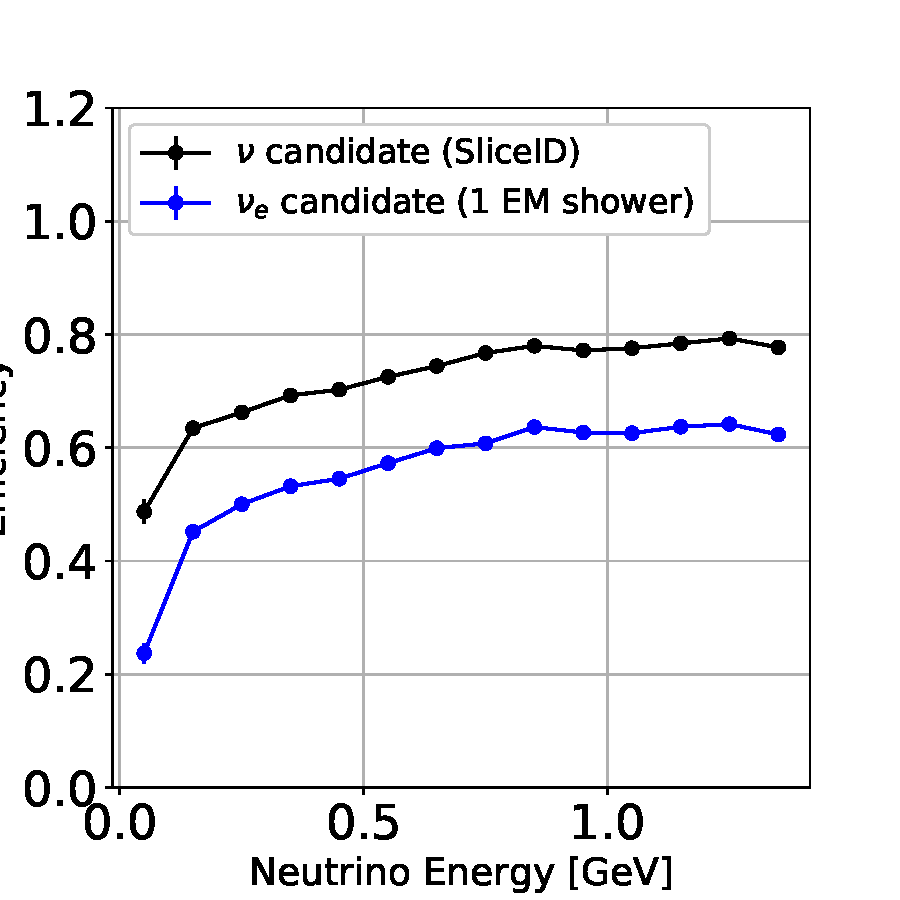
\includegraphics[width=1.00\textwidth]{nureco/nureco_RUN1.pdf}
    \caption{\label{fig:nuereco:eff} $\nu_e$ reco eff.}
    \end{subfigure}
    \begin{subfigure}[b]{0.31\textwidth}
    \centering
    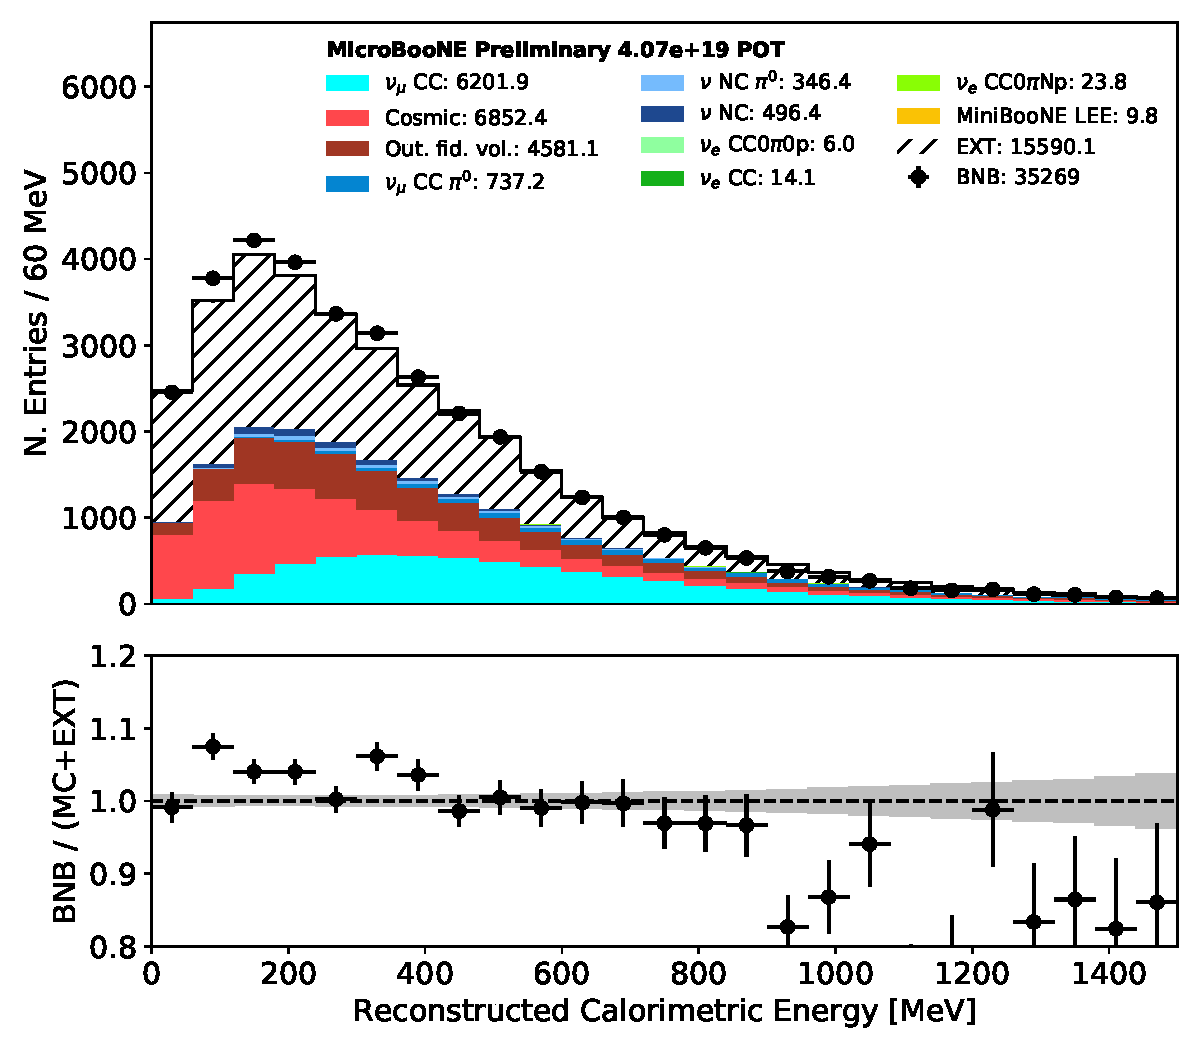
\includegraphics[width=1.00\textwidth]{nureco/NeutrinoEnergy2_01152020.pdf}
    \caption{after SliceID}
    \end{subfigure}
    \begin{subfigure}[b]{0.31\textwidth}
    \centering
    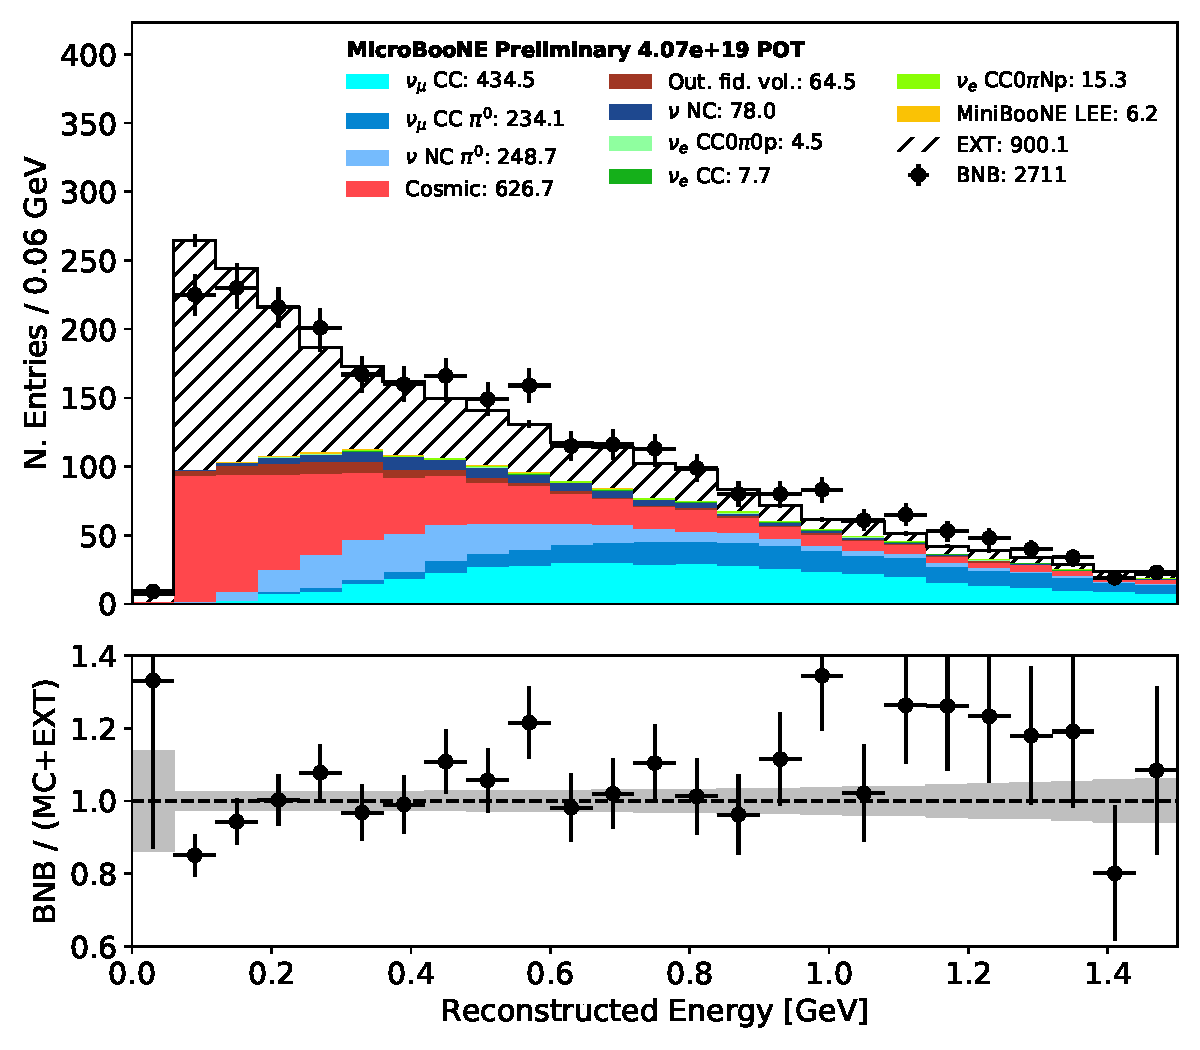
\includegraphics[width=1.00\textwidth]{nureco/reco_e_01152020.pdf}
    \caption{\label{fig:egammasep:dedx} after shower requirement}
    \end{subfigure}
\caption{\label{fig:nuereco}}
\end{center}
\end{figure}

\par The next step in the analysis demands the development of a selection capable of isolating $\nu_e$ interactions rejecting the two order of magnitude larger background rates from $\nu_{\mu}$ neutrinos. This selection will make use of PID and topological information described in the next sections. The strong level of background rejection needed to isolate signal events will inevitably lead to a lower selection efficiency.

\subsection{Particle Identification \textcolor{green}{Nico}}
% GC: this part is now in the previous subsection
%In the neutrino slice, every PFParticle is reconstructed in three different ways:
%\begin{itemize}
%    \item Track, using the standard Pandora Track reconstruction
%    \item Shower, using the standard Pandora Shower reconstruction (is there any modification on top of this?)
%    \item Track-fitted shower, using a dedicated track fitting tool which aims at identifying the main branch of %the shower and fit it as a track. As a result, all the tools developed for the track become available for the %tracks too. For example, for each track-fitted shower, a recob::track and a anab::calorimetry objects are available.
%\end{itemize}
Particle identification is performed with different tools depending the type of candidate a given PFParticle has been selected as.
If the PFParticle has been selected as a muon or proton candidate, so as a track-like object, the identification is performed using the Calorimetry Likelihood tool, which results in the variable Log Likelihood Ratio PID  (section~\ref{subsec:loglikelihoodpid}).
If the PFParticle has been selected as an electron or photon candidate, the identification is performed using several variables described in \ref{subsec:egammaspearation}.

It is noteworthy that this particle identification consists of one or multiple variables, available for the specific PFParticle, that may or may not depend on the rest of the slice. 
For example, the shower dE/dx depends only on the PFParticle itself, whereas the track-shower separation relies also on additional objects identified in the slice.

The value of the cuts applied on these variables depend not only on the general level of efficiency and mis-identification one may want to achieve in distinguishing two kind of particles (electrons from photons, for example), but also on the mixture of backgrounds, which eventually depends on the specific selection the analyser is performing.

\subsubsection{Log Likelihood Ratio Particle ID \textcolor{red}{Nico}}
\label{subsec:loglikelihoodpid}


\subsubsection{$e$/$\gamma$ Separation}
\label{subsec:egammaspearation}
\par Distinguishing electron from photon EM-showers is one of the crucial steps required to perform a measurement of $\nu_e$ interactions in the BNB beam. Photon backgrounds to a $\nu_e$ measurement are largely caused by neutrino interactions with $\pi^0 \rightarrow \gamma\gamma$ in the final state, which dominate the $\nu_e$ event rate by at least an order of magnitude. Three key features distinguish events with $\pi^0$ induced photon showers from $\nu_e$ interactions: (a) the presence of two final state EM showers. (b) the non-zero conversion distance separating the neutrino interaction vertex from the shower start point, and (c) the calorimetric separation via $dE$/$dx$ due to the overlapping ionization segment of $e^+$/$e^-$ pair-conversions through which most $\gamma$ showers manifest themselves. Figure~\ref{fig:egammasep} shows how, at reconstruction level, each of these features can aid in $e$/$\gamma$ separation. This section describes how each of the items above is utilized in the analysis on a technical level, what performance is obtained and challenges (both physics- and reconstruction-driven) are encountered in doing so.

\begin{figure}[ht] 
\begin{center}
    \begin{subfigure}[b]{0.31\textwidth}
    \centering
    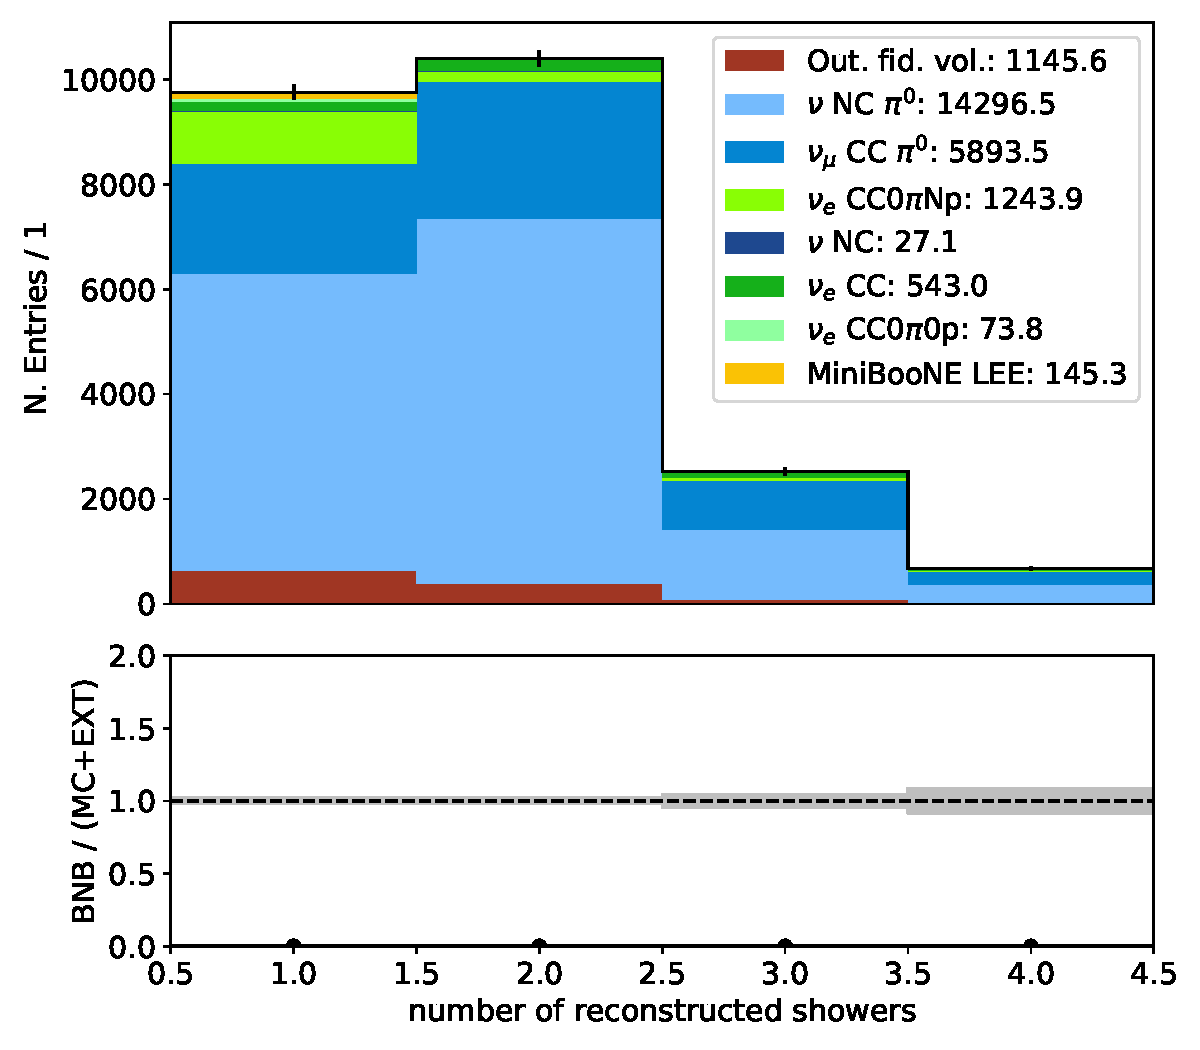
\includegraphics[width=1.00\textwidth]{egamma/n_showers_contained_01022020.pdf}
    \caption{number of reconstructed showers}
    \end{subfigure}
    \begin{subfigure}[b]{0.31\textwidth}
    \centering
    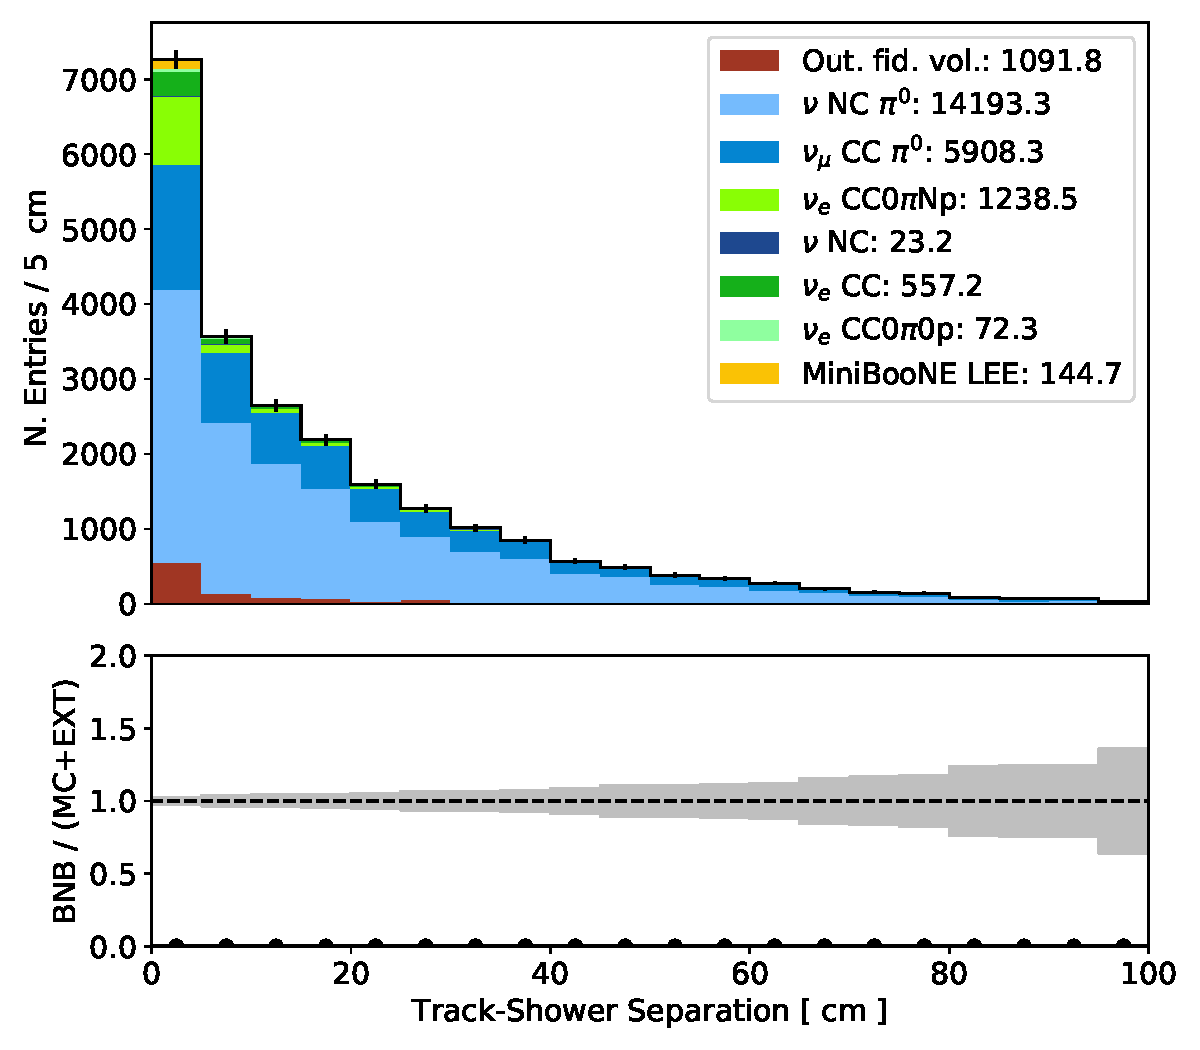
\includegraphics[width=1.00\textwidth]{egamma/tksh_distance_01022020.pdf}
    \caption{track-shower separation}
    \end{subfigure}
    \begin{subfigure}[b]{0.31\textwidth}
    \centering
    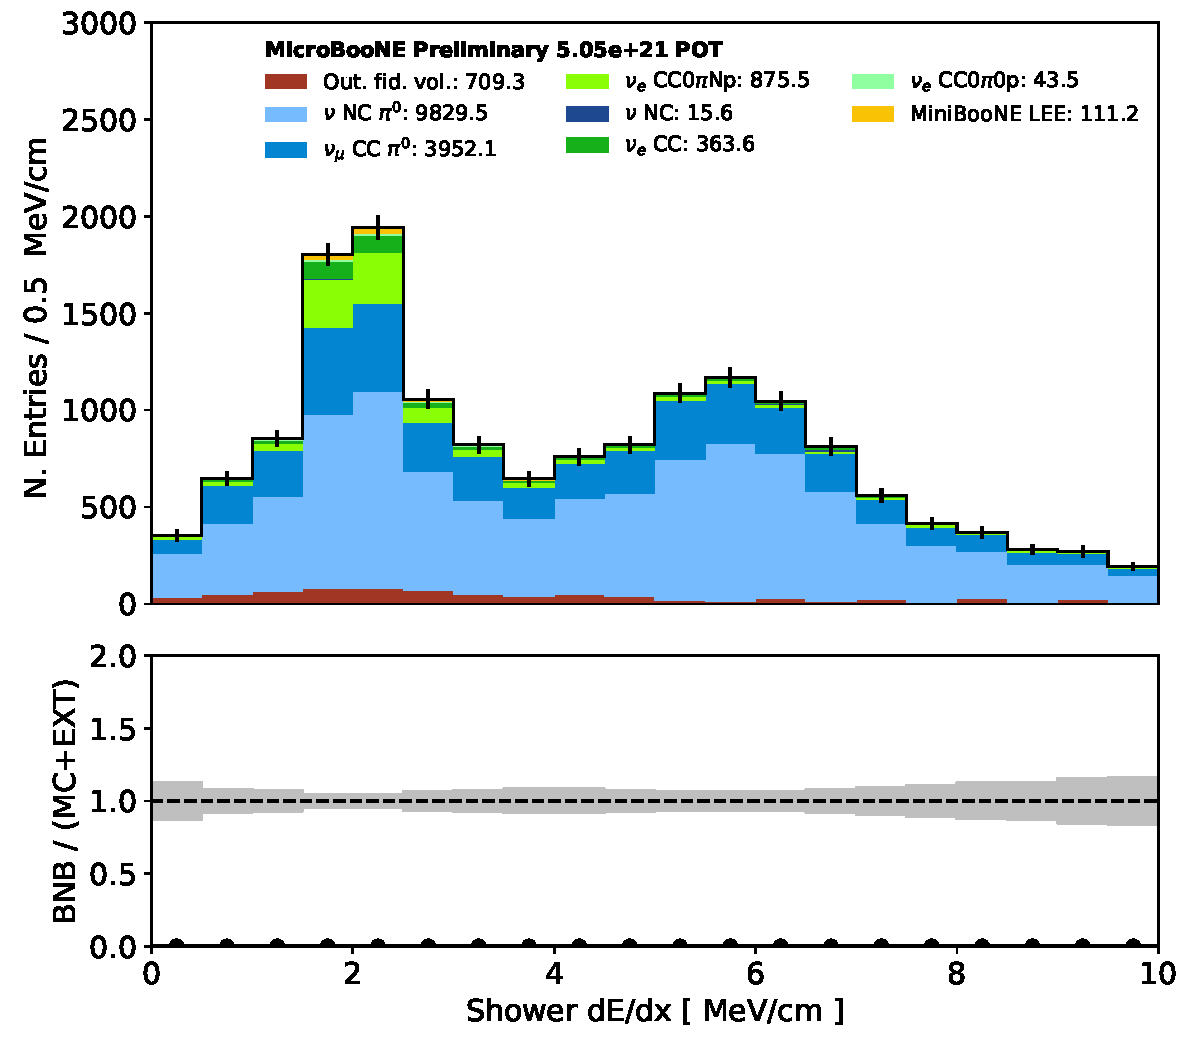
\includegraphics[width=1.00\textwidth]{egamma/shr_tkfit_dedx_Y_01022020.pdf}
    \caption{\label{fig:egammasep:dedx} reconstructed shower $dE$/$dx$}
    \end{subfigure}
\caption{\label{fig:egammasep}Comparison of simulated $\nu_e$ (green) vs. $\nu_{\mu} \rightarrow \pi^0 + X$ (blue) for the three discriminating variables of (a) number of showers, (b) vertex distance, and (c) $dE$/$dx$. Distributions are POT-normalized but do not conatain non-$\nu_e$ or non-$\pi^0$ events, nor on/off-beam data distributions.}
\end{center}
\end{figure}

\par \textbf{two-shower requirement} Requiring a single reconstructed shower keeps 68\% of $\nu_e$ interactions (with no $\pi^0$ in the final state) while removing 61\% of $\nu_{\mu}$ events with at least one $\pi^0$ in the final state. The fraction of kept $\nu_e$s grows to 79\% when looking below 800 MeV of true energy (the focus of this analysis). Rejection of $\nu_e$s is largely due to events where the electron shower is reconstructed as two separate EM showers, often closely aligned in 3D. Events with final state $\pi^0$s are reconstructed with a single EM shower in the final state because either the second photon escapes the TPC active volume completely (irreducible) or because the second shower is not reconstructed. The dominant causes of this second case are (1) highly-boosted $\pi^0$ decays, in which two aligned photons are merged into one shower and (2) photons which go undetected, often low in energy (below 100 MeV). Additional discriminating variables which aim to recover the reconstruction-related mis-ID of (1) and (2) are utilized in the analysis and presented in Sec.~\ref{sec:nueselection:tools}.
\par \textbf{track-shower separation} For events where hadronic activity at the neutrino interaction vertex (i.e. final-state protons) is visible, a clear gap between the vertex and the shower start-point can be used to reject $\gamma$ backgrounds. This is a powerful background mitigation tool in the 1$e$N$p$ $\nu_e$ selection. Two factors determine the performance of such a tool: the ability to detect protons and other hadronic activity at the vertex and the accuracy with which the shower start-point is reconstructed. The shower start-point reconstruction accuracy determines the level of background rejection one can obtain, as $\gamma$ showers lead to an exponential conversion-distance distribution. A 1 vs. 5 cm track-shower separation cuts lead to 95\% vs 74\% mis-ID respectively, but causes a drop in selection efficiency for 1$e$N$p$ events from 72\% to 28\%. In order to enhance the ability to isolate $\nu_e$ events in the 1$e$N$p$ selection through vertex-displacement, different metrics are used to measure the presence of a gap between an electron and proton candidate. These will be described in section~\ref{sec:nueselection:tools}. It is important to note that this background mitigation strategy is not applicable to single-electron searches, which are an important contribution to $\nu_e$ interactions, especially in the low-energy regime.
\par \textbf{shower d$E$/d$x$} The majority of photons manifest themselves in a TPC through the ionization released by the $e^+$/$e^-$ pair produced via pair-conversion. The electron-positron pair is highly aligned and overlaps on the mm-scale, leading to a doubly-ionizing charge-segment compared to electron showers. To measure this, we use the track fit of the main shower trunk and the calorimetric tools as described in Sec.~\ref{sec:tkshreco}. 
%with a modified version of the MicroBooNE track-fitter~\cite{bib:shrtrackfitter} and for each point along a track the d$Q$/d$x$  and distance from the shower-start are recorded using MicroBooNE's Calorimetry module. This procedure allows to accurately measure d$x$, including small deflections due to the electron's trajectory and SCE offsets, and d$Q$, by incorporating MicroBooNE's full position- and field-dependent relative and absolute charge calibration. From d$Q$/d$x$, d$E$/d$x$ is calculated assuming a fixed recombination correction assuming 2.1 MeV/cm energy loss, but accounting for local variations in the electric field. 
The distinctive 4 MeV/cm population expected for $\gamma$ showers is visible in figure~\ref{fig:egammasep:dedx}. The main limitation to $e$/$\gamma$ separation via d$E$/d$x$ is the large fraction of photons reconstructed with a d$E$/d$x$ of less then 3 MeV/cm (23\% of $\pi^0$ events fall in the 1-3 MeV range). This is due both to mis-reconstructed events, for which the start-point is incorrectly reconstructed by more than one or two cm, and to events where the photon shower's energy loss-profile is not as clearly distinguishable from that of a single electron. While the relative contribution of these two sources is still under determination, the second causes a significant mis-ID rate, and is largely associated to lower-energy $\gamma$ showers for which the production of a highly asymmetric electron-positron pair where one of the electrons is barely visible is more frequent. The impact of shower energy on the measured d$E$/d$x$ for a $\gamma$ shower is shown in figure~\ref{fig:dedxgammas:energy}. Below 100 MeV, where most $\gamma$ showers in the BNB are produced, the reconstructed d$E$/d$x$ is electron-like. The impact of distance from the shower start-point on whether d$E$/d$x$ is reconstructed to be 2 or 4 MeV/cm is also important, as can be seen in figure~\ref{fig:dedxgammas:dist}. This is particularly true for low-energy asymmetric pair-production events, and motivates utilizing 
d$E$/d$x$ information at different distances from the shower start-point for $e$/$\gamma$ separation.
\begin{figure}[H] 
\begin{center}
    \begin{subfigure}[b]{0.45\textwidth}
    \centering
    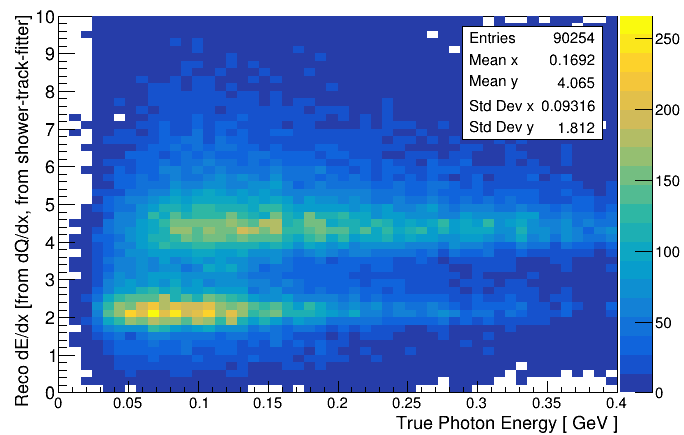
\includegraphics[width=1.00\textwidth]{egamma/dedx_vs_energy_gamma.png}
    \caption{\label{fig:dedxgammas:energy} d$E$/d$x$ vs. distance from shower start-point for $\gamma$ showers}
    \end{subfigure}
    \begin{subfigure}[b]{0.45\textwidth}
    \centering
    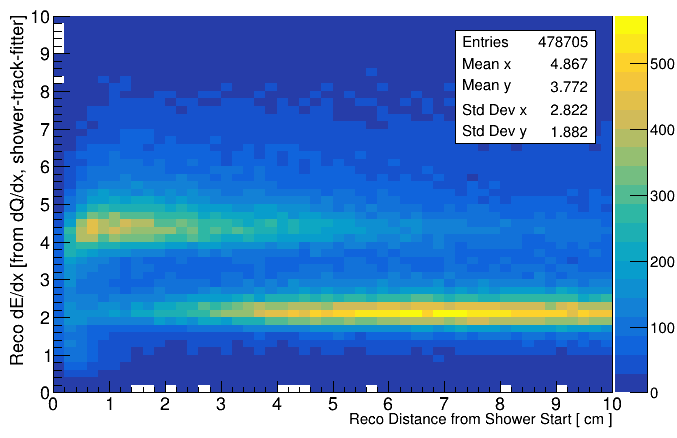
\includegraphics[width=1.00\textwidth]{egamma/dedx_vs_dist_gamma.png}
    \caption{\label{fig:dedxgammas:dist} d$E$/d$x$ vs. distance from shower start-point for $\gamma$ showers}
    \end{subfigure}
\caption{\label{fig:dedxgammas}}
\end{center}
\end{figure}



\newpage

\subsection{Energy Reconstruction \textcolor{red}{Giuseppe + David}}
\label{sec:ereco}
\par Energy reconstruction is performed calorimetrically for EM showers and through a measurement of a track's range for contained muons and protons. For muons multiple Coulomb scattering (MCS) is also used to estimate the muon energy. The energy resolution obtained for different particles is reported in table~\ref{tab:eres}. More information on each particle specie's energy resolution is reported in figure~\ref{fig:eres:particle} where for each particle species the 2D reconstructed vs. true energy distribution (in log-scale) is shown on the left, next to a plot of energy resolution vs. true energy on the right. The energy resolution reported here is obtained from a Gaussian plus one-sided exponential fit to the distribution $[E_{\rm reco}-E_{\rm true}] / E_{\rm true}$. The resolution reported refers only to the Gaussian width $\sigma$ extracted in the fit, and therefore does not account for negative tails, which are significant in the case of EM shower energy reconstruction, and described below.


\begin{table}[H]
\centering
  \begin{tabular}{ | c | c |  }
    \hline
    particle & kinetic energy resolution  \\ \hline
    proton & 4\% at 100 MeV 1\% at 200 MeV \\ \hline
    muon (range) & 3\%  \\ \hline
    muon (MCS) & $\frac{4.7\%}{\sqrt{E/{\rm GeV}}} \otimes \frac{2.8\%}{E/{\rm GeV}} \otimes 0.0\%$  \\ \hline
    electron & 15\%  \\
    \hline
    
  \end{tabular}
  \caption{\label{tab:eres} Energy resolution for different particle species.}
 \end{table}
 
 \par For EM showers, the calorimetric energy reconstruction response has a significant non-Gaussian component, as well as a large bias. Both effects are attributable to reconstruction effects associated with under-clustering of charge. The energy bias is found to be 20\% and approximately flat in energy, and motivates a definition of a corrected shower energy, defined as $E_{\rm corrected} = E_{\rm calorimetry} / 0.8$. The non-Gaussian response for EM energy reconstruction can be modeled through a Gaussian plus one-sided exponential distribution. Figure~\ref{fig:eres:elec:binned} shows in different bins of true energy the fractional energy response and a fit to a Gaussian plus one-sided exponential function. The residual energy bias, after the 20\% correction applied, is of order $3-8$\%. 
 
 \begin{figure}[ht]
\begin{center}
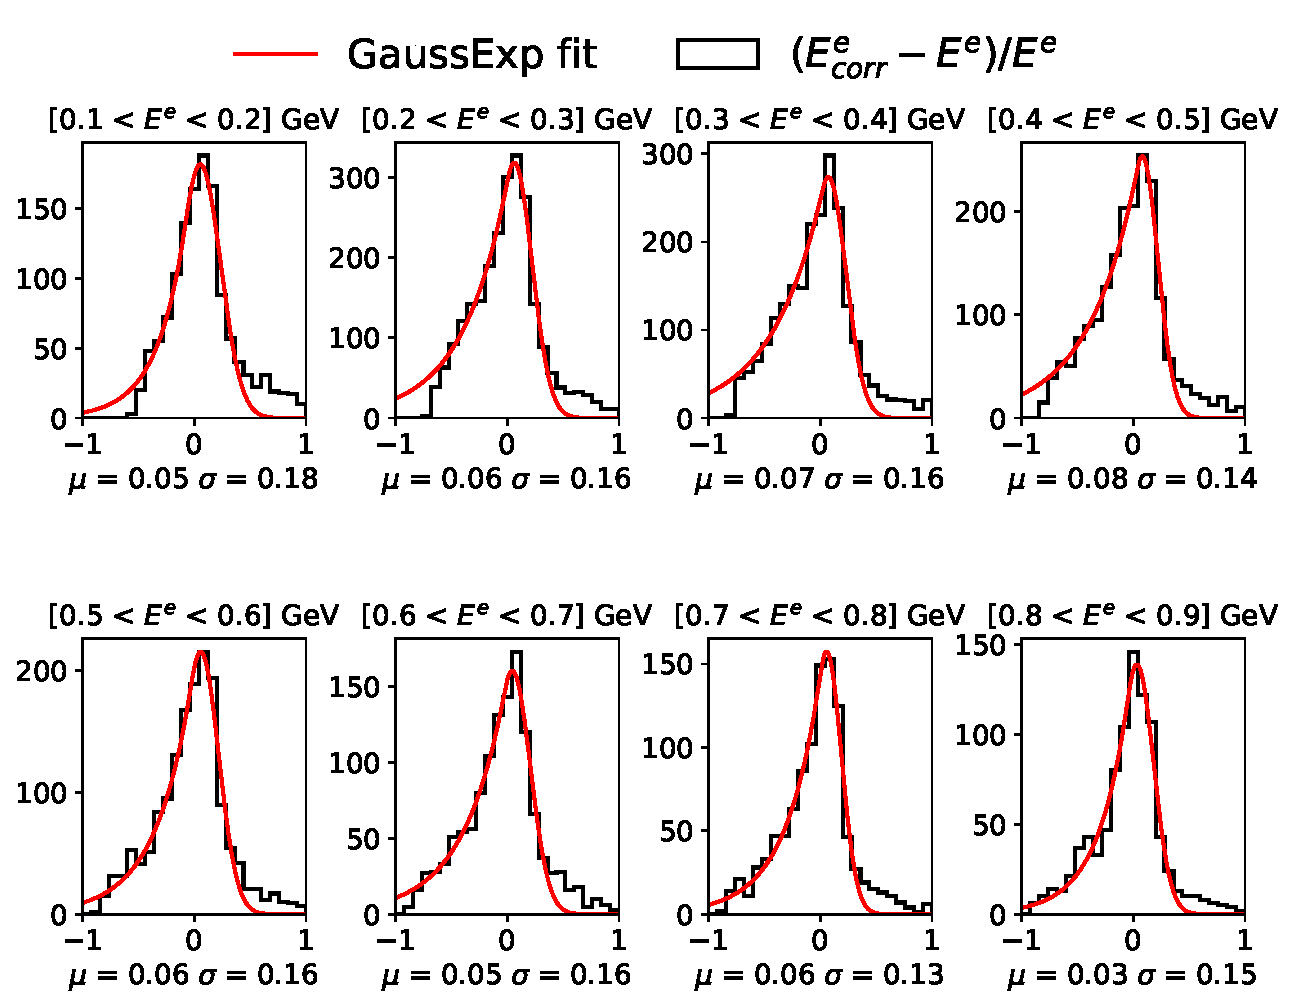
\includegraphics[width=0.75\textwidth]{ereco/elec_eres_binned.pdf}
\caption{\label{fig:eres:elec:binned}Energy resolution for electron showers.}
\end{center}
\end{figure}
 
 \newpage

\begin{figure}[H] 
\begin{center}
    \begin{subfigure}[b]{0.4\textwidth}
    \centering
    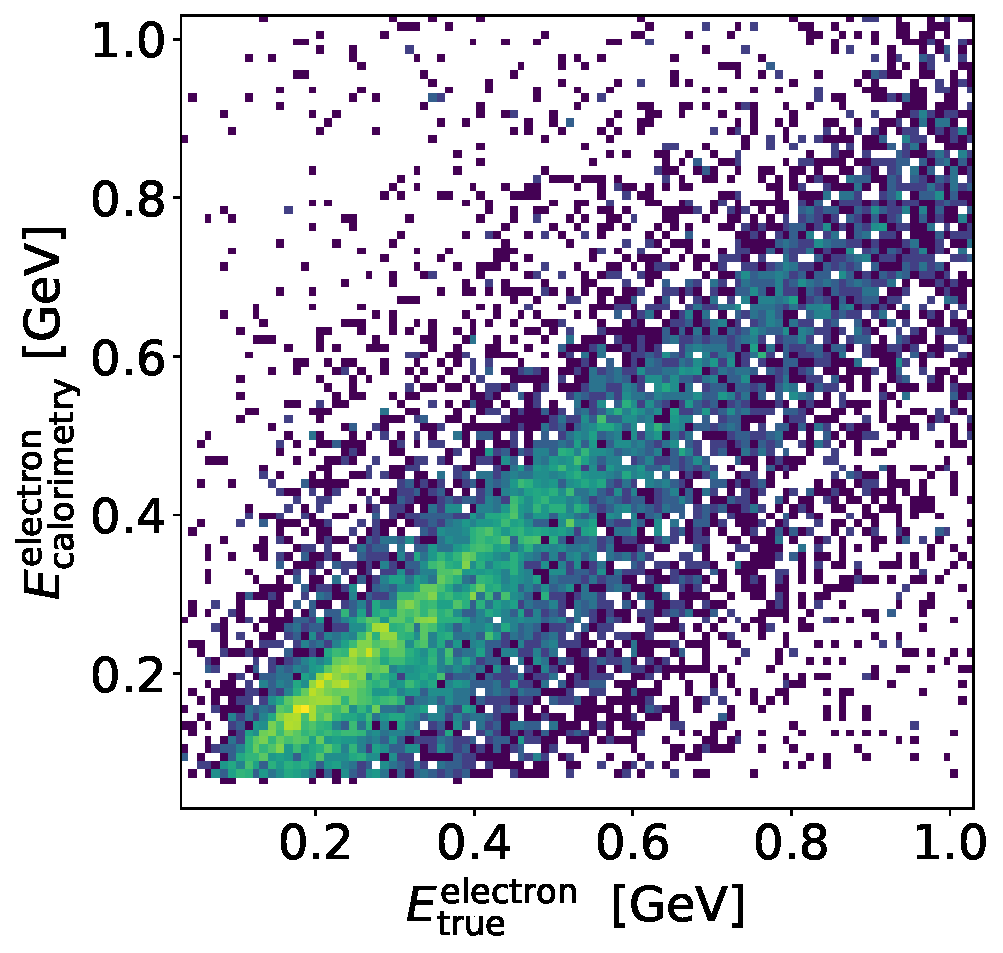
\includegraphics[width=1.00\textwidth]{ereco/electron_eres2D.pdf}
    %\caption{\label{fig:eres:elec:2d} }
    \end{subfigure}
    \begin{subfigure}[b]{0.38\textwidth}
    \centering
    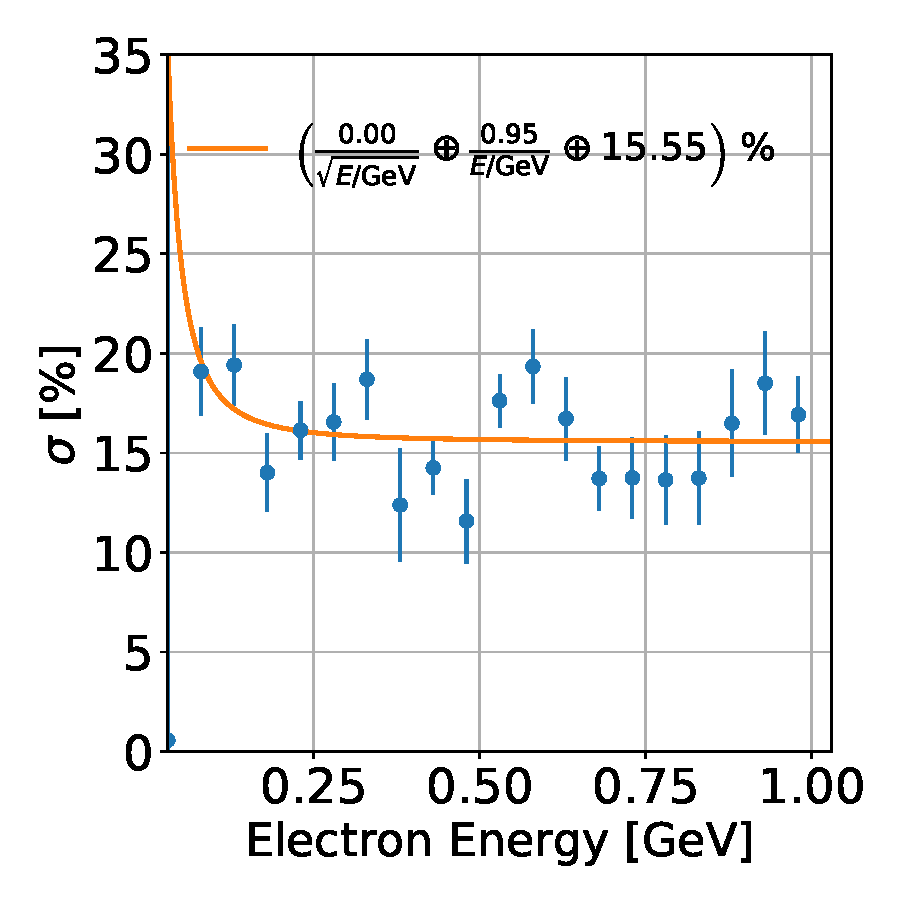
\includegraphics[width=1.00\textwidth]{ereco/elec_eres_vs_true.pdf}
    %\caption{\label{fig:eres:elec:vstrue} }
    \end{subfigure}
    \begin{subfigure}[b]{0.4\textwidth}
    \centering
    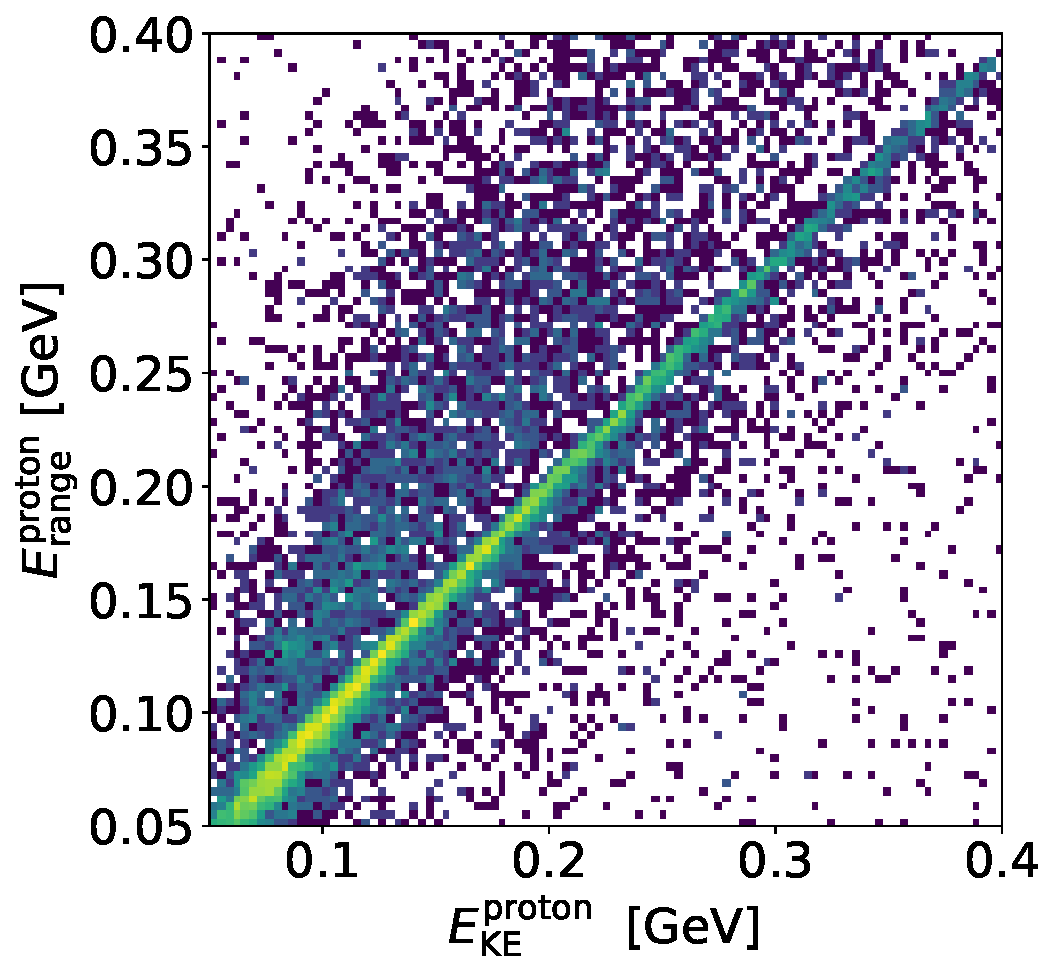
\includegraphics[width=1.00\textwidth]{ereco/proton_eres2D.pdf}
    %\caption{\label{fig:eres:proton:2d} }
    \end{subfigure}
    \begin{subfigure}[b]{0.38\textwidth}
    \centering
    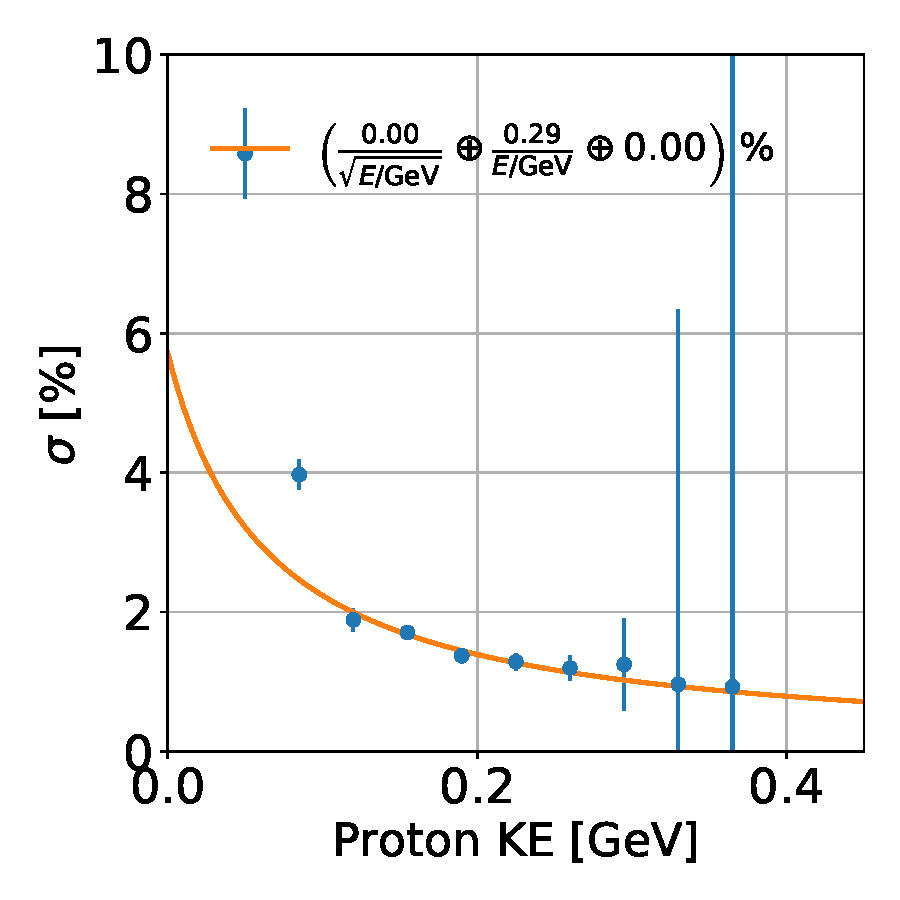
\includegraphics[width=1.00\textwidth]{ereco/proton_eres_vs_true.pdf}
    %\caption{\label{fig:eres:proton:vstrue} }
    \end{subfigure}
    \begin{subfigure}[b]{0.4\textwidth}
    \centering
    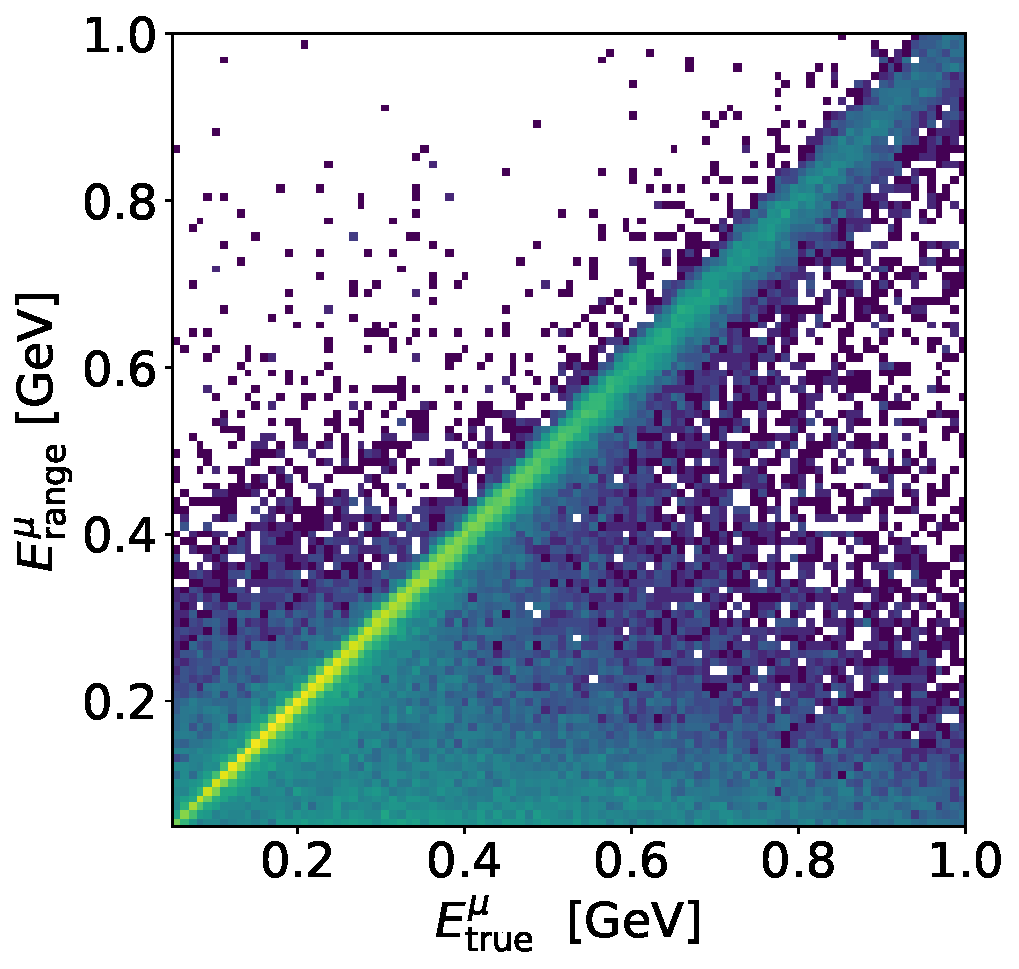
\includegraphics[width=1.00\textwidth]{ereco/muon_range_eres2D.pdf}
    %\caption{\label{fig:eres:muon:2d} }
    \end{subfigure}
    \begin{subfigure}[b]{0.38\textwidth}
    \centering
    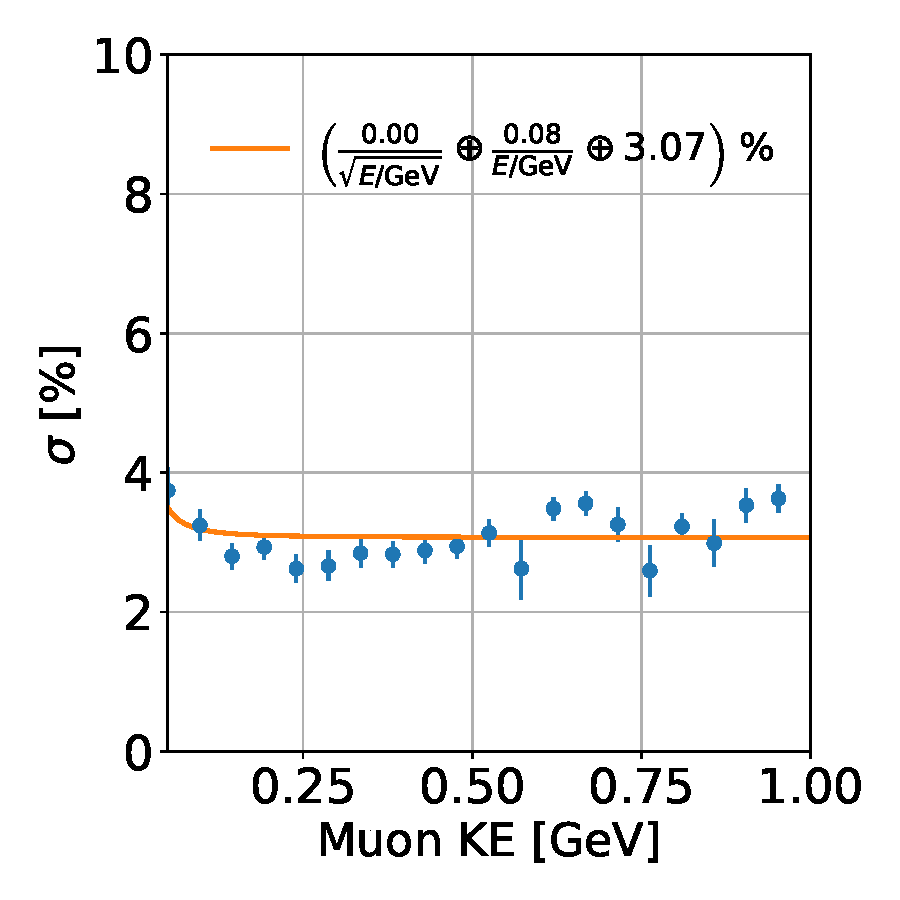
\includegraphics[width=1.00\textwidth]{ereco/muon_range_eres_vs_true.pdf}
    %\caption{\label{fig:eres:muon:vstrue} }
    \end{subfigure}
\caption{\label{fig:eres:particle}Energy resolution for electrons (top), protons (center) and muons (bottom). Left: reconstructed vs. true energy resolution (log-scale). Right: energy resolution from Gaussian fit to $[E_{\rm reco}-E_{\rm true}] / E_{\rm true}$.}
\end{center}
\end{figure}

\newpage

\subsubsection{Neutrino Energy Reconstruction}

\par In this analysis, the energy reconstruction for neutrino interactions is performed through a sum of the visible energy of the various reconstructed final-state particles in the interaction. For $\nu_e$ events the reconstructed energy is defined as:
\begin{equation}
    E_{\rm reco}^{\nu_e} = E_{\rm corrected}^{\rm electron} + \sum_{\rm tracks} E_{\rm range}^{\rm proton}
\end{equation}{}

For contained $\nu_{\mu}$ interactions, the reconstructed energy is defined as:

\begin{equation}
    E_{\rm reco}^{\nu_{\mu}} = E_{\rm range}^{\rm muon} + \sum_{\rm protons} E_{\rm range}^{\rm proton} + 0.105 \; GeV
\end{equation}{}

Figure~\ref{fig:eres:neutrino} shows the comparison between reconstructed energy and truth visible energy, which is defined as the sum of the lepton energy, pion energy (if present), and proton energy (for all protons above 40 MeV of KE). This comparison shows very accurate energy reconstruction for $\nu_{\mu}$ events. For $\nu_e$ interactions, with smearing dominated by the worse energy resolution of electron showers.

\begin{figure}[H] 
\begin{center}
    \begin{subfigure}[b]{0.4\textwidth}
    \centering
    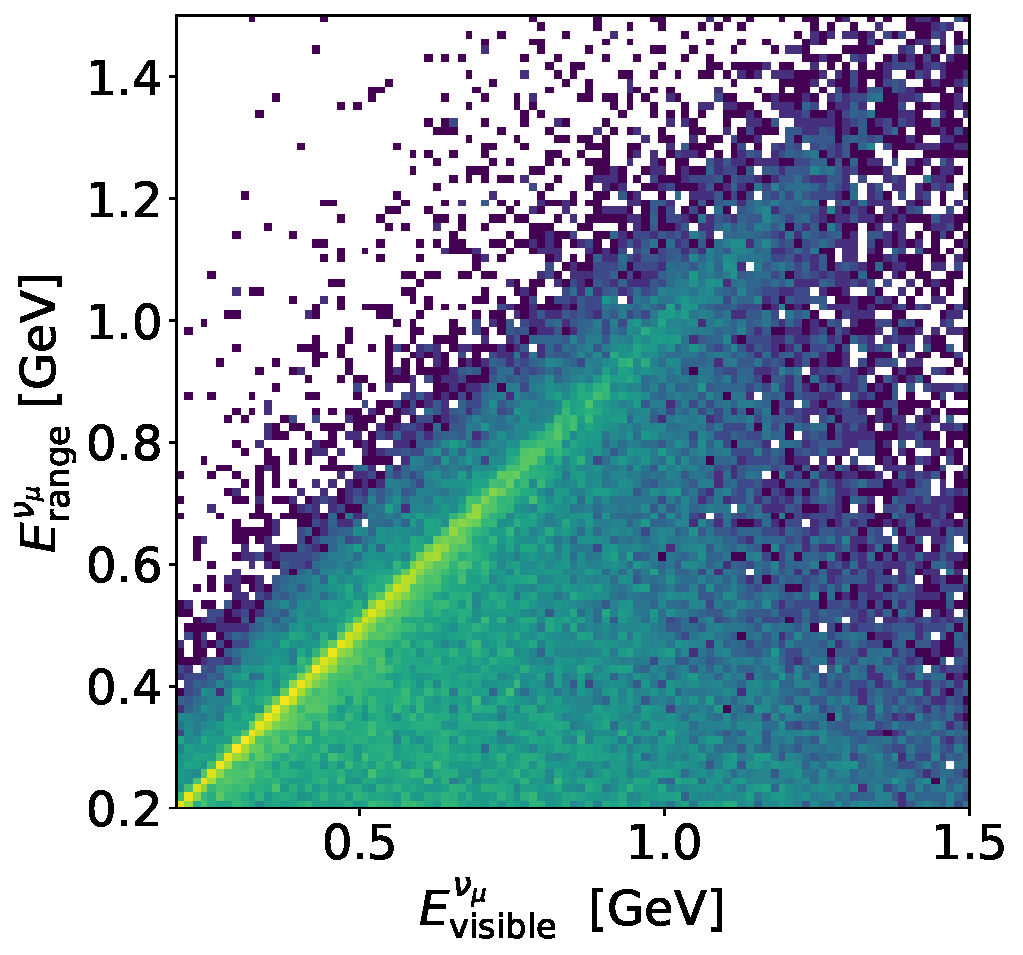
\includegraphics[width=1.00\textwidth]{ereco/numu_energy_visible_eres2D.pdf}
    \caption{\label{fig:eres:numu:2d} }
    \end{subfigure}
    \begin{subfigure}[b]{0.4\textwidth}
    \centering
    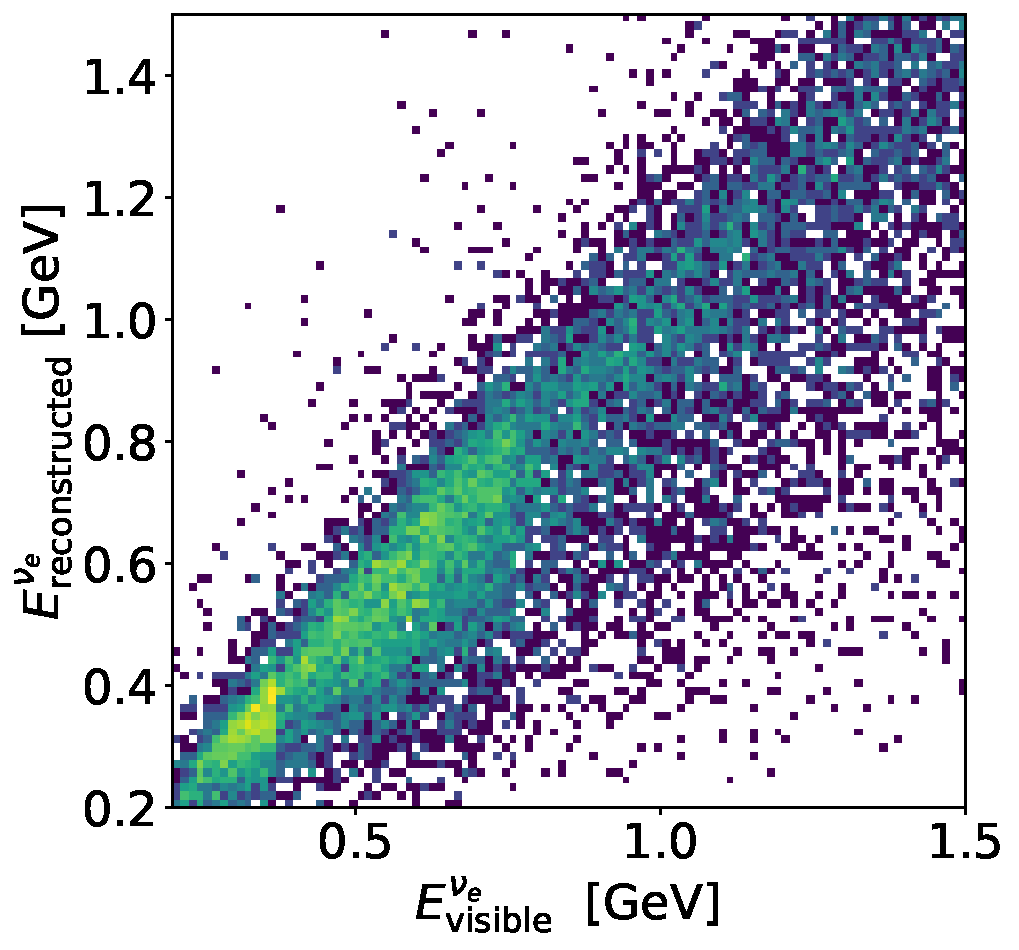
\includegraphics[width=1.00\textwidth]{ereco/nue_visible_eres2D.pdf}
    \caption{\label{fig:eres:nue:vstrue} }
    \end{subfigure}
\caption{\label{fig:eres:neutrino}Log-scale color-maps.}
\end{center}
\end{figure}

\newpage

\section{Control Samples and Analysis Input Validation}
\par The selections and analysis described below rely on well understood detector, simulation, calibration, and analysis tools performance. This section is dedicated to providing information pertaining to the robustness of the analysis developed. 
\par It is important to note that in addition to detector simulation and reconstruction effects, $\nu$-Ar modeling can impact the level of data-mc agreement in various variables. We will try to point out when this might be the case.
\subsection{$\pi^0$ control sample}
\par A $\pi^0$ selection has been developed in order to obtain high-stats samples of $\pi^0$ events and $\gamma$ EM showers which can constrain $\pi^0$ production modeling uncertainties as well as validate the analyis' ability to reconstruct and select EM showers.
\par Figure~\ref{fig:pi0:mass} shows the reconstructed $M\gamma\gamma$ for candidate $\pi^0$ events, with a calibrated but uncorrected (i.e. not accounting for biases in shower energy reconstruction caused by the incompleteness in charge clustering) energy reconstruction. Overall there is good data-MC agreement, apart from an apparent normalization difference. To account for this normalization difference we measure a flat scaling factor needed for CC and NC $\pi^0$ events needed to obtain  consitent rate in data and MC. This factor is found to be 72.4\% in Run1 and 72.7\% in Run3. We repeat the exercise applying a tighter $\pi^0$ selection enhancing the $\pi^0$ purity and obtain scaling factors of 70\% for both Run1 and Run3. While this procedure is far from rigorous, it allows us to study detector-related and specifically shower-related variables removing a large normalization difference. \textcolor{red}{A more rigorous data-driven constrain of our $\pi^0$ rate, performed accounting for detector and flux systematics, and considering a broader range of $\pi^0$ modeling, will need to be performed.}

\begin{figure}[H] 
\begin{center}
    \begin{subfigure}[b]{0.3\textwidth}
    \centering
    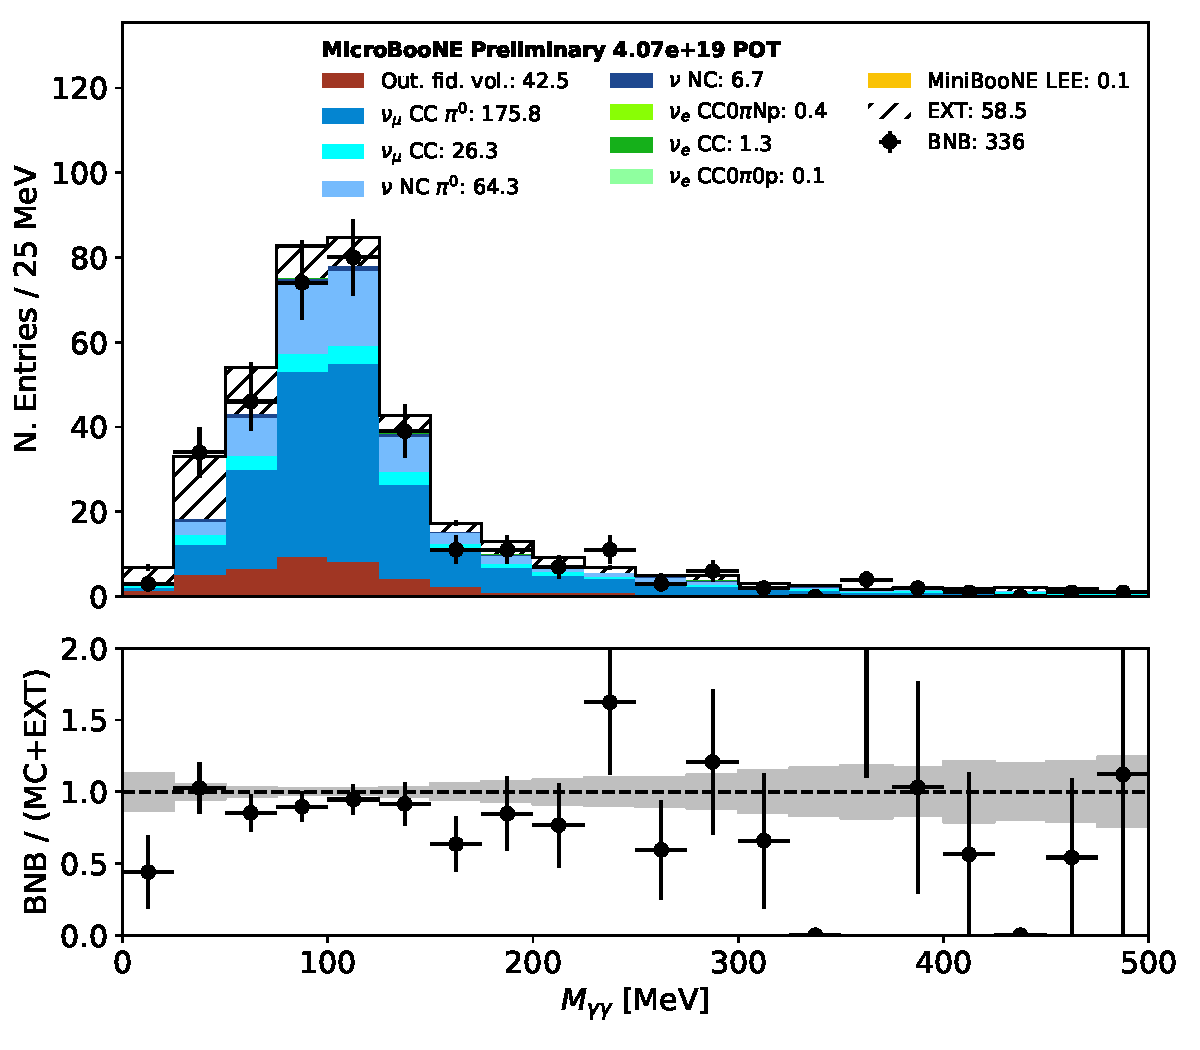
\includegraphics[width=1.00\textwidth]{pi0/pi0_mass_Y_01142020_5E19.pdf}
    \caption{\label{fig:pi0:mass:5E19} Run 1 ``5E19'' open dataset.}
    \end{subfigure}
    \begin{subfigure}[b]{0.3\textwidth}
    \centering
    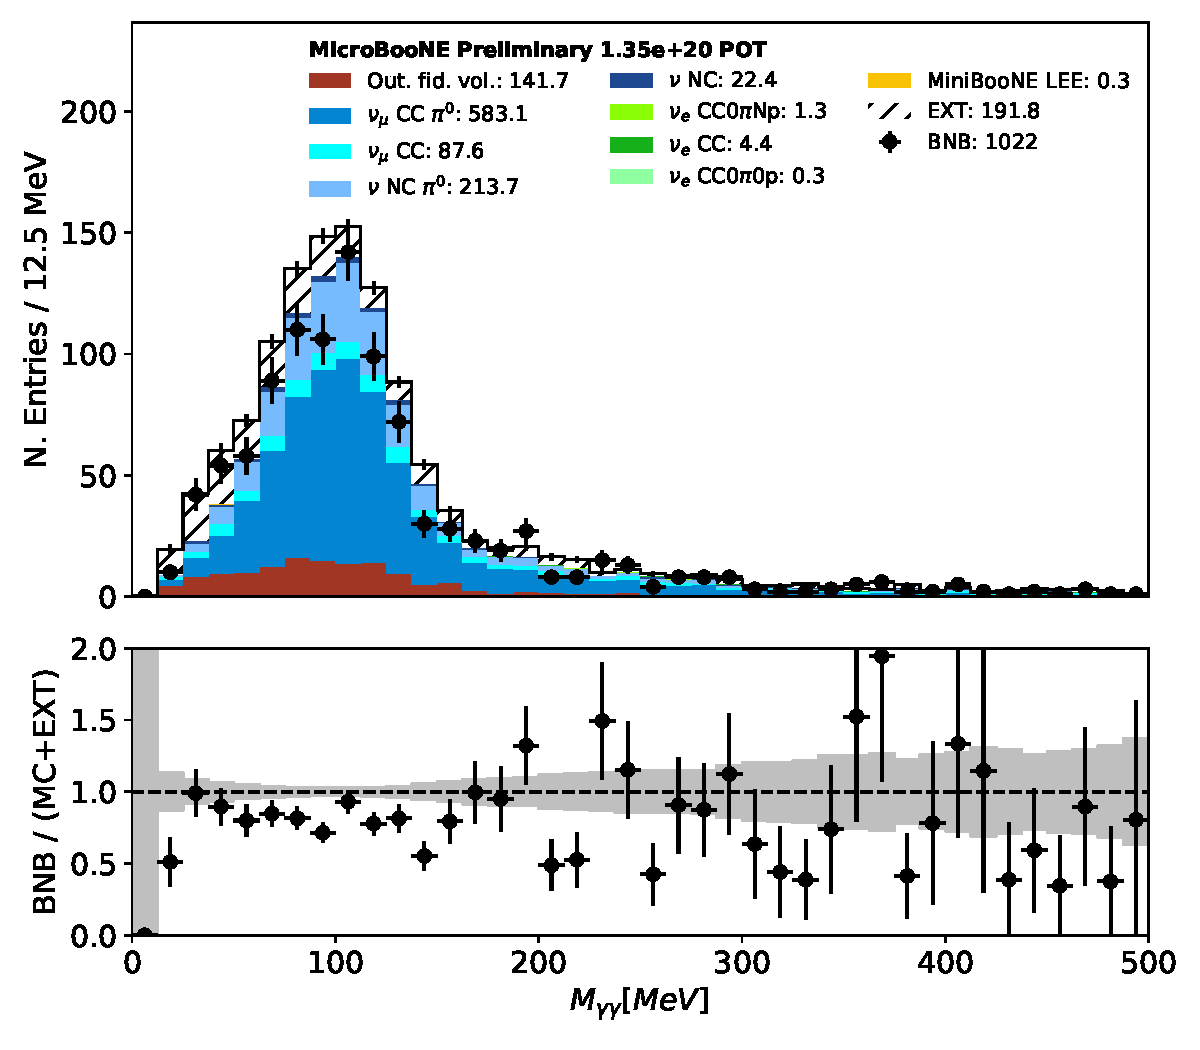
\includegraphics[width=1.00\textwidth]{pi0/pi0_mass_Y_01142020sel__RUN1.pdf}
    \caption{\label{fig:pi0:mass:5E19} Run 1.}
    \end{subfigure}
    \begin{subfigure}[b]{0.3\textwidth}
    \centering
    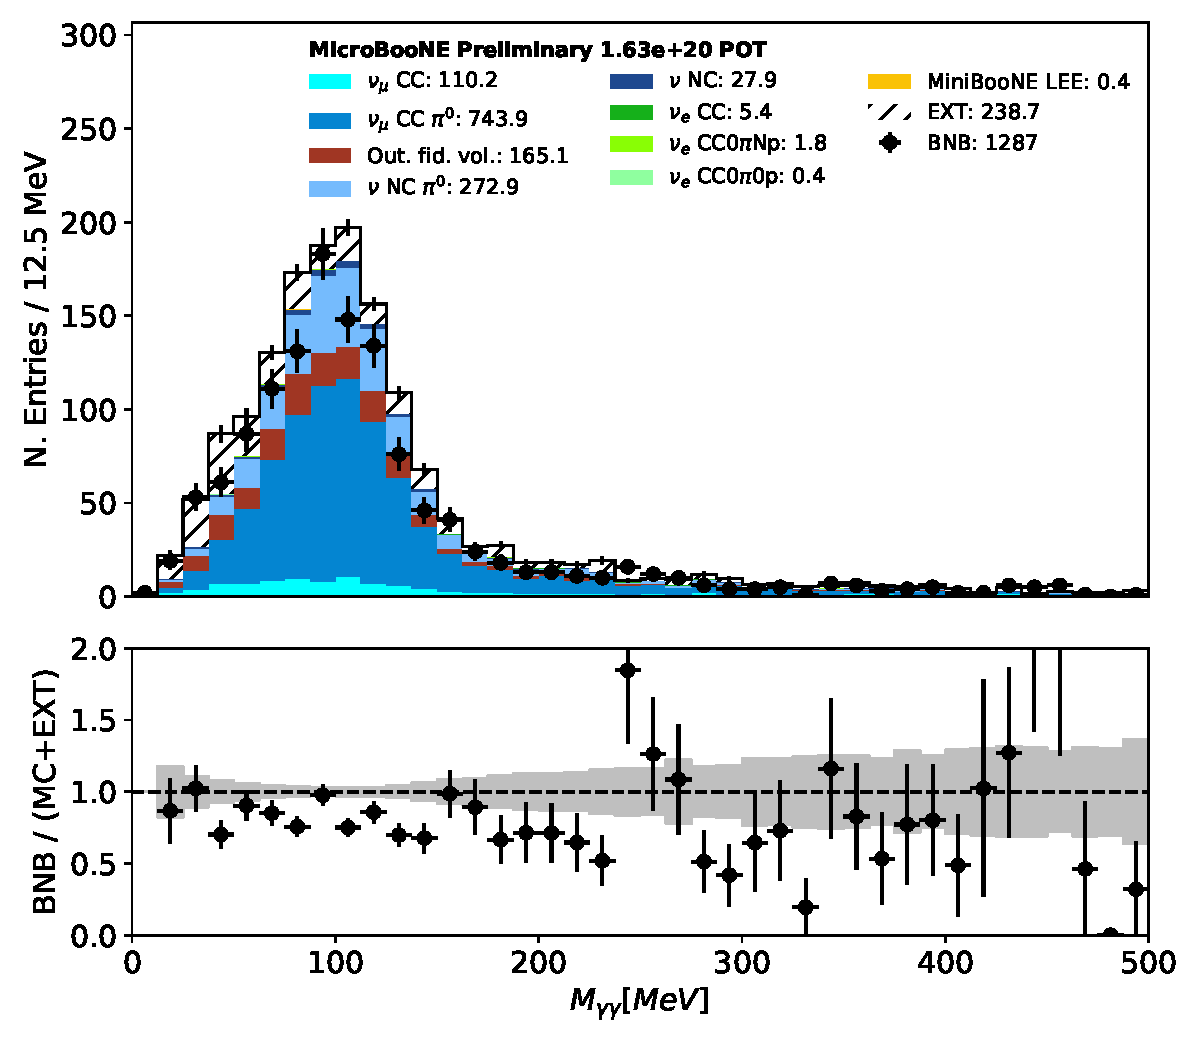
\includegraphics[width=1.00\textwidth]{pi0/pi0_mass_Y_01142020sel_RUN3.pdf}
    \caption{\label{fig:pi0:mass:5E19} Run 3.}
    \end{subfigure}
\caption{\label{fig:pi0:mass}Reconstructed $\pi^0$ mass.}
\end{center}
\end{figure}

\par After applying a scaling factor of 0.7 to CC and NC $\pi^0$ events in the MC, we show comparisons of shower variables with the goal of assessing data-mc agreement for the $\nu_e$ selection. Figure~\ref{fig:pi0:datamc} shows reconstructed quantities used in the $\nu_e$ analysis for $\pi^0$ candidate events which are useful in validating the rubstness of shower modeling. They include leading and sub-leading shower dE/dx (top), followed by the leading and sub-leading shower conversion distance and shower score. The last row reports the reconstructed shower Moliere angle and track PID score for the longest track in each event. Generally, the data-MC agreement is quite good. For d$E$/d$x$ there appears to be a clear distortion, specifically in the 4 MeV/cm peak associated with photons. \textcolor{red}{A re-calibration of shower d$E$/d$x$ is planned for the analysis, but has not been fully implemented as of now.}

\begin{figure}[H] 
\begin{center}
    \begin{subfigure}[b]{0.38\textwidth}
    \centering
    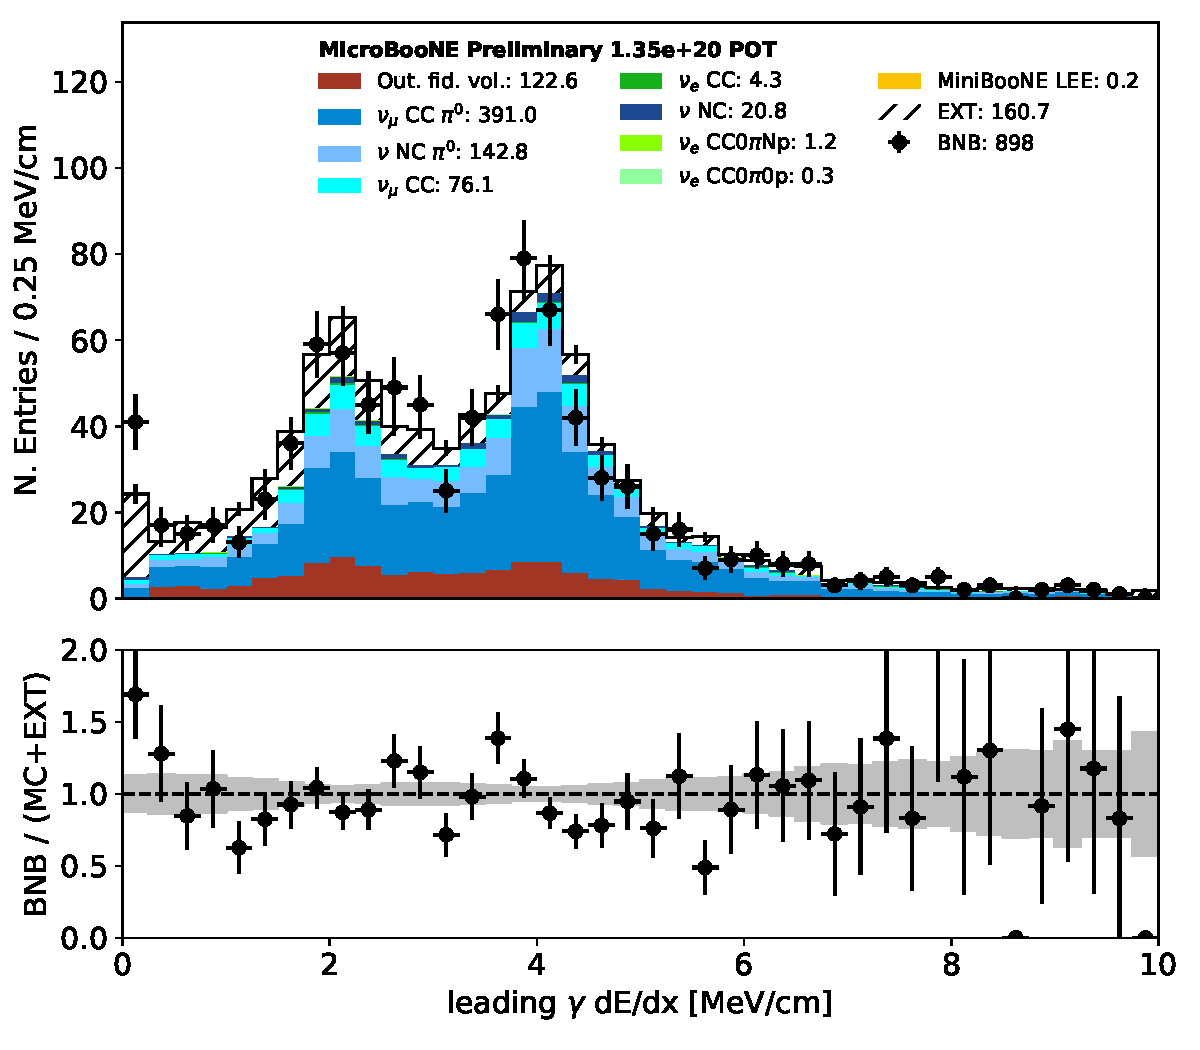
\includegraphics[width=1.00\textwidth]{pi0/pi0_dedx1_fit_Y_01152020_scaled_RUN1.pdf}
    %\caption{\label{fig:pi0:dedx:RUN1:leading} Run 1 leading shower.}
    \end{subfigure}
    \begin{subfigure}[b]{0.38\textwidth}
    \centering
    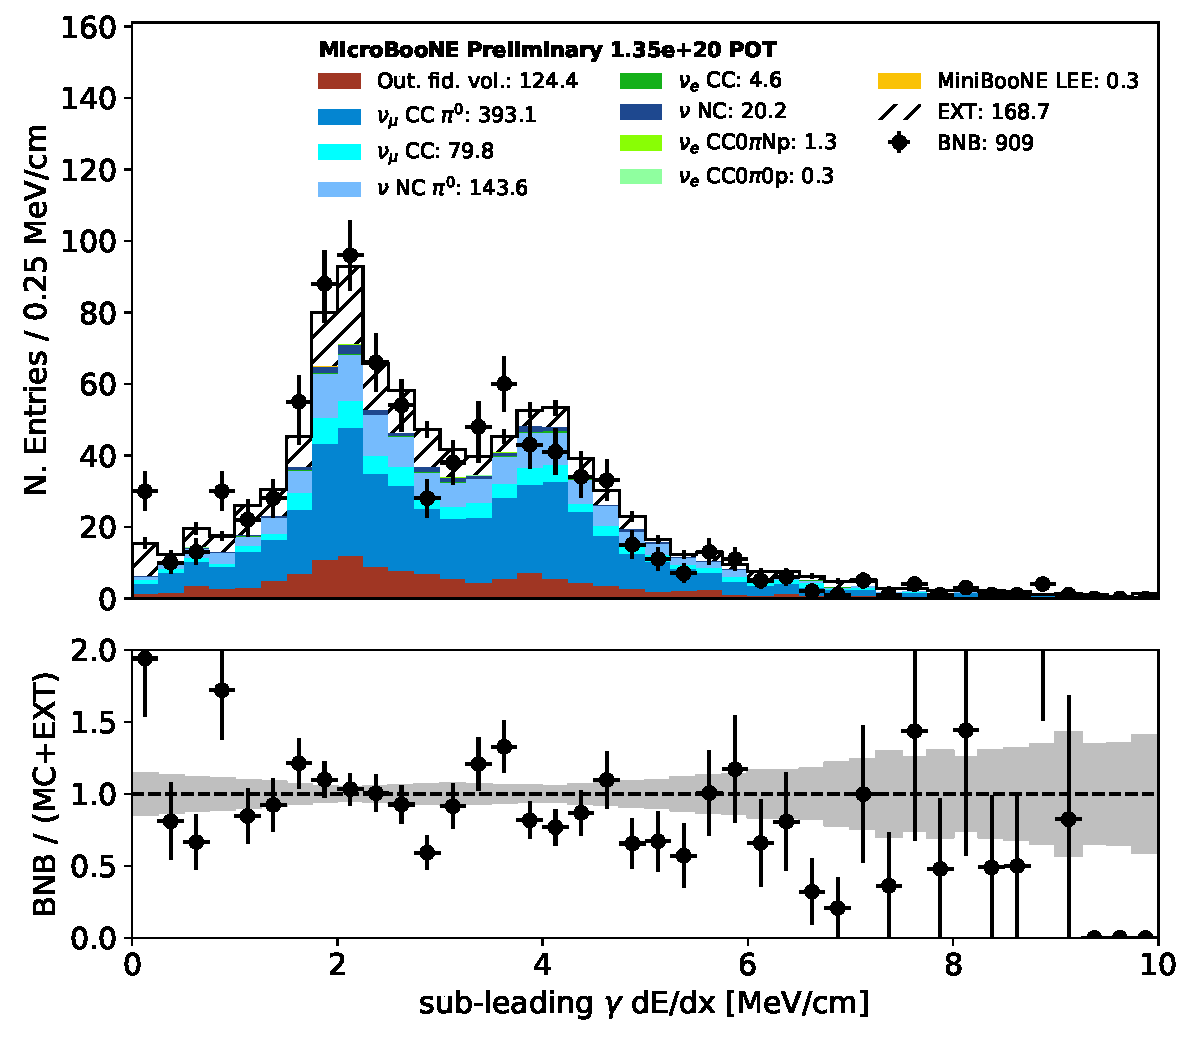
\includegraphics[width=1.00\textwidth]{pi0/pi0_dedx2_fit_Y_01152020_scaled_RUN1.pdf}
    %\caption{\label{fig:pi0:dedx:RUN1:subleading} Run 1 sub-leading shower.}
    \end{subfigure}
    
    \begin{subfigure}[b]{0.38\textwidth}
    \centering
    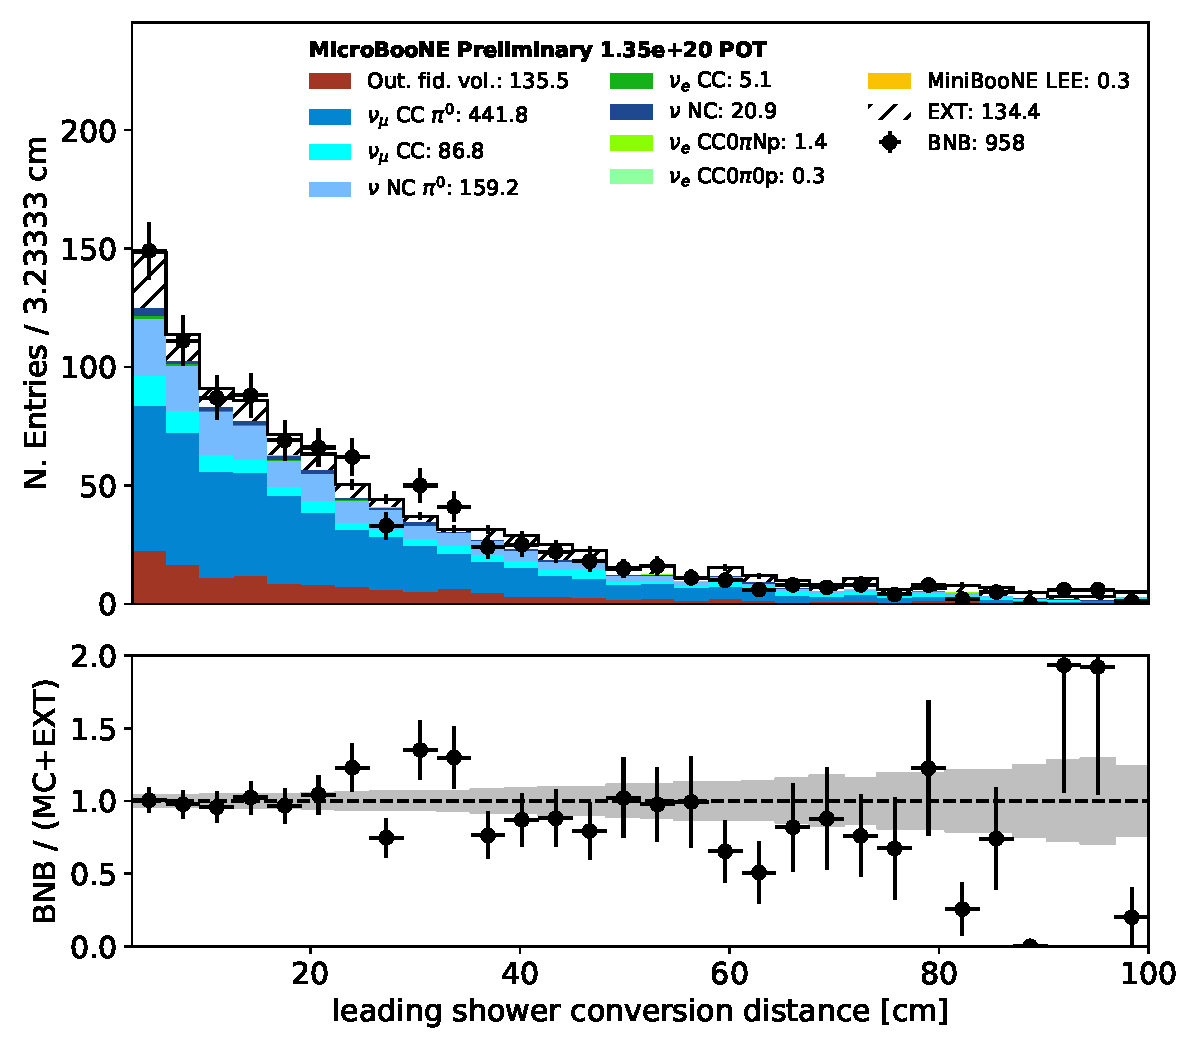
\includegraphics[width=1.00\textwidth]{pi0/pi0_radlen1_01152020_inputs_RUN1.pdf}
    %\caption{\label{fig:pi0:dedx:RUN1:leading} Run 1 leading shower.}
    \end{subfigure}
    \begin{subfigure}[b]{0.38\textwidth}
    \centering
    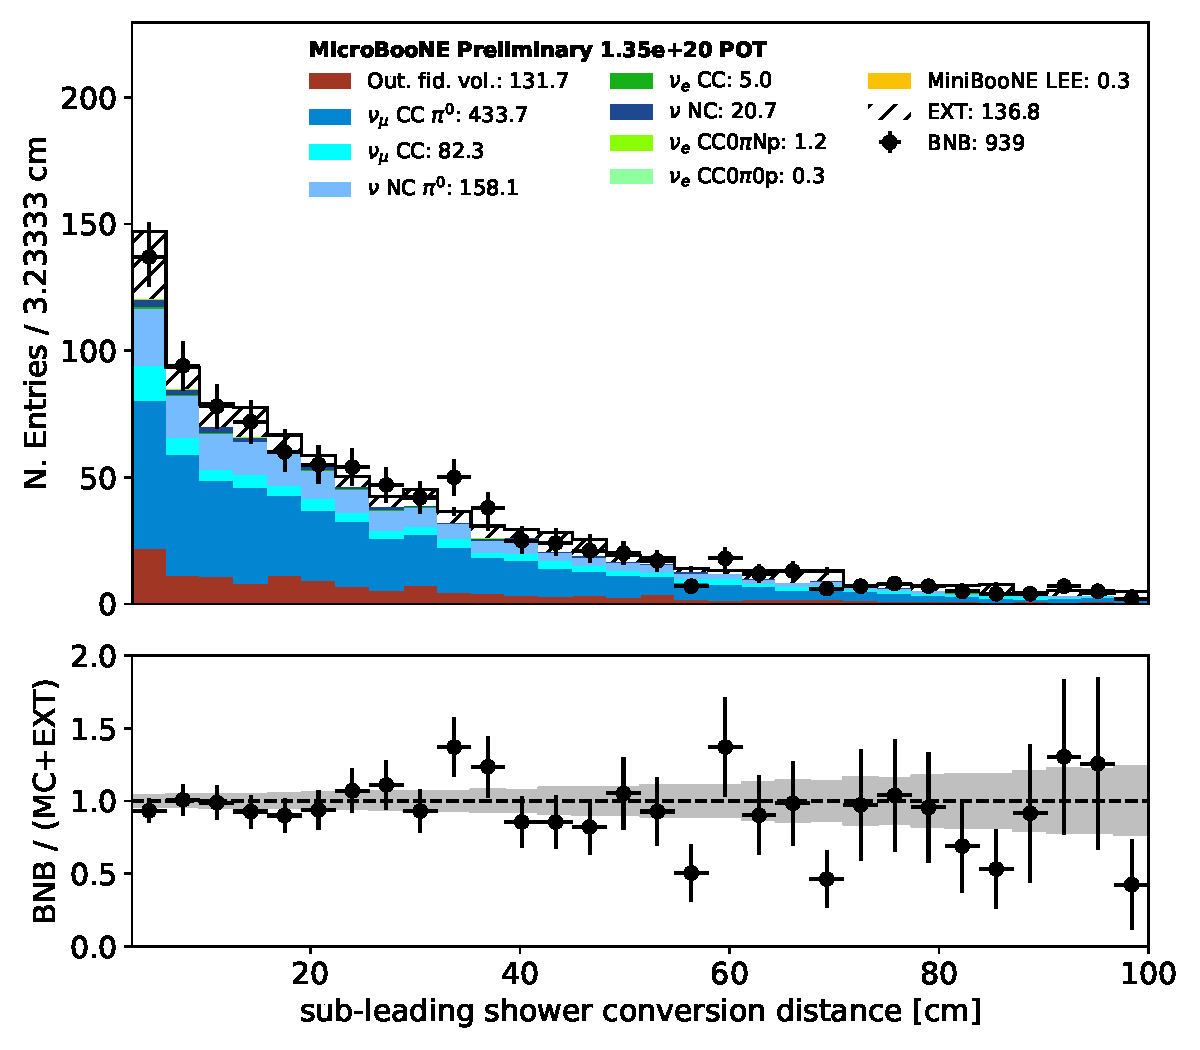
\includegraphics[width=1.00\textwidth]{pi0/pi0_radlen2_01152020_inputs_RUN1.pdf}
    %\caption{\label{fig:pi0:dedx:RUN1:subleading} Run 1 sub-leading shower.}
    \end{subfigure}
    
    \begin{subfigure}[b]{0.38\textwidth}
    \centering
    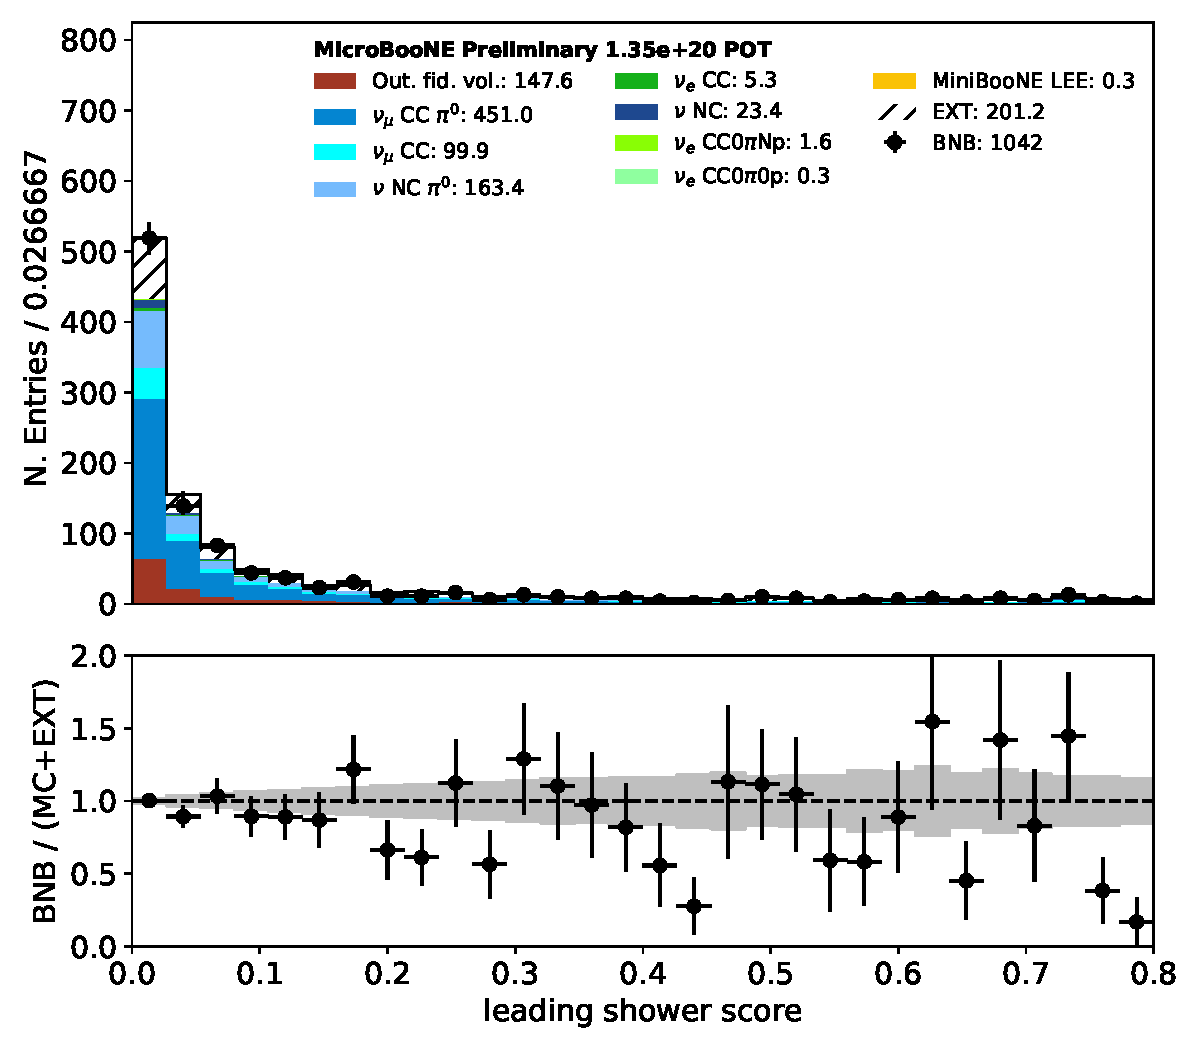
\includegraphics[width=1.00\textwidth]{pi0/pi0_shrscore1_01152020_inputs_RUN1.pdf}
    %\caption{\label{fig:pi0:dedx:RUN1:leading} Run 1 leading shower.}
    \end{subfigure}
    \begin{subfigure}[b]{0.38\textwidth}
    \centering
    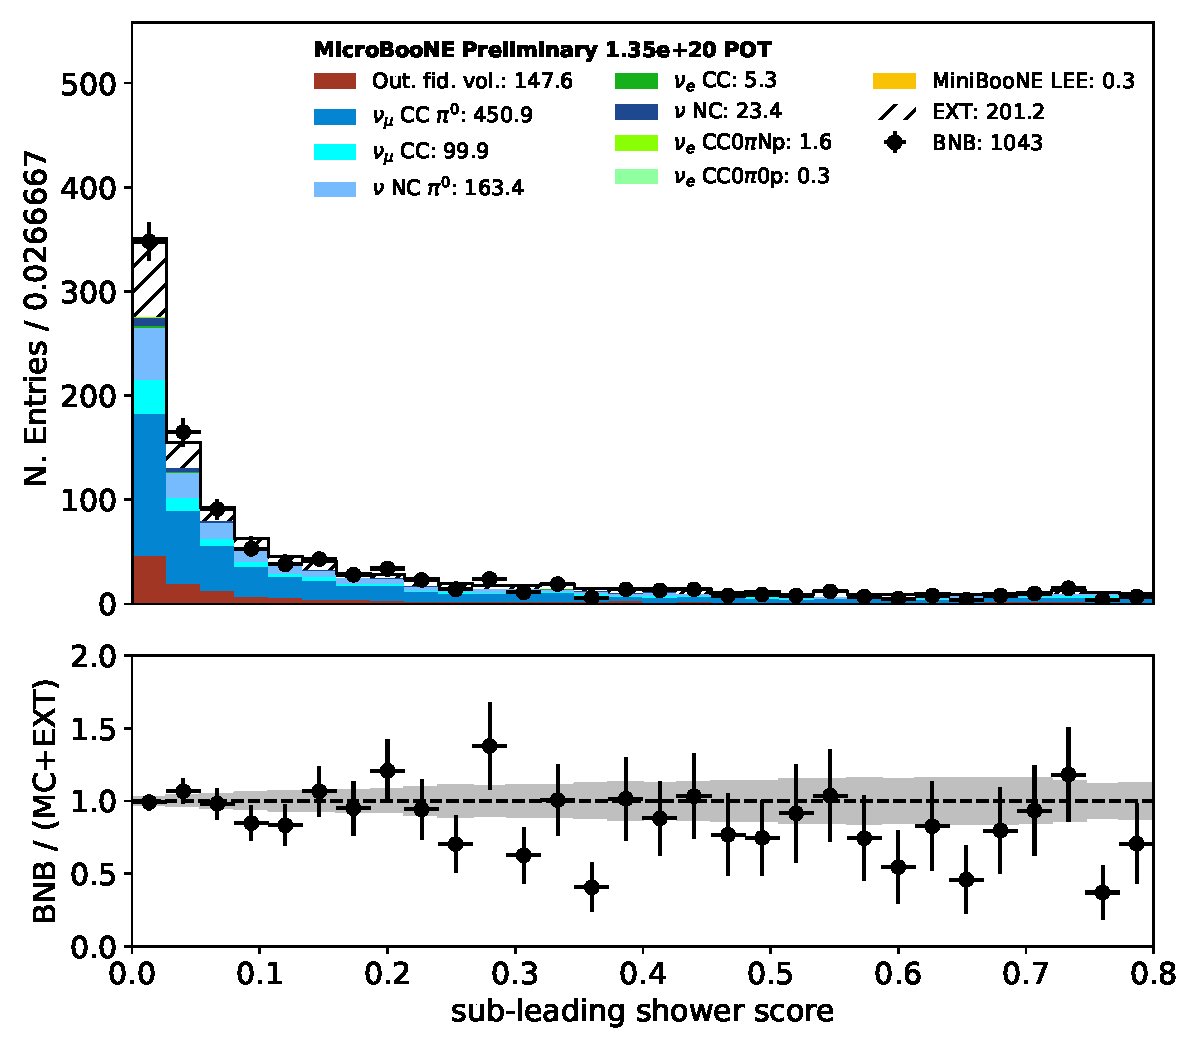
\includegraphics[width=1.00\textwidth]{pi0/pi0_shrscore2_01152020_inputs_RUN1.pdf}
    %\caption{\label{fig:pi0:dedx:RUN1:subleading} Run 1 sub-leading shower.}
    \end{subfigure}
    
    \begin{subfigure}[b]{0.38\textwidth}
    \centering
    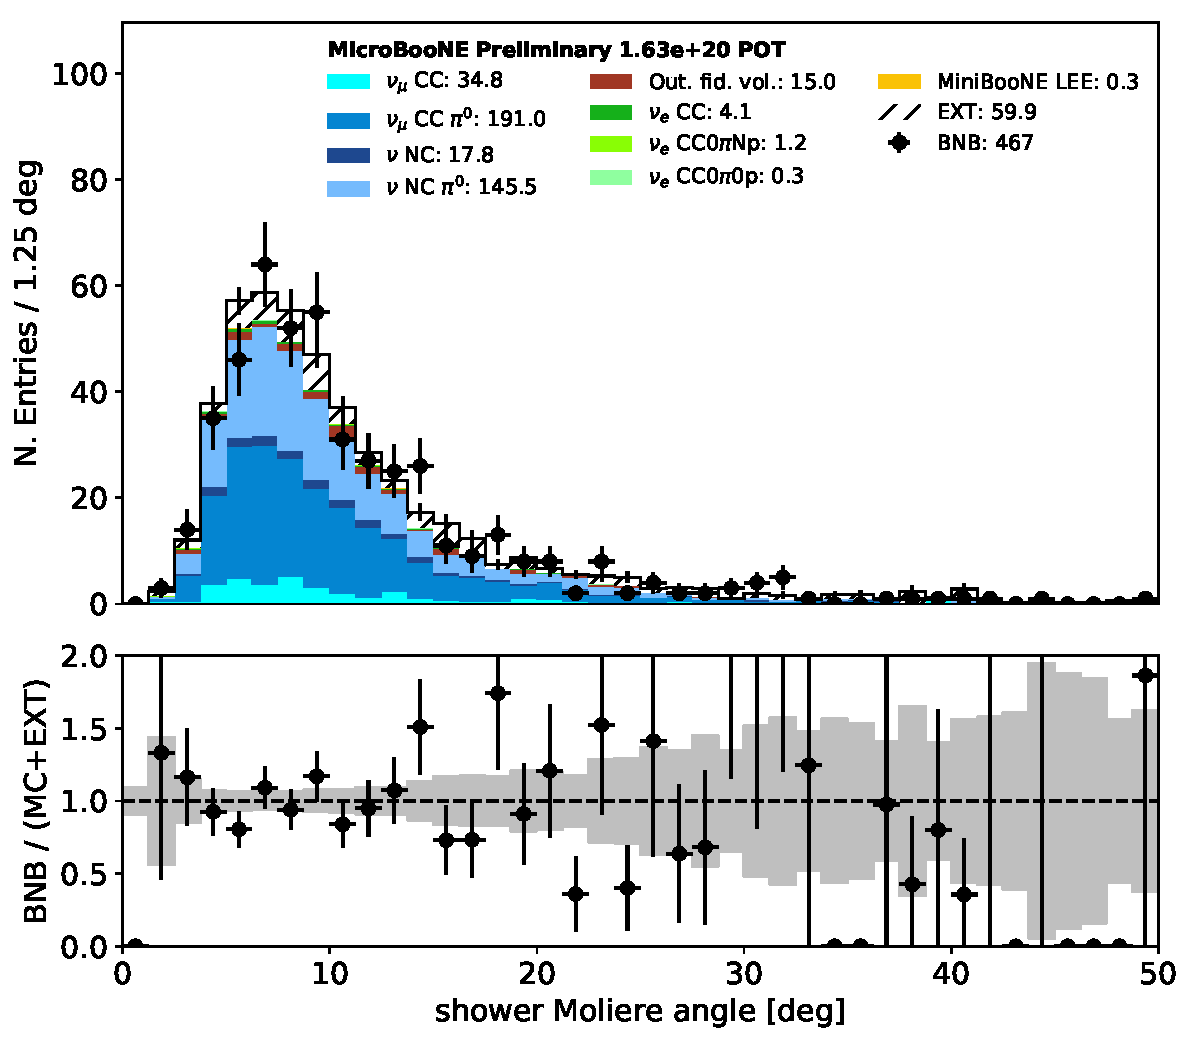
\includegraphics[width=1.00\textwidth]{pi0/shrmoliereavg_01152020_scaled_RUN3.pdf}
    %\caption{\label{fig:pi0:dedx:RUN1:leading} Run 1 leading shower.}
    \end{subfigure}
    \begin{subfigure}[b]{0.38\textwidth}
    \centering
    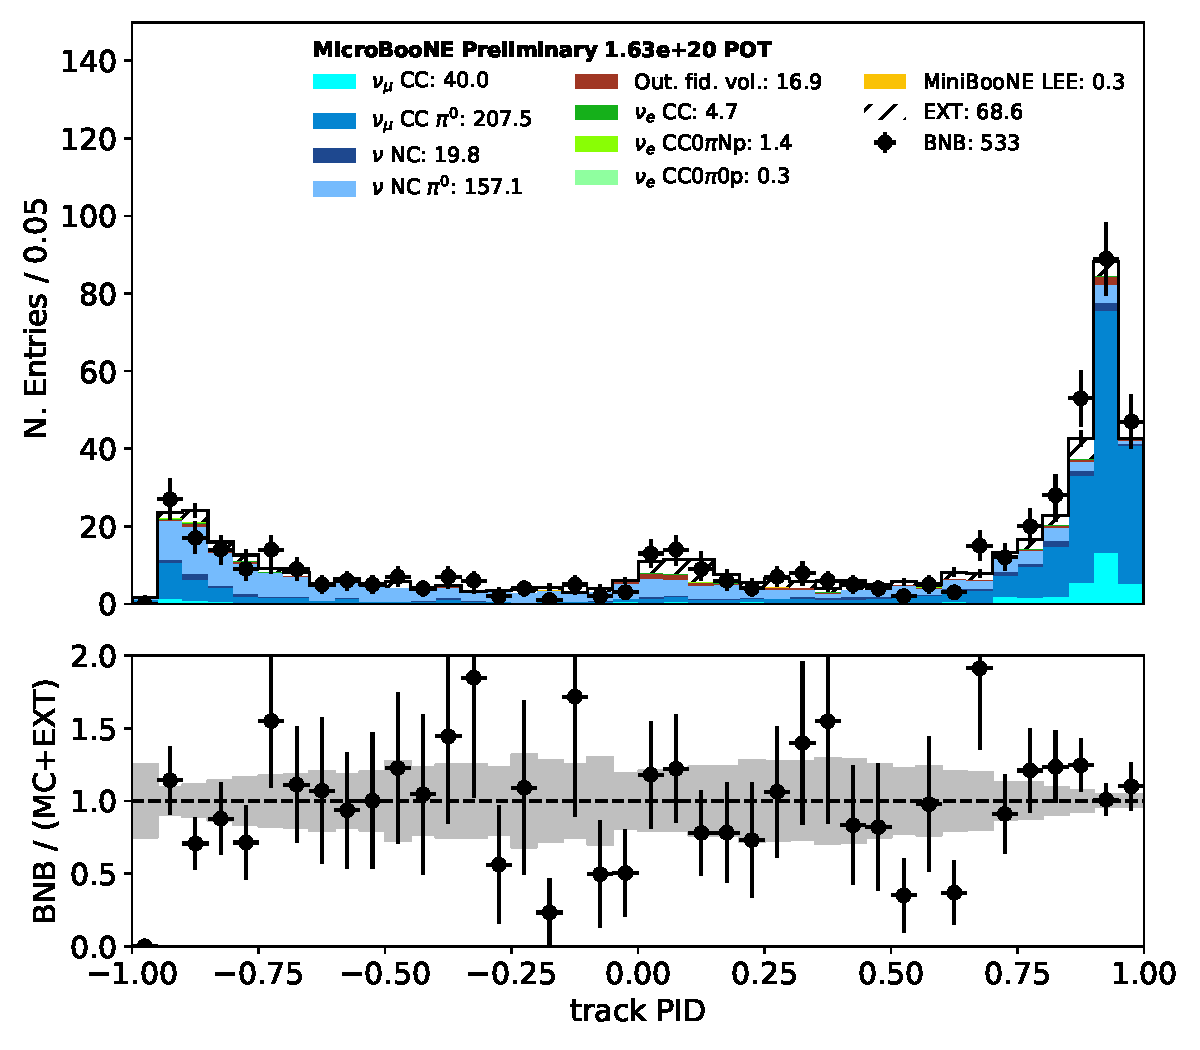
\includegraphics[width=1.00\textwidth]{pi0/trkpid_01152020_scaled_RUN3.pdf}
    %\caption{\label{fig:pi0:dedx:RUN1:subleading} Run 1 sub-leading shower.}
    \end{subfigure}
    
\caption{\label{fig:pi0:datamc}Reconstructed d$E$/d$x$ for leading and sub-leading showers.}
\end{center}
\end{figure}


\newpage

\section{$\nu_e$ Selections}
\par This chapter present the three $\nu_e$ selections which comprise the analysis. The starting point for the $\nu_e$ selections, including a description of efficiencies, are described in section~\ref{sec:nueselection:inputs} . The common variables and tools leveraged for the $\nu_e$ selection are presented in section~\ref{sec:nueselection:variables}. Following sections describe the three channels being targeted: $\nu_e$ inclusive (\ref{sec:nueselection:inclusive}),1$e$N$p$0$\pi$ (\ref{sec:nueselection:1eNp}), and 1$e$0$p$0$\pi$ (\ref{sec:nueselection:1e0p}).

\subsection{Input to $\nu_e$ selections and 1$e$N$p$/1$e$0$p$ orthogonality \textcolor{red}{Sophie + ...}}
\label{sec:nueselection:inputs}

The 1$e$N$p$ and 1$e$0$p$ selections rely on a common pre-selection which requires the presence of at least one reconstructed and contained EM shower (figure~\ref{fig:nue:presel:nshower}) with reconstructed energy above 70 MeV (figure~\ref{fig:nue:presel:shrenergy}). This second cut applies as a Michel-electron veto, as the majority of events which do not pass this cut are associated to cosmic or $\nu_{\mu}$ induced $\mu \rightarrow e$ Michel electrons. The two selections are subsequently split based on whether a proton candidate is (N$p$) or is not (0$p$) found. Events with a fully contained track must have a \texttt{trkpid} score $< 0$ and a value of \texttt{tksh\_angle} $> -0.9$. The first condition requires that the track be proton-like according to the PID tool~\ref{subsec:loglikelihoodpid}, while the second excludes tracks reconstructed back-to-back to the electron candidate, generally due to mis-reconstruction. For events with more than one reconstructed track, these requirements are applied on the longest track.

\begin{figure}[H] 
\begin{center}
    \begin{subfigure}[b]{0.3\textwidth}
    \centering
    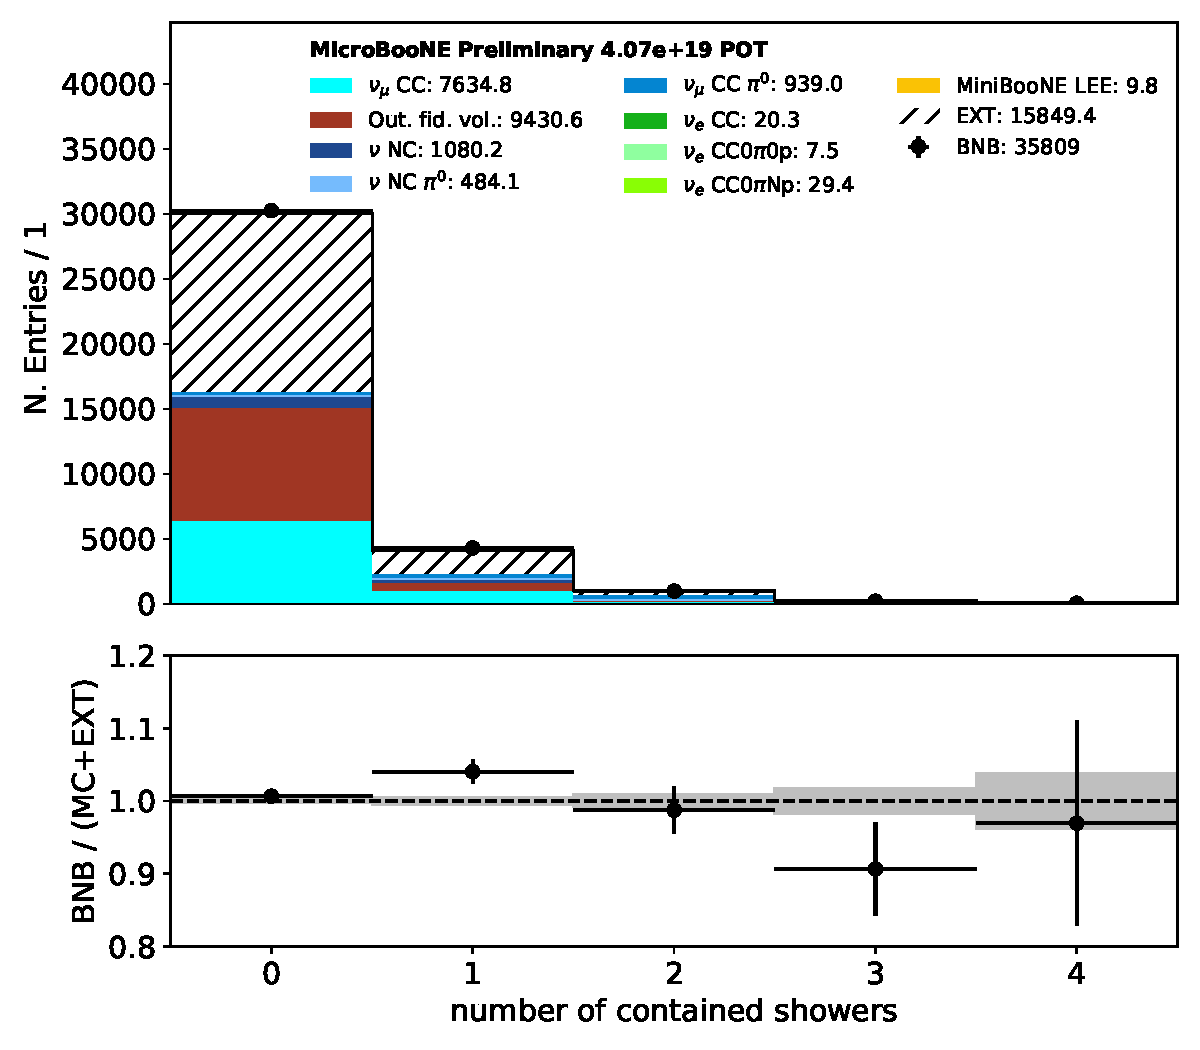
\includegraphics[width=1.00\textwidth]{nueselection/n_showers_contained_01132020_RUN1.pdf}
    \caption{\label{fig:nue:presel:nshower} }
    \end{subfigure}
    \begin{subfigure}[b]{0.3\textwidth}
    \centering
    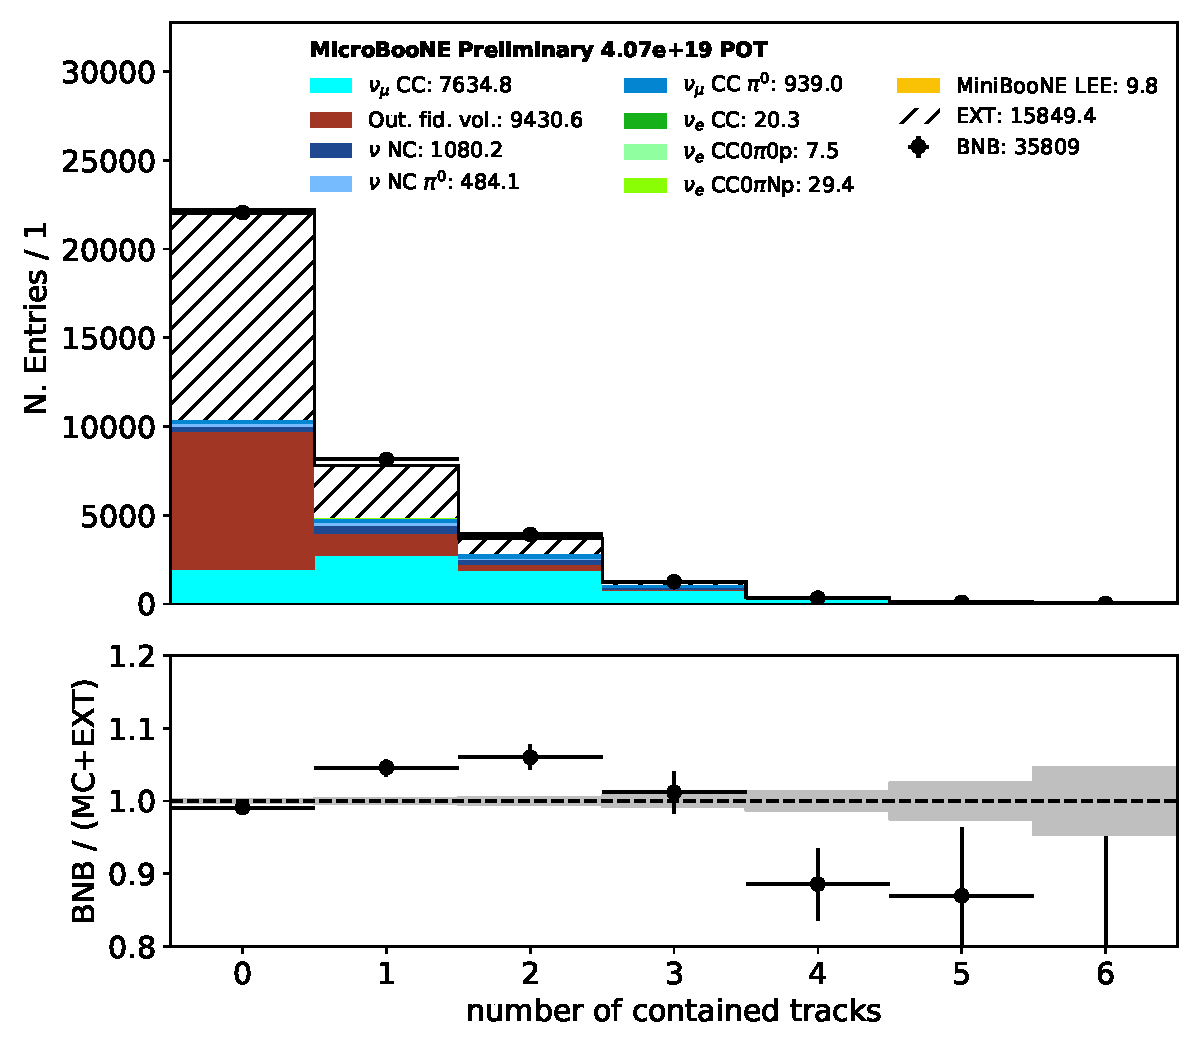
\includegraphics[width=1.00\textwidth]{nueselection/n_tracks_contained_01132020_RUN1.pdf}
    \caption{\label{fig:nue:presel:ntrack} }
    \end{subfigure}
    \begin{subfigure}[b]{0.3\textwidth}
    \centering
    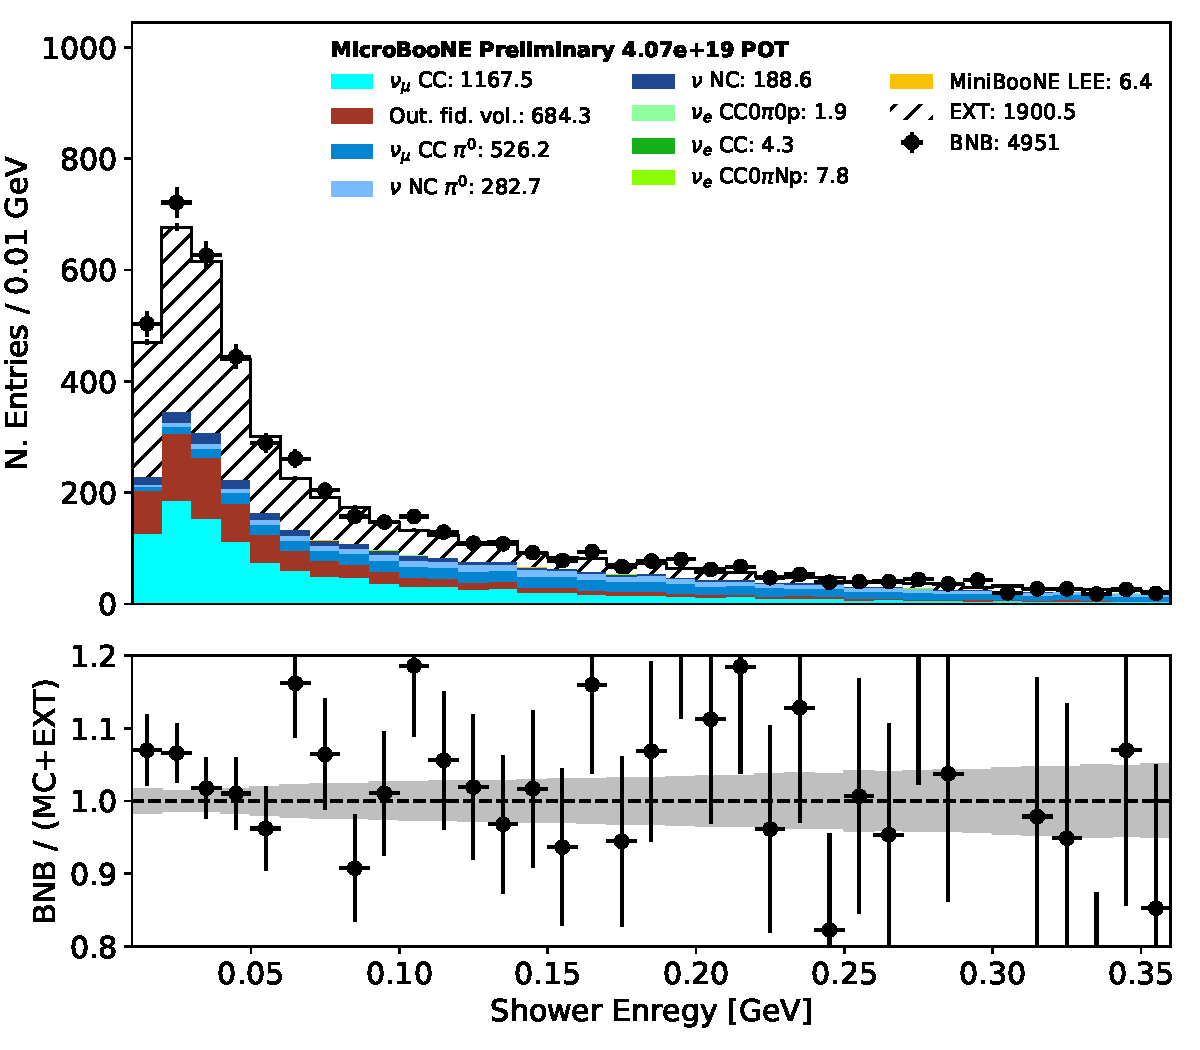
\includegraphics[width=1.00\textwidth]{nueselection/shr_energy_tot_cali_01132020_RUN1.pdf}
    \caption{\label{fig:nue:presel:shrenergy} }
    \end{subfigure}
\caption{\label{fig:nue:presel}Variables input to the common $\nu_e$ N$p$ and 0$p$ pre-selections.}
\end{center}
\end{figure}

\par The efficiencies of the 1$e$N$p$ and 1$e$0$p$ pre-selections are shown in figure~\ref{fig:nue:presel:eff}. Efficiencies are presented as a function of true neutrino energy~\ref{fig:nue:presel:eff:nu}, proton KE~\ref{fig:nue:presel:eff:proton}, and electron energy~\ref{fig:nue:presel:eff:elec}. Each plot shows in black the efficiency for the common pre-selection (before a proton requirement is or is not imposed) and is reported relative to all intrinsic $\nu_e$ events. In blue and red respectively are shown the efficiencies for the  1$e$N$p$ and 1$e$0$p$ selections respectively, relative to true N$p$ and 0$p$ events. Shaded histograms in red and blue show the stacked truth-level distributions for N$p$ and 0$p$ events for the variables being plotted.

\begin{figure}[H] 
\begin{center}
    \begin{subfigure}[b]{0.3\textwidth}
    \centering
    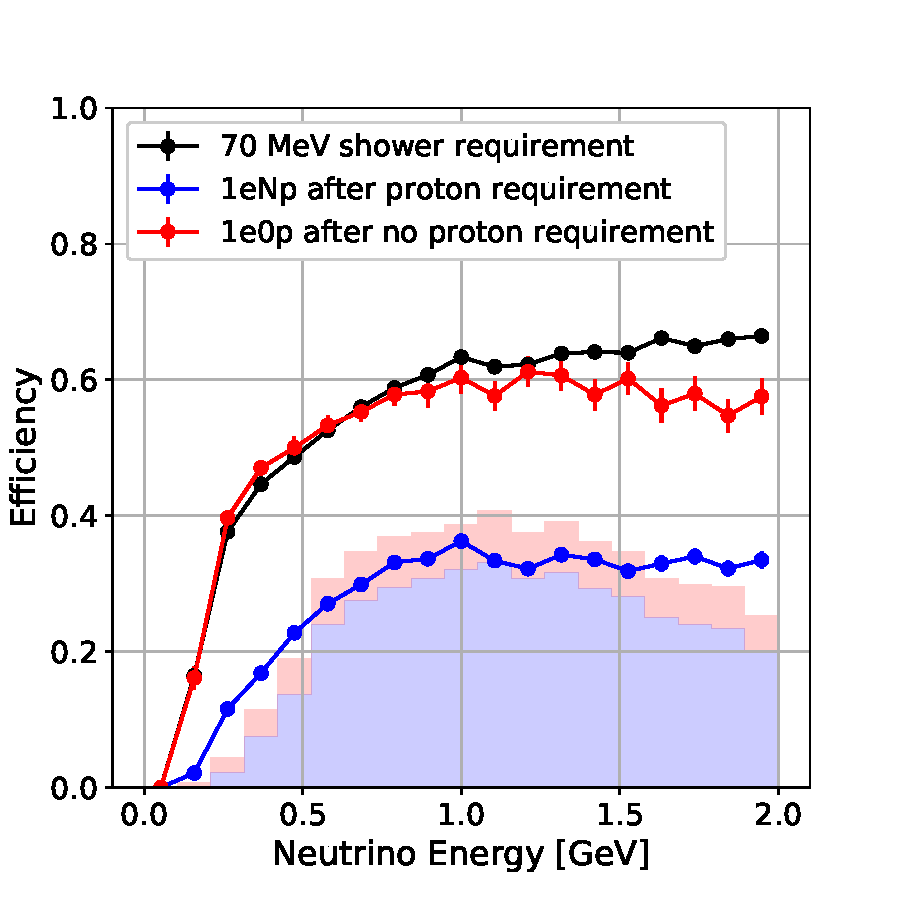
\includegraphics[width=1.00\textwidth]{nueselection/nu_RUN1.pdf}
    \caption{\label{fig:nue:presel:eff:nu} }
    \end{subfigure}
    \begin{subfigure}[b]{0.3\textwidth}
    \centering
    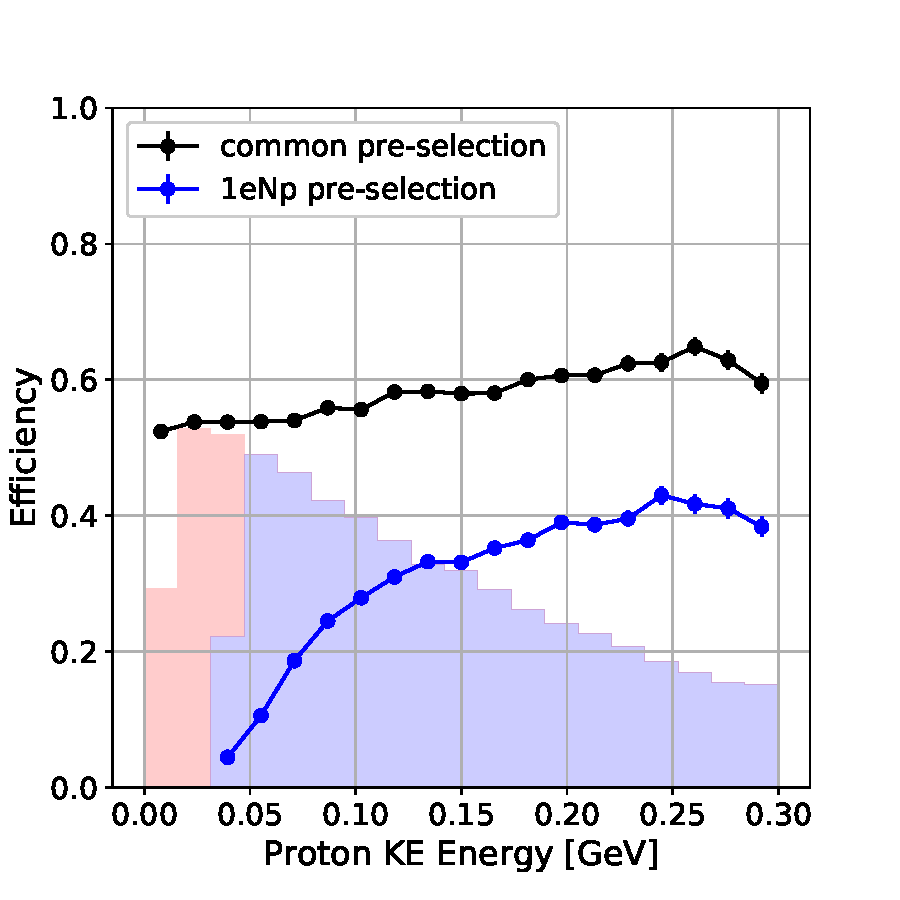
\includegraphics[width=1.00\textwidth]{nueselection/proton_RUN1.pdf}
    \caption{\label{fig:nue:presel:eff:proton} }
    \end{subfigure}
    \begin{subfigure}[b]{0.3\textwidth}
    \centering
    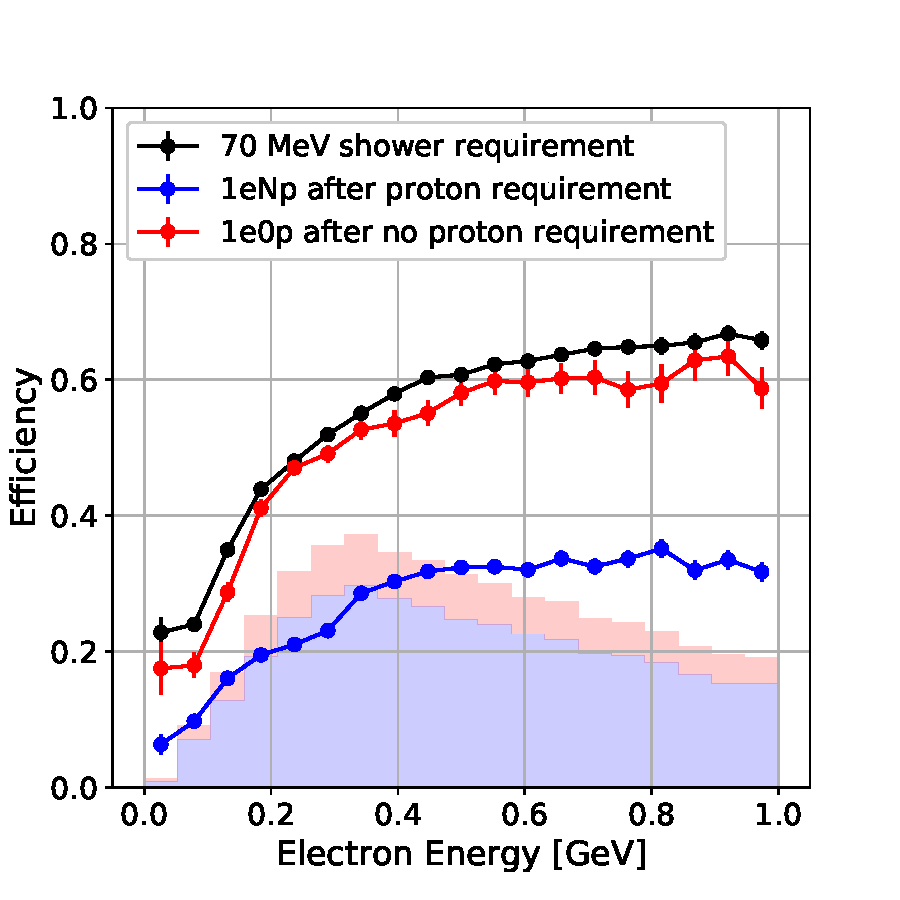
\includegraphics[width=1.00\textwidth]{nueselection/elec_RUN1.pdf}
    \caption{\label{fig:nue:presel:eff:elec} }
    \end{subfigure}
\caption{\label{fig:nue:presel:eff}}
\end{center}
\end{figure}

\subsection{Variable definitions}
\label{sec:nueselection:variables}
\par Variables used for the $\nu_e$ selections aim to isolate features in the neutrino interaction that are specific to events with final-state electrons. These features are split in several categories:

\begin{figure}[H]
\begin{center}
\includegraphics[width=0.6\textwidth]{nueselection/tools.png}
\caption{\label{fig:nue:variables}Categories of variables leveraged in the $\nu_e$ selections.}
\end{center}
\end{figure}

\par \noindent  \textbf{Slice variables}: these are variables associated to general features of the reconstructed neutrino interaction or event.

\begin{itemize}
    \item \emph{nslice}: number of neutrino slices identified by the SliceId (possible values are 0 and 1);
    \item \emph{reco\_nu\_vtx\_sce\_\{x,y,z\}}: Reconstructed space charged corrected neutrino interaction vertex in (x,y,z) coordinates.
    \item \emph{n\_showers\_contained}: number of showers with a starting point within the fiducial volume;
    \item \emph{n\_tracks\_contained}: number of tracks fully contained in the fiducial volume;
    \item \emph{contained\_fraction}: fraction of hits in PFParticles contained in the fiducial volume (according to definitions above) with respect to the total number of clustered hits in the slice;
    \item \emph{hits\_ratio}: ratio between hits from showers and total number of hits;
    \item \emph{CosmicIP}: closest distance between shower start and space points associated to tracks flagged as cosmics.
    \item \emph{crtveto}: boolean variable checking whether the event passes the CRT veto or not
    \item \emph{\_closestNuCosmicDist}: minimum 3D distance of the reconstructed neutrino vertex from a CRT-tagged cosmic track
\end{itemize}

\par \noindent \textbf{Shower and Track variables}:

\begin{itemize}
    \item \emph{tksh\_distance}: distance between leading shower vertex and longest track vertex;
    \item \emph{tksh\_angle}: angle between leading shower vertex and longest track vertex;
    item \emph{merge\_bestdist}: Distance between shower start point and track start (or end) point for the track in the slice that best matches the direction of the shower. 
\end{itemize}

\par \noindent \textbf{Shower variables}:

\begin{itemize}
    \item \emph{shr\_energy\_tot\_cali}: sum of the energy of the calibrated showers (in GeV);
    \item \emph{shr\_tkfit\_2cm\_dedx\_\{U,V,Y\}}: dE/dx in the first 2 cm of the leading shower on plane (U,V,Y) with the track fitting;
    \item \emph{shr\_tkfit\_gap10\_dedx\_\{U,V,Y\}}: dE/dx in the [1,5] cm range of the leading shower on plane (U,V,Y) with the track fitting;
    \item \emph{shr\_score}: Pandora SVM track/shower score for the leading shower;
    \item \emph{shrmoliereavg}: average angle between the vector connecting the shower start to each shower space point and the shower direction vector
    \item \emph{subcluster}: number of subclusters (counted in all planes) for the leading shower.
    \item \emph{trkfit}: ratio of hits fitted in the track fit to the shower to all hits in the shower.
\end{itemize}

\par \noindent  \textbf{Track variables}:

\begin{itemize}
    \item \emph{trkpid}: proton-muon LLR particle identification 
\end{itemize}

\par \noindent  \textbf{2nd shower-based $\pi^0$ rejection variables}:

\begin{itemize}
    \item \emph{secondshower\_Y\_nhit}: number of hits in the collection plane of the largest cluster associated to the  recovered 2nd shower
    \item \emph{secondshower\_Y\_dot}: dot product between the vector connecting the vertex to the closest hit in cluster and the charge-weighted cluster direction w.r.t. closest hit in cluster
    \item \emph{anglediff\_Y}: 2D angle difference in the collection plane between the 2nd shower and the 1st shower cluster  (cluster direction defined as charge-weighted direction of cluster w.r.t. vertex)
    \item \emph{secondshower\_Y\_vtxdist}: 2D distance from vertex for the largest 2D cluster associated to the  recovered 2nd shower in the collection plane
\end{itemize}

\subsection{Inclusive Channel \textcolor{red}{Wouter}}
\label{sec:nueselection:inclusive}

\subsection{1$e$N$p$ Channel \textcolor{red}{David + Giuseppe}}
\label{sec:nueselection:1eNp}

The 1$e$N$p$ channel is the most sensitive to the MiniBooNE eLEE signal as it contains a large fraction of the signal events and allows for selection requirements based both on showers and tracks. 
Given the large cosmic background and that $\nu_e$ charge-current interactions are O(1\%) in the BNB, a high-purity selection is needed to achieve a sizeable signal sensitivity. 

We first define a set of minimal requirements ("preselection") to obtain a high statistics sample (dominated by cosmic and neutrino backgrounds) that is used to monitor the data-MC agreement of the selection variables. 
We then define two alternative selections, respectively based on a simple box-cut approach and on boosted decision trees (BDT); the BDT approach is clearly the most sensitive, while box-cuts provide a robust reference selection.

\subsubsection{Preselection}

At preselection stage we apply the minimum set of requirements so that all selection variabes can be defined, plus the containment and a minimum shower energy to reject Michel electrons:
\begin{itemize}
    \item nslice = 1
    \item n\_tracks\_contained $>$ 0
    \item n\_showers\_contained $>$ 0
    \item contained\_fraction $>$ 0.9
    \item shr\_energy\_tot\_cali $>$ 0.07
\end{itemize}

\par 
Topics to discuss: selection efficiency and purity, data-MC agreement of selection variables.

\begin{figure}[ht] 
\begin{center}
    \begin{subfigure}[b]{0.45\textwidth}
    \centering
    \includegraphics[width=1.00\textwidth]{1eNp/reco_e_01122020_RUN1.pdf}
    \caption{\label{fig:1eNp:prsel:RUN1} RUN 1}
    \end{subfigure}
    \begin{subfigure}[b]{0.45\textwidth}
    \centering
    \includegraphics[width=1.00\textwidth]{1eNp/reco_e_01122020_RUN3.pdf}
    \caption{\label{fig:1eNp:prsel:RUN1} RUN 3}
    \end{subfigure}
\caption{\label{fig:1eNp:prsel}pre-selection for 1$e$N$p$ channel}
\end{center}
\end{figure}

\subsubsection{Box-cuts}

In addition to the preselection requirements, cuts are applied to suppress specific backgrounds. Note however that, to the extent that some variables are effective against multiple backgrounds, the following description is a simplification.

First, we aim at rejecting cosmic-induced events by requiring large CosmicIP and a proton-like trkpid. The latter requirement in particular rejects more than 90\% of the cosmics that pass pre-selection.

Next, the goal is to suppress events from $\nu_\mu$ charged current interactions. We require shower hits to be the dominant in the slice, and imposing tight quality requirements on the shower object (shr\_score, shrmoliereavg, trkfit, subcluster).

At this stage, most of selected events contain neutrino-induced electromagnetic activity so that main background are events with $\pi^0$. They are rejected requiring only one shower in the event, a small distance between the track and shower start points, that the shower dEdx can be evaluated at least on the collection plane and it is not consistent with two or more MIPs in any plane (using two different dEdx definitions).

Finally, in order to avoid misreconstructed events, events where the track and shower are aligned are rejected.

For reference, the full list of cuts is:
\begin{itemize}
    \item CosmicIP $>$ 20.
    \item trkpid $<$ -0.02
    \item hits\_ratio $>$ 0.60
    \item shr\_score $<$ 0.275
    \item shrmoliereavg $>$ 2 and shrmoliereavg $<$ 9
    \item trkfit $<$ 0.45 or subcluster $>$ 6
    \item n\_showers\_contained = 1
    \item tksh\_distance $<$ 3.5
    \item shr\_tkfit\_2cm\_dedx\_Y $\in$ [0,4.0] and shr\_tkfit\_2cm\_dedx\_U $<$ 4.0 and shr\_tkfit\_2cm\_dedx\_V $<$ 4.0
    \item shr\_tkfit\_gap10\_dedx\_Y $\in$ [0,4.5] and shr\_tkfit\_gap10\_dedx\_U $<$ 4.5 and shr\_tkfit\_gap10\_dedx\_V $<$ 4.5
    \item secondshower\_Y\_nhit $\leq$ 8 or secondshower\_Y\_dot $\leq$ 0.8 or anglediff\_Y $\leq$ 40 or secondshower\_Y\_vtxdist $\geq$ 100
    \item tksh\_angle $>$ -0.9 and tksh\_angle $<$ 0.7
\end{itemize}

\par 
Topics to discuss: selection efficiency and purity, expected number of events in open data and in full sample.

\begin{figure}[ht]
\begin{center}
\includegraphics[width=0.45\textwidth]{1eNp/reco_e_01122020_RUN1_box.pdf}
\caption{\label{fig:1eNp:box:RUN1}Box-cuts for 1$e$N$p$ channel.}
\end{center}
\end{figure}

\subsubsection{BDT}

Two BDTs are trained separately to reject backgrounds with and without $\pi^0$ in the final state. The same set of training variables is used in the two BDTs, corresponding to the list of variables used in the box-cut selection. 

Both in the training and in the analysis, events are required to pass the preselection requirements plus a loose set of cuts intended to avoid considering events where one or more variables is clearly inconsistent with $\nu_e$ events. The list of cuts is:
\begin{itemize}
    \item CosmicIP $>$ 20.
    \item trkpid $<$ 0.1
    \item hits\_ratio $>$ 0.5
    \item shr\_score $<$ 0.30
    \item n\_showers\_contained = 1
    \item tksh\_distance $<$ 6.0
    \item shr\_tkfit\_2cm\_dedx\_Y $<$ 4.0
    \item tksh\_angle $>$ -0.9
\end{itemize}

Indeed the BDT is able to figure out during training which variables are most important for each background: shower quality variables (e.g. shr\_score, trkfit, subcluster) have higher ranking for the non-$\pi^0$ BDT, while variables such as tksh\_distance and the shower dEdx show higher importance for the $\pi^0$-BDT. It is interesting to note that the most discriminating variable is in both cases shrmoliereavg which may be useful to discriminate both muons in $\nu_\mu$ events (low values) and merged showers in $\pi^0$ events (large values).

\begin{table}[h!]
\centering
 \begin{tabular}{c | c c | c c} 
 \hline
& \multicolumn{2}{c |}{$\pi^0$ BDT} & \multicolumn{2}{c}{non-$\pi^0$ BDT} \\
 \hline
Rank & Variable & Importance & Variable & Importance \\
 \hline
1 & shrmoliereavg & 5813 & shrmoliereavg & 6436 \\ 
2 & tksh\_distance & 2834 & trkfit & 3309 \\
3 & trkpid & 2306 & shr\_tkfit\_2cm\_dedx\_ALL & 1980 \\
4 & shr\_tkfit\_2cm\_dedx\_ALL & 2225 & subcluster & 1908 \\
5 & secondshower\_Y\_vtxdist & 1891 & shr\_score & 1851 \\
6 & shr\_tkfit\_gap10\_dedx\_ALL & 1702 & trkpid & 1778 \\
7 & shr\_score & 1572 & secondshower\_Y\_vtxdist & 1405 \\
8 & trkshrhitdist2 & 1286 & shr\_tkfit\_gap10\_dedx\_ALL & 1293 \\
9 & trkfit & 1101 & tksh\_distance & 981 \\
10 & secondshower\_Y\_nhit & 1015 & secondshower\_Y\_nhit & 976 \\
11 & hits\_ratio & 949 & anglediff\_Y & 914 \\
12 & tksh\_angle & 929 & trkshrhitdist2 & 903 \\
13 & anglediff\_Y & 831 & tksh\_angle & 881 \\
14 & subcluster & 699  & hits\_ratio & 657 \\
15 & secondshower\_Y\_dot & 680 & secondshower\_Y\_dot & 592 \\
 \hline
\end{tabular}
\caption{Ranking of BDT variables based on their importance in terms of "total gain". dEdx variables are combined for different planes (note the "ALL" suffix).}
\label{tab:bdtimp}
\end{table}

We then cut separately on the output of the two BDTs, requiring pi0\_score $>$ 0.995 and nonpi0\_score $>$ 0.9984.

\par 
Topics to discuss: selection efficiency and purity, expected number of events in open data and in full sample.

\begin{figure}[H] 
\begin{center}
    \begin{subfigure}[b]{0.45\textwidth}
    \centering
    \includegraphics[width=1.00\textwidth]{1eNp/nonpi0_score_01122020_RUN1.pdf}
    \caption{\label{fig:1eNp:bdt:nonpi0:all}}
    \end{subfigure}
    \begin{subfigure}[b]{0.45\textwidth}
    \centering
    \includegraphics[width=1.00\textwidth]{1eNp/nonpi0_score_01122020_zoom_RUN1.pdf}
    \caption{\label{fig:1eNp:bdt:nonpi0:zoom}}
    \end{subfigure}
\caption{\label{ffig:1eNp:bdt:nonpi0}BDT resposne for non-$\pi^0$ BDT after 1$e$N$p$ pre-selection}
\end{center}
\end{figure}


\begin{figure}[H] 
\begin{center}
    \begin{subfigure}[b]{0.45\textwidth}
    \centering
    \includegraphics[width=1.00\textwidth]{1eNp/pi0_score_01122020_RUN1.pdf}
    \caption{\label{fig:1eNp:bdt:pi0:all}}
    \end{subfigure}
    \begin{subfigure}[b]{0.45\textwidth}
    \centering
    \includegraphics[width=1.00\textwidth]{1eNp/pi0_score_01122020_zoom_RUN1.pdf}
    \caption{\label{fig:1eNp:bdt:pi0:zoom}}
    \end{subfigure}
\caption{\label{ffig:1eNp:bdt:pi0}BDT resposne for $\pi^0$ BDT after 1$e$N$p$ pre-selection}
\end{center}
\end{figure}

\begin{figure}[H]
\begin{center}
\includegraphics[width=0.45\textwidth]{1eNp/reco_e_01122020_bdt_RUN1.pdf}
\caption{\label{fig:1eNp:box:RUN1}BDT-based selection for 1$e$N$p$ with cuts at 0.995 and 0.9984 for the $\pi^0$ and non-$\pi^0$ variables respectively.}
\end{center}
\end{figure}


\subsection{1$e$0$p$ Channel \textcolor{red}{Sophie, Ivan}}
\label{sec:nueselection:1e0p}
Selection motivation:

\subsubsection{Tools Unique to 0p Selection}
Shower-Track merging to recover signal orthogonal to Np selection.

\subsubsection{Pre-selection}
Data-MC comparisons:

\subsubsection{Box cut selection}

\subsubsection{BDT}

\clearpage
\section{$\nu_{\mu}$ Selection \textcolor{red}{Ryan, Wouter}}
\label{sec:NuMUCCsel}

\par This chapter presents the two $\nu_{\mu}$ selections of the analysis; both are inclusive selections, but with different distributions. The first selection (sec \ref{ssec:NuMUCCsel:INC}) provides a pure, high-statistics sample of $\nu_{\mu}$s and the second selection (sec \ref{ssec:NuMUCCsel:constr}) is optimized to be used as a constraining tool in the $\nu_e$ analysis \textcolor{blue}{with a particular emphasis on reconstructing low-energy neutrino interactions}. 
\textcolor{blue}{The inclusive selection of Sec.~\ref{ssec:NuMUCCsel:INC} is particularly well suited as a filter for multiple exclusive channel measurements, which, while not currently performed and included in this analysis, may provide helpful and necessary validations and constraints on neutrino interaction modeling as the analysis matures in the coming months.}

\subsection{Variable Definitions}
\label{ssec:NuMUCCsel:sel:vars}

\par Table~\ref{tab:numuvariableSummary} contains a concise list of variables used in the $\nu_{\mu}$ selections. The variables are organized into \textit{slice} and \textit{track}-level descriptors, used for preselection and muon-candidate selection respectively. There is some redundancy between this list and the list in sec \ref{sec:nueselection:variables}, but this list below should serve as a quick reference to a reader of this chapter.

\begin{table}[ht]
\caption{\label{tab:numuvariableSummary} Summary of the definition for the variables used in the $\nu_{\mu}$ selections.}
\centering
\begin{tabular}{ m{0.08\textwidth} | m{0.25\textwidth} | m{0.55\textwidth}  }
Category & Variable Name & Description  \\
\hline

\multicolumn{1}{l|}{} & \emph{nslice} &  Number of neutrino slices identified by the \emph{SliceID}. Values are  0 or 1.\\  \cline{2-3}
\multicolumn{1}{l|}{} & \emph{slpdg} &  PDG code of the event as assigned by Pandora, 12 if the object with the most hits over all planes is shower-like, 14 if track-like.\\  \cline{2-3}
\multicolumn{1}{l|}{} & \emph{all\_\{start,end\}\_contained} &  The start/end points of all PFParticles are volume defined with borders: \SI{5}{\cm} in $x$ and \SI{6}{\cm} $y$ and \SI{10}{\cm} $z$.\\  \cline{2-3}
\multicolumn{1}{l|}{} & \emph{slpdg} &  PDG code of the event as assigned by Pandora, 12 if the object with the most hits over all planes is shower-like, 14 if track-like.\\  \cline{2-3}
\multicolumn{1}{l|}{} & \emph{n\_tracks\_contained} &  number of tracks fully contained in the fiducial volume.\\  \cline{2-3}
\multicolumn{1}{l|}{} & \emph{reco\_nu\_vtx\_sce\_\{x,y,z\}} & Reconstructed neutrino interaction vertex in (x,y,z) coordinates. The space charged correction is applied.  \\  \cline{2-3}
\parbox[t]{2mm}{\multirow{4}{*}{\rotatebox[origin=c]{90}{Slice}}} & \emph{hits\_ratio} & Ratio between hits from showers and total number of hits in the slice. \\  \cline{2-3}
\multicolumn{1}{l|}{} & \emph{CosmicIP} & Closest distance between shower start and space points associated to tracks flagged as cosmics. \\  \cline{2-3}
\multicolumn{1}{l|}{} & \emph{crtveto} & Boolean variable checking if the event passes the CRT veto. \\  \cline{2-3}
\multicolumn{1}{l|}{} & \emph{\_closestNuCosmicDist} &  3D distance between the reconstructed neutrino vertex and the closest CRT-tagged cosmic track. \\  \cline{2-3}
\hline


\multicolumn{1}{l|}{} & \emph{trk\_sce\_\{start,end\}\_\{x,y,z\}} &  Reconstructed, spacecharge-corrected start/end-points for the tracks.\\  \cline{2-3}
\multicolumn{1}{l|}{} & \emph{trk\_llr\_pid\_score} &  The log likelihood ratio particle identification score (see sec. \ref{subsec:loglikelihoodpid}). This variable has strong muon-proton discriminating power (see fig. \ref{fig:numu_topo_pid}).\\  \cline{2-3}
\multicolumn{1}{l|}{} & \emph{trk\_score} & A machine-learned quantity that describes how `track-like' the reconstructed object is (possible values between 0 and 1). \\  \cline{2-3}
\parbox[t]{2mm}{\multirow{4}{*}{\rotatebox[origin=c]{90}{Track}}} & \emph{trk\_len} & he length of the reconstructed track (in cm). \\  \cline{2-3}
\multicolumn{1}{l|}{} & \emph{trk\_distance} & The distance from the start-point of the reconstructed track to the reconstructed neutrino vertex (in cm). \\  \cline{2-3}
\multicolumn{1}{l|}{} & \emph{pfp\_generation} & The generation of the PFParticle according to Pandora, i.e. how many parents the object on interest has in the slice.\\  \cline{2-3}
\hline

\end{tabular}
\label{tab:numuvariableSummary}
\end{table}

\begin{comment}

\par \noindent \textbf{Slice variables}: These variables generally describe the reconstructed neutrino interaction, i.e. the confluence of data gathered from all the PFParticles in the slice.
\begin{itemize}
    \item \emph{nslice}: number of neutrino slices identified by the SliceID (possible values are 0 or 1).
    \item \emph{n\_tracks\_contained}: number of tracks fully contained in the fiducial volume.
    \item \emph{reco\_nu\_vtx\_sce\_\{x,y,z\}}: Reconstructed, spacecharge-corrected neutrino interaction vertices in (x,y,z) coordinates (see fig. \ref{fig:numu_vtx}.
    \item \emph{topological\_score}: A machine-learned quantity that reflects the complexity and directionality of observable slice quantities. This variable has strong discriminating power between signal and cosmic-background (see \ref{fig:numu_topo_pid} (possible values are between 0 and 1).
    \item \emph{CRT Veto and Distance Tagger}: Tools provided by the cosmic ray tagger (see sec. \ref{sec:sliceID:CRT}).
\end{itemize}

\par \noindent \textbf{Track variables}: These variables specifically describe the reconstructed PFParticles; in interest to this selection are reconstructed track-like objects. 
\begin{itemize}
    \item \emph{trk\_sce\_\{start,end\}\_\{x,y,z\}}: Reconstructed, spacecharge-corrected start/end-points for the tracks.
    \item \emph{trk\_llr\_pid\_score}: The log likelihood ratio particle identification score (see sec. \ref{subsec:loglikelihoodpid}). This variable has strong muon-proton discriminating power (see fig. \ref{fig:numu_topo_pid}).
    \item \emph{trk\_score}: A machine-learned quantity that describes how `track-like' the reconstructed object is (possible values between 0 and 1).
    \item \emph{trk\_len}: The length of the reconstructed track (in cm).
    \item \emph{trk\_distance}: The distance from the start-point of the reconstructed track to the reconstructed neutrino vertex (in cm).
    \item \emph{pfp\_generation}: The generation of the PFParticle according to Pandora, i.e. the neutrino has generation 1, its direct daughters generation 2 and further decay products have generation 3.
\end{itemize}
\end{comment}

\begin{comment}
\subsubsection{Backgrounds}
\label{sssec:NuMUCCsel:sel:bkgrnds}

\par Coming soon...

\subsubsection{Fiducial Volume and Spacecharge-Corrected Spacepoints}
\label{sssec:NuMUCCsel:sel:FVandSCE}

\par Coming soon...
\end{comment}



\subsection{Inclusive Selection}
\label{ssec:NuMUCCsel:INC}
The $\nu_\mu$ CC Inclusive selection is an update from the selection that is currently be used as a filter and described in an internal note~\cite{bib:numuccfilter}. This selection aims to be as similar as possible to the $\nu_e$ CC Inclusive selection described in \cref{sec:nueselection:inclusive}, with the ultimate goal to perform a $\nu_\mu$ constrained BNB electron neutrino measurement. 

\paragraph{$\nu_\mu$ CC inclusive signal definition}
\begin{itemize}
    \item One final state muon with a kinetic energy above \SI{20}{\MeV}.
    \item True neutrino vertex inside a fiducial volume defined with borders: \SI{10}{\cm} in $x$ and $y$ and $[ \SI{20}{\cm}, \SI{50}{\cm}]$ in $z$.
\end{itemize}
The cut on the true energy corresponds to a track length of \SI{\approx 2.5}{\cm}.

\paragraph{Event selection}
Before identifying the muon, some event level cuts are applied:

\begin{itemize}
    \item \textit{slpdg==14}
    \item \textit{CosmicIP} $>$ \SI{20}{\cm}
    \item \textit{topological\_score $>$ 0.1}
    \item \textit{all\_start\_contained}
    \item reco\_fid\_vol \& CosmicIP>20 \& slpdg==14 \& all\_start\_contained
\end{itemize} 

The next step is to identify a muon track.
\paragraph{Muon candidate identification} 
\begin{itemize}
    \item \textit{trk\_score $>$ 0.8}
    \item \textit{trk\_len} $>$ \SI{10}{\cm}
    \item \textit{trk\_llr\_pid\_score $>$ 0.2}
    \item \textit{pfp\_generation==2}
    \item \textit{trk\_distance} $<$ \SI{4}{\cm}
\end{itemize}
At this point, the amount of muon candidate tracks in signal events is:
\begin{itemize}
    \item 0 (10\%), the event gets rejected.
    \item 1 (70\%), the event gets selected.
    \item 2 (18\%) or $>2$ (2\%), the particle with the highest \textit{trk\_llr\_pid\_score} is picked as muon and the event is selected.
\end{itemize}

The cut on the reconstructed length corresponds to a muon kinetic energy of \SI{\approx 47}{\MeV} kinetic energy or a muon momentum of \SI{0.11}{GeV/c}. Therefore, this selection aim to have a lower neutrino energy threshold of \SI{\approx 153}{\MeV}. Therefore, efficiency plots will be shown in a range from \SIrange{0.15}{1.65}{\GeV} in this section.

\begin{figure}
    \centering
    \includegraphics[width=\textwidth]{NuMuCCsel/Images/run1/numu_pret_run1.pdf}
    \caption{Topological score and track PID likelihood distributions after all other cuts are applied in the $\nu_\mu$ CC inclusive selection.}
    \label{fig:numu:topo_pid}
\end{figure}

The distribution of the topological score and the track muon likelihood after applying all cuts except these two is given in \cref{fig:numu:topo_pid}.

\paragraph{Event selection performance}

\begin{figure}[H]
    \centering
    \includegraphics[width=0.65\textwidth]{NuMuCCsel/Images/run1/numu_efficiency_run1.pdf}
    \caption{Efficiency of the $\nu_\mu$ CC inclusive selection for different interaction categories (left) and final states (right) in function of the true neutrino energy. }
    \label{fig:numu:eff_r1}
\end{figure}

\cref{fig:numu:eff_r1} shows the efficiency in function of the true neutrino energy, integrated over all energies for all singal event categories, the efficiency is 51.1\%. It can be seen that the selection is truly inclusive in both interaction type and final states. non-zero efficiencies are reached from \SI{150}{\MeV} and the efficiency flattens out at \SI{\approx 700}{\MeV}. The overall purity of the selection is 65.9\% with the in-time cosmic activity as dominant background. In 94.7\% of the events, the track identified as muon is backtracked to the muon correctly. Most mis-identification cases correspond to charged pions (3.6\%).

Because this selection contains both contained and uncontained events, multiple coulomb scattering is used to measure the muon momentum. \cref{fig:numu:mcs,fig:numu:angles,fig:numu:vtx} show the 


\begin{figure}[H]
    \centering
    \includegraphics[width=0.495\textwidth]{NuMuCCsel/Images/run1/numu_mcsmom_run1.pdf} \hfill
    \includegraphics[width=0.495\textwidth]{NuMuCCsel/Images/run1/numu_vtxntrack_cat_run1.pdf}
    \caption{Caption}
    \label{fig:numu:mcs}
\end{figure}

\begin{figure}[H]
    \centering
    \includegraphics[height=6.5cm]{NuMuCCsel/Images/run1/numu_theta_run1.pdf} \hspace{2mm}
    \includegraphics[height=6.5cm]{NuMuCCsel/Images/run1/numu_phi_run1.pdf}
    \caption{Caption}
    \label{fig:numu:angles}
\end{figure}

\begin{figure}[H]
    \centering
    \includegraphics[width=\textwidth]{NuMuCCsel/Images/run1/numu_recovtx_run1.pdf}
    \caption{Caption}
    \label{fig:numu:vtx}
\end{figure}

\subsubsection{Run3}
\label{sssec:NuMUCCsel:INC:Run3}

\begin{figure}[H]
    \centering
    \includegraphics[width=0.85\textwidth]{NuMuCCsel/Images/run3/numu_efficiency_run3.pdf}
    \caption{Caption}
    \label{fig:numu_eff_r3}
\end{figure}


\begin{figure}[H]
    \centering
    \includegraphics[height=6.5cm]{NuMuCCsel/Images/run3/numu_rangemom_run3.pdf} \hspace{2mm}
    \includegraphics[height=6.5cm]{NuMuCCsel/Images/run3/numu_caloe_run3.pdf}
    \caption{Caption}
    \label{fig:numu_energy}
\end{figure}

\begin{figure}[H]
    \centering
    \includegraphics[height=6.5cm]{NuMuCCsel/Images/run3/numu_theta_run3.pdf} \hspace{2mm}
    \includegraphics[height=6.5cm]{NuMuCCsel/Images/run3/numu_phi_run3.pdf}
    \caption{Caption}
    \label{fig:numu_angles}
\end{figure}

\subsection{$\nu_{\mu}$ Constraint Selection \textcolor{red}{Ryan}}
\label{ssec:NuMUCCsel:constr}
\par The purpose of this $\nu_{\mu}$ side-band is to constrain the systematic uncertainties in the $\nu_{e}$ analysis. This is able to be done because the $\nu_{\mu}$s and $\nu_{e}$s of the BNB are subject to common, correlated uncertainties for flux and cross-section modelling uncertainties. The $\nu_{e}$ selection is subject to higher uncertainties due to its low statistics. The $\nu_{\mu}$ channel benefits from two orders-of-magnitude larger absolute flux (Docdb 1031) therefore providing high-statistics samples which can be exploited to constrain the uncertainties on the $\nu_{e}$ predicted event rate. For more information regarding the philosophy and goals of this constraint see sec \ref{ssec:goalsofnumusel}.

\par This selection prioritizes higher efficiencies and purities in the low-energy region that is the interest to the LEE analysis. Unfortunately, the flux and cross-section predictions for $\nu_{e}$ are most uncertain in the few-hundreds MeV energy region. Fortunately, the absolute $\nu_{\mu}$ flux and the cross-species flux correlation is greatest below 1 GeV (see figs \ref{fig:numuconstraint:flux}, \ref{fig:numuconstraint}).
\begin{comment}
\begin{figure}
    \centering
    \includegraphics[height=6.5cm]{NuMuCCsel/Images/Ryan/absoluteFlux_uBooNE.png} \hspace{2mm}
    \caption{The absolute neutrino flux prediction through the MicroBooNE detector as calculated by the beam simulation. Shown is the flux for $\nu_{\mu}$, $\overline{\nu_{\mu}}$, $\nu_{e}$, and $\overline{\nu_{e}}$ averaged through the TPC volume with dimensions 2.56m by 2.33m by10.37m. DocDb 1031}
    \label{fig:bnb_absoluteflux}
\end{figure}
\end{comment}
\subsubsection{Signal Definition}
\label{sssec:NuMUCCsel:constr:signaldef}
\par A $\nu_{\mu}$ event is identified by the presence of one muon candidate originating from inside the fiducial volume of the detector. Additional tracks and showers may accompany the muon candidate; these assist in reconstruction but are not necessary in the inclusive selection. Future studies of the $\nu_{\mu}$ side-band may require the presence of proton candidates to further constrain interaction models.

\subsubsection{Event Preselection}
\label{sssec:NuMUCCsel:constr:preselec}

\par The selection of $\nu_{\mu}$ events is built from the groundwork of the SliceID tool (see sec. \ref{sec:sliceID:SliceID}) and a combination of cuts on event-level and track-level observable values. The cuts in this section are primarily designed to eliminate cosmic and dirt backgrounds and select slices that are $\nu_{\mu}$-like. The methodology of this selection is similar to the selections in sec \ref{sec:nueselection} where first, the common SliceID filter is applied; next, event-level cuts are applied to select $\nu_{\mu}$-like events; finally, track-level cuts are applied to screen for muon-like candidates. The muon-candidate selection is described in sec \ref{sssec:NuMUCCsel:constr:muonsel}.

\par The requirement that the reconstructed vertex be contained inside the fiducial volume and that the slice have a sufficiently high topological score favor $\nu_{\mu}$ CC events and disfavor activity that is cosmogenic or dirt-like. Those cuts, specifically, are:

\begin{itemize}
    \item \emph{nslice} = 1.
    \item \emph{n\_tracks\_contained} $>$= 1.
    \item \emph{reco\_nu\_vtx\_sce\_x} $\in$ [5,251] cm.
    \item \emph{reco\_nu\_vtx\_sce\_y} $\in$ [-110,110] cm.
    \item \emph{reco\_nu\_vtx\_sce\_z} $\in$ [20,986] cm.
    \item \emph{topological\_score} $>$ 0.06.
    \item \emph{reco\_nu\_vtx\_sce\_z} $\not\in$ [675,775] cm.
\end{itemize}

\par \noindent This selection defines a unique fiducial volume compared to other selections in this analysis. See sec \ref{sssec:NuMUCCsel:constr:FV} for discussion of the determination of this boundary. The final cut on the $z$ coordinate is to ensure that it is not in the region of `dead wires' in the MicroBooNE detector, this is common practice within this analysis and the larger collaboration.

\par \noindent Run 3 has the additional power to leverage the CRT system to further limit cosmic contamination in the signal. Given that this selection targets contained events, the fact that $\nu_{\mu}$ interactions can lead to hits in the CRT does not hamper the analysis' performance.

\textbf{Run 3 only:}
\begin{itemize}
    \item \emph{CRT Veto} != 1 or \emph{crthitpe} $<$ 100
    \item \emph{closestNuCosmicDist} $>$ 5 cm
\end{itemize}

\subsubsection{Muon Selection}
\label{sssec:NuMUCCsel:constr:muonsel}

\par After the event-level cuts are applied, the tracks in the slice are further analyzed to identify muon candidates. At least one reconstructed track in the event must satisfy all these criteria for the event to pass the selection. If more than one tracks pass this requirement, the longest is taken as the muon candidate. Of the muon candidates that pass this selection, $\approx 94\%$ are, in simulation, correctly tagged muons from $\nu_{\mu}$ CC interactions.

\begin{itemize}
    \item \emph{trk\_sce\_start\_x} $\in$ [5,251] cm.
    \item \emph{trk\_sce\_start\_y} $\in$ [-110,110] cm.
    \item \emph{trk\_sce\_start\_z} $\in$ [20,986] cm.
    \item \emph{trk\_sce\_end\_x} $\in$ [5,251] cm.
    \item \emph{trk\_sce\_end\_y} $\in$ [-110,110] cm.
    \item \emph{trk\_sce\_end\_z} $\in$ [20,986] cm.
    \item \emph{trk\_llr\_pid\_score} $>$ 0.2.
    \item \emph{trk\_trk\_score} $>$ 0.8.
    \item \emph{trk\_trk\_length} $>$ 10 cm.
    \item \emph{trk\_trk\_distance} $<$ 4 cm.
    \item \emph{pfp\_generation} = 2.
\end{itemize}

\par \noindent The cuts made on the start and end points of the reconstructed tracks require that the track is fully contained inside the fiducial volume of the detector. This containment cut further reduces the primary background for this selection are is cosmic muons, originating from outside the detector. The containment requirement also motivates the use of range-based momentum calculations on all the muon candidates. Range-based momentum has been shown to have a high resolution. \emph{Consistency between range-based and the independently calculated MCS-based momentum will be used in a future iteration of this analysis as an additional handle to increase purity (see figs \ref{fig:numusel:momres} and \ref{fig:NuMUCCsel:ryan:PQuality})}. The containment condition rejects many higher-energy $\nu_{\mu}$ events that might leave the detector, but it has a high efficiency in the lower energies.

\par The cut on the track distance requires that the reconstructed track be sufficiently close to the interaction vertex, this removes many in-time cosmic muons that are reconstructed as part of the event.

\par The cut on the log likelihood ratio pid score is to separate the muons from the protons among the PFParticle tracks in the passing slices. The track length cut further separates the muons from the protons which tend to have shorter track lengths. 

\par The track score cut ensures that the selected tracks are particularly track-like and this removes many \textcolor{red}{particularly high energy (unclear why this is the case)}, track-like showers from the selection. Finally the PFParticle generation cut ensures that Pandora recognizes that the track is produced directly at the neutrino interaction vertex, and not as a secondary particle (i.e. in a $\pi \rightarrow \mu$ decay or re-interaction). 

\begin{figure}
    \centering
    \includegraphics[height=6.5cm]{NuMuCCsel/Images/Ryan/containedMomentumRes.png} \hspace{2mm}
    \includegraphics[height=6.5cm]{NuMuCCsel/Images/Ryan/muoncandidate_pquality.jpg} \hspace{2mm}
    \caption{The performance of range-based $\mu$ momentum calculation for contained tracks.}
    \label{fig:numusel:momres}
\end{figure}

\begin{figure}[ht] 
\begin{center}
    \begin{subfigure}[b]{0.45\textwidth}
    \centering
    \includegraphics[width=1.00\textwidth]{NuMuCCsel/Images/Ryan/Run1_recoErange_FullSel.jpg}
    \caption{\label{fig:NuMUCCsel:ryan:noPQuality} After full selection.}
    \end{subfigure}
    \begin{subfigure}[b]{0.45\textwidth}
    \centering
    \includegraphics[width=1.00\textwidth]{NuMuCCsel/Images/Ryan/Run3_costheta_withCRT.jpg}
    \caption{\label{fig:NuMUCCsel:ryan:withPQuality} After full selection and momentum quality.}
    \end{subfigure}
\caption{The distribution of range-based energy calculations for each passing slice. Fig \ref{fig:NuMUCCsel:ryan:withPQuality} shows the distribution after a quality cut, keeping events that fall within 0.5 of the peak in the right plot of fig \ref{fig:numusel:momres}.}
\label{fig:NuMUCCsel:ryan:PQuality}
\end{center}
\end{figure}


\subsubsection{Determination of Fiducial Volume}
\label{sssec:NuMUCCsel:constr:FV}

\par This selection leverages the availability of a fully calibrated E-field map to perform space-charge corrections on the start and end-points of reconstructed tracks. This allows to impose a tight fiducial volume which maximizes the selection efficiency without impacting reconstruction performance. The fiducial volume is defined to be: 

\begin{itemize}
    \item x $\in$ [5,251]
    \item y $\in$ [-110,110]
    \item z $\in$ [20,986]
\end{itemize}

\begin{comment}
\par The fiducial volume in this section differs slightly from other fiducial volumes, even in this analysis. Because the purpose of this selection is to leverage the high-statistics of the $\nu_{\mu}$ composition of the BNB, the fiducial volume is taken to be as large as possible while retaining high purity and efficiency at low-energies.

\par With the exception of the downstream fiducial volume face, all the fiducial volume boundaries are chosen in order to retain as many signal events as possible. The SCE-correction procedure is quite effective and can recover the true value give or take a few centimeters, with slightly less resolution near the boundaries. The resolution is shown in fig \ref{fig:NuMUCCsel:ryan:sceres_y} for the x-direction; the performance is similar in the x, y, and z directions. See fig \ref{fig:NuMUCCsel:ryan:FVhighy} for an example of signal purity near a boundary using the spacecharge-corrected coordinates. Together, the spacecharge boundary that was found to maintain the highest purity is defined by


\begin{figure}
    \centering
    \includegraphics[height=6.5cm]{NuMuCCsel/Images/Ryan/sceresolution_y.jpg} \hspace{2mm}
    \caption{Resolution of the spacecharge-corrected vertex positions. The spacehcarge-corrected y-coordinates are being compared to the truth values without spacecharge distortion. }
    \label{fig:NuMUCCsel:ryan:sceres_y}
\end{figure}

\begin{figure}[ht] 
\begin{center}
    \begin{subfigure}[b]{0.45\textwidth}
    \centering
    \includegraphics[width=1.00\textwidth]{NuMuCCsel/Images/Ryan/Run3_MCData_highy.jpg}
    \caption{\label{fig:NuMUCCsel:ryan:FVhighyMC} Data-MC distribution near top of detector.}
    \end{subfigure}
    \begin{subfigure}[b]{0.45\textwidth}
    \centering
    \includegraphics[width=1.00\textwidth]{NuMuCCsel/Images/Ryan/SignalPurity_highy.png}
    \caption{\label{fig:NuMUCCsel:ryan:FVhighyPur} Signal Purity}
    \end{subfigure}
\caption{Example of signal composition near boundary.}
\label{fig:NuMUCCsel:ryan:FVhighy}
\end{center}
\end{figure}
\end{comment}

\subsubsection{Performance}
\label{sssec:NuMUCCsel:constr:performance}

\par This selection has been evaluated on the Run1 and the Run3 open datasets processed for this analysis. The advantage of the Run 1 data-set is higher statistics ($4E19$ POT in Run1 and $0.9E19$ POT in Run3). Run 3 allows to use the CRT system for extra background rejection. Distributions shown in this section will be of variables pertaining to the muon candidate for each event that passes the selection; Run1 data will be preferentially shown due to the higher statistics. The power of the Run3 CRT system will be demonstrated at the end of this section.

\par Run 3 data includes information from the CRT system which was unavailable for the first MicroBooNE run. See fig \ref{fig:NuMUCCsel:ryan:Run3CRTcomp} for an example of the impact of the CRT. The CRT veto will eliminate more than 70$\%$ of the cosmics while suffering only roughly 15$\%$ loss in signal.

\par The overall efficiency of this selection is \textcolor{pink}{finish remaking these plots with newest data} ???$\%$ and overall purity is ???$\%$. The priority of the selection was to maximize purity and efficiency in the low-energy region (see fig ???). The effectiveness of this selection can not by explained by distributions, efficiencies, and purities alone; it relies on the constraining power. See sec \ref{ssec:finalSensitivityCalc} for a technical discussion of the incorporation of this selection into the final analysis sensitivity.

\begin{figure}[H] 
\begin{center}
    \begin{subfigure}[b]{0.3\textwidth}
    \centering
    \includegraphics[width=1.00\textwidth]{NuMuCCsel/Images/Ryan/Run1_trklen_justSlice.jpg}
    \caption{\label{fig:NuMUCCsel:ryan:trklenSliceID} after SliceID}
    \end{subfigure}
    \begin{subfigure}[b]{0.3\textwidth}
    \centering
    \includegraphics[width=1.00\textwidth]{NuMuCCsel/Images/Ryan/Run1_trklen_justEvtsel.jpg}
    \caption{\label{fig:NuMUCCsel:ryan:trklenEvt} after event-level preselection}
    \end{subfigure} %\newline
    \begin{subfigure}[b]{0.3\textwidth}
    \centering
    \includegraphics[width=1.00\textwidth]{NuMuCCsel/Images/Ryan/Run1_trklen_fullSel.jpg}
    \caption{\label{fig:NuMUCCsel:ryan:trklenFull}  With muon-tagging}
    \end{subfigure}
\caption{Track length of muon candidates. Just statistical uncertainties shown.}
\end{center}
\end{figure}

\begin{figure}[H] 
\begin{center}
    \begin{subfigure}[b]{0.3\textwidth}
    \centering
    \includegraphics[width=1.00\textwidth]{NuMuCCsel/Images/Ryan/Run1_costheta_justSlice.jpg}
    \caption{\label{fig:NuMUCCsel:ryan:trklenSliceID} after SliceID}
    \end{subfigure}
    \begin{subfigure}[b]{0.3\textwidth}
    \centering
    \includegraphics[width=1.00\textwidth]{NuMuCCsel/Images/Ryan/Run1_costheta_justEvtsel.jpg}
    \caption{\label{fig:NuMUCCsel:ryan:trklenEvt} after event-level preselection}
    \end{subfigure} %\newline
    \begin{subfigure}[b]{0.3\textwidth}
    \centering
    \includegraphics[width=1.00\textwidth]{NuMuCCsel/Images/Ryan/Run1_costheta_fullSel.jpg}
    \caption{\label{fig:NuMUCCsel:ryan:trklenFull} With muon-tagging}
    \end{subfigure}
\caption{Cosine of the track angle of muon candidates with respect to the beam-direction. Just statistical uncertainties shown.}
\end{center}
\end{figure}

\begin{figure}[ht] 
\begin{center}
    \begin{subfigure}[b]{0.45\textwidth}
    \centering
    \includegraphics[width=1.00\textwidth]{NuMuCCsel/Images/Ryan/Run3_costheta_noCRT.jpg}
    \caption{\label{fig:NuMUCCsel:ryan:coswithCRT} without CRT}
    \end{subfigure}
    \begin{subfigure}[b]{0.45\textwidth}
    \centering
    \includegraphics[width=1.00\textwidth]{NuMuCCsel/Images/Ryan/Run3_costheta_withCRT.jpg}
    \caption{\label{fig:NuMUCCsel:ryan:cosnoCRT} with CRT veto}
    \end{subfigure}
\caption{Angle with respect to the beam-direction of muon candidates for $\nu_{\mu}$ constraint. Just statistical uncertainties shown.}
\label{fig:NuMUCCsel:ryan:Run3CRTcomp}
\end{center}
\end{figure}

\textcolor{red}{Missing data-mc plot of reconstructed range-based neutrino energy.}

\textcolor{blue}{The selection described in this section shows a good level of data-simulation agreement for both Run 1 and Run 3, and is highly enriched in $\nu_{\mu}$ events which are reconstructed with very good energy resolution. \emph{Events from this selection are to be used to constrain $\nu_e$ flux and cross-section modeling uncertainties. While this excercise has not been fully performed at the current time, it is expected to be completed by the Feb. 2020 collaboration meeting.}}

\clearpage

\section{Systematics \textcolor{red}{Maya, Nicolo, Sebastien}}
\label{sec:systematics}
\subsection{Detector Systematics}
The details on detector systematics can be found in~\cite{bib:detsyssupportnote}. To asses the detector systematics uncertainties in the eLEE analysis, the following detector variations samples are used:
\begin{enumerate}
    \item Uncorrelated unisims for waveform variations in examined variables ($x$, $y$, $z$, $\theta_{XZ}$, $\theta_{YZ}$, $dE/dx$), where the waveform variations as function of $dE/dx$ may be replaced by dedicated recombination unisim.
    \item Unisim for light yield simulation uncertainty.
    \item Unisim for Space Charge Effects uncertainty.
\end{enumerate}

\subsection{Flux Uncertainties}
The flux and uncertainties for MCC9~\cite{bib:fluxmcc9} are largely the same as MCC8~\cite{bib:fluxtechnote}. We use multisim technique to estimate the flux and neutrino interaction uncertainties. In this procedure, many Monte Carlo distributions are generated and the parameters (see  Table~\ref{tab:fluxsyst}) in the model are varied simultaneously resulting in different MC reweighting in each universe. Reweighting all the parameters at the same time allows for correct correlation between them. This correlation then can be used to generate a covariance matrix as follows:

\begin{table}[H]
\centering
 \begin{tabular}{| c | m{6cm} | c |} 
    \hline
\hline
Parameter Name & Description & Universes \\
\hline
expskin\_FluxUnisim         &  skin-depth electric currents penetrate conductor & 50\\ 
horncurrent\_FluxUnisim           &  horn current in magnetic focusing horns & 50\\ 
kminus\_PrimaryHadronNormalization        &  Primary hadron normalization & 50\\ 
kplus\_PrimaryHadronFeynmanScaling       & Primary Hadron Feynman Scaling & 50\\ 
kzero\_PrimaryHadronSanfordWang        &  Primary Hadron Sanford Wang & 50\\ 
nucleoninexsec\_FluxUnisim       &  nucleon total inelastic cross section on Be & 50\\  
nucleonqexsec\_FluxUnisim      &  nucleon total quasi-elastic cross section on Be & 50\\ 
nucleontotxsec\_FluxUnisim   &  nucleon total cross section on Be & 50\\ 
piminus\_PrimaryHadronSWCentralSplineVariation      &  Primary Hadron Sanford Wang Central Spline Variation & 50\\ 
pioninexsec\_FluxUnisim   &  pion total inelastic cross section on Be & 50\\ 
pionqexsec\_FluxUnisim     &  pion total quasi-elastic cross section on Be & 50\\ 
piontotxsec\_FluxUnisim       &  pion total cross section on Be & 50\\ 
piplus\_PrimaryHadronSWCentralSplineVariation     &  Primary Hadron Sanford Wang Central Spline Variation & 50\\  
\hline
\end{tabular}
\caption{List of flux systematic variations used in the Pandora eLEE analysis}
\label{tab:fluxsyst}
\end{table}



\subsection{Neutrino Interaction Modeling Uncertainties}
We use genie event reweighting framework with the standard reweighting parameters also known as "knobs" to model the neutrino cross section and final states uncertainties. Document~\cite{bib:geniesupportnote} describes the GENIE cross-section model, recommended central-value tune, and the recommended uncertainties for MCC9 analyses. 

%Number of sources: 50?
%Universes created to take correlations of uncertainties
%how many universes 100?

\begin{table}[H]
\centering
 \begin{tabular}{| c | m{6cm} | c |} 
    \hline
\hline
Genie knobs & Description & Universes \\
\hline
All\_Genie        & All other GENIE knobs that is not covered by the parameters listed below that are varied, including the cross section modeling and final state uncertainties   & 100\\ 
AxFFCCQEshape\_Genie   &  CCQE Axial form factor model & 2\\ 
DecayAngMEC\_Genie        &   & 2\\ 
RPA\_CCQE\_Genie       & \textit{RPA-based calculation on Genie CCQE mode} & 2\\ 
Theta\_Delta2Npi\_Genie       &  pion angle distribution (resonant events) & 2\\ 
VecFFCCQEshape\_Genie      &  CCQE vector form factor model & 2\\  
XSecShape\_CCMEC\_Genie     &  \textit{Charge-current MEC cross section model} & 2\\ 
\hline
\end{tabular}
\caption{List of genie systematic variations used in the Pandora eLEE analysis}
\label{tab:fluxsyst}
\end{table}

\begin{itemize}
    \item 
\end{itemize}{}

\newpage

\section{Sensitivity Estimation ID \textcolor{red}{Nico + ...}}
\label{sec:sensitivity}
\par This document is primarily focused on presenting sensitivities for a specific signal hypothesis:  
\subsection{Test Statistics and Statistics-Only Sensitivities}
The test statistics are performed through the SBNfit tool~\cite{bib:sbnfit20437} and a separate stand-alone tool that is primarily used to crosscheck and understand SBNfit (Nicolo's). The stand-alone test statistics tool is also used for performing additional test statistics not covered by the SBNfit, such as the Poisson log likelihood  ratio test statistics.

To estimate the sensitivity of the MiniBooNE LEE unfolded signal, SBNfit uses the following $\chi^2$ test statistics:
\begin{equation}
\chi^2 = \sum_{i} \frac{data - prediction}{\sigma_{prediction}}
\end{equation}

The procedure to test the hypothesis is as follows:
\begin{enumerate}
    \item We first defined two hypothesis. H0 is the null hypothesis where we do not observed LEE signal and H1 is the hypothesis where we do observe the LEE signal. 
    \item Generate a large number of toy experiments under the null hypothesis. The $\Delta \chi^2 = \chi^2_{H0} - \chi^2_{H1}$ is computed for each toy experiment and this gives the $\Delta \chi^2_{H0}$ distribution.
    \item We also generate a large number of toy experiments under the LEE hypothesis. The $\Delta \chi^2 = \chi^2_{H0} - \chi^2_{H1}$ is computed for each toy experiment and this gives the $\Delta \chi^2_{H1}$ distribution.
    \item The quoted sensitivity for the discovery of the LEE is given by the p-value at the median of the $H1$ distribution.
\end{enumerate}

\begin{figure}[H]
\begin{center}
\includegraphics[width=0.45\textwidth]{Sensitivity/nue_reco_e_genietune_run1_nueStacked.pdf}}
\caption{\label{fig:1eNp:box:sensitivitysample} The final 1eNp selection used for the sensitivity estimate. Sample is taken from Monte Carlo Run 1 Data and scaled to $1.01\times10^21$ POT}
\end{center}
\end{figure}

\begin{figure}[H]
\begin{center}
\includegraphics[width=0.45\textwidth]{Sensitivity/SBNfit_Cls_nue_reco_e_genietune_run1_LEE_deltachi_statonly.pdf}}
\caption{\label{fig:1eNp:box:statonlysensitivity} Statistics-only sensitivity estimation for the 1eNp box cut selection. Sample is taken from Monte Carlo Run 1 Data and scaled to $1.01\times10^21$ POT}
\end{center}
\end{figure}


\subsection{How Constraints and Systematics are included in the 1$e$N$p$ Sensitivity Calculation}

\subsubsection{Constraint from Muon Neutrino}
\subsection{Final Sensitivities}

\newpage
\section{Conclusions and Outlook}

\subsection{To-Do}
\begin{enumerate}
    \item larger MC stats with select truth-level filters.
    \item apply common optical filter to simulation events. Important for Run3.
\end{enumerate}{}

\newpage


\appendix

\section{Data-MC Comparisons}

\section{Code Repositories}

\begin{thebibliography}{}
\bibitem{bib:pandoraub} 
  R.~Acciarri {\it et al.} [MicroBooNE Collaboration],
  \emph{The Pandora multi-algorithm approach to automated pattern recognition of cosmic-ray muon and neutrino events in the MicroBooNE detector}, Eur.\ Phys.\ J.\ C {\bf 78}, no. 1, 82 (2018) [arXiv:1708.03135 [hep-ex]].
\bibitem{bib:tkshsvm}
L. Escudero Sanchez, \emph{Updates on SVM-based track/shower identification in Pandora},
\href{https://microboone-docdb.fnal.gov/cgi-bin/private/ShowDocument?docid=14039}{DocDB 14039}
\bibitem{bib:pi0reco}
  C.~Adams {\it et al.} [MicroBooNE Collaboration],
  \emph{Reconstruction and Measurement of $\mathcal{O}$(100) MeV Energy Electromagnetic Activity from $\pi^0 \rightarrow \gamma\gamma$ Decays in the MicroBooNE LArTPC},  arXiv:1910.02166 [hep-ex].
\bibitem{bib:shrtrackfitter}
G. Cerati, \emph{Track fits to main shower trunk and improved dEdx}, \href{https://microboone-docdb.fnal.gov/cgi-bin/private/ShowDocument?docid=20824}{DocDB 20824}
\bibitem{bib:detsyssupportnote}
A. Ashkenazi, et al., \emph{Detector Systematics supporting note}, \href{https://microboone-docdb.fnal.gov/cgi-bin/private/ShowDocument?docid=27009}{DocDB 27009}
\bibitem{bib:fluxmcc9}
Z. Pavlović, \emph{BNB Flux}, \href{https://microboone-docdb.fnal.gov/cgi-bin/private/RetrieveFile?docid=26985}{DocDB 26985}
\bibitem{bib:fluxtechnote}
Z. Pavlović, \emph{Booster Neutrino Flux Prediction at MicroBooNE}, \href{https://microboone-docdb.fnal.gov/cgi-bin/private/RetrieveFile?docid=15444}{DocDB 15444}
\bibitem{bib:geniesupportnote}
K. Duffy, et al., \emph{Supporting note: Cross-section model and uncertainties}, \href{https://microboone-docdb.fnal.gov/cgi-bin/private/ShowDocument?docid=27018}{DocDB 27018}
\bibitem{bib:sbnfit20437}
M. Ross-Lonergan, \emph{From MiniBooNE data to MicroBooNE LEE sensitivity: A step-by-step review and guide},\href{https://microboone-docdb.fnal.gov/cgi-bin/private/RetrieveFile?docid=20437}{DocDB 20437}
\bibitem{bib:CRTPresel_Technote}
D. Caratelli, et al., \emph{Use of the MicroBooNE Cosmic Ray Tagger for Electron Neutrino Preselection}, \href{https://microboone-docdb.fnal.gov/cgi-bin/private/RetrieveFile?docid=24031&filename=CRTPACTechnote.pdf&version=1}{DocDB 24031}

\bibitem{bib:SCE}
MicroBooNE Collaboration, \emph{A Method to Determine the Electric Field of Liquid Argon Time Projection Chambers Using a UV Laser System and its Application in MicroBooNE}, \href{https://arxiv.org/abs/1910.01430}{arXiv:1910.01430}

\end{thebibliography}

\end{document}


